% This is a template for a thesis formatted to UAF graduate school standards in 2018. To compile this make sure you have a full latex install with all packages.  Table of contents and list of figures should be automatically generated.
\documentclass[12pt]{article}
\usepackage{amsmath}
\usepackage{amsfonts}
\usepackage{amssymb}
\usepackage{epsfig}
\usepackage{float}
\usepackage{graphicx}
\usepackage{setspace}
\usepackage{titlesec}
\usepackage{tocloft}
\usepackage[margin=1in]{geometry}
\usepackage{indentfirst}
\usepackage{verbatim}
\usepackage{subcaption}
\usepackage{siunitx}
\usepackage{chngcntr}
\usepackage{mathtools,cancel}
\usepackage{afterpage}
\usepackage{url}
\usepackage{amssymb,amsmath,amsthm}
\usepackage{algorithm}
\usepackage{algpseudocode}
\usepackage{multicol}
\usepackage{cite}


%% Import a package useful for displaying graphics.
\usepackage{graphicx}

% Comment the following line to use TeX's default font of Computer Modern.
%\usepackage{times,txfonts}


\newtheoremstyle{ex215}% name of the style to be used
  {18pt}% measure of space to leave above the theorem. E.g.: 3pt
  {12pt}% measure of space to leave below the theorem. E.g.: 3pt
  {}% name of font to use in the body of the theorem
  {}% measure of space to indent
  {\bfseries}% name of head font
  {:}% punctuation between head and body
  {2ex}% space after theorem head; " " = normal interword space
  {}% Manually specify head
\theoremstyle{ex215} 

\newtheorem{theorem}{Theorem}[section]
\newtheorem{corollary}{Corollary}[theorem]
\newtheorem{lemma}[theorem]{Lemma}
\newtheorem{definition}{Definition}[section]
\newtheorem*{remark}{Remark}
\newtheorem{example}{Example}[section]
\newtheorem{proposition}{Proposition}[section]

% Set figure, subsection, equation and table counters
\counterwithin{figure}{section}
\counterwithin{subsection}{section}
\counterwithin{equation}{section}
\counterwithin{table}{section}

\usepackage{natbib}
\usepackage{graphicx}
\usepackage{quiver}
\usepackage{float}
\usepackage{subcaption}
\setcitestyle{square}
\doublespacing

\renewcommand\cftsecfont{\normalfont}
\renewcommand\cftsecpagefont{\normalfont}
\renewcommand{\cftsecleader}{\cftdotfill{\cftsecdotsep}}
\renewcommand\cftsecdotsep{\cftdot}
\renewcommand\cftsubsecdotsep{\cftdot}
\renewcommand\cftsubsubsecdotsep{\cftdot}
\cftsetindents{subsection}{1in}{0.5in}
\cftsetindents{subsubsection}{2in}{0.5in}
\renewcommand{\cftfigfont}{Figure }
\renewcommand\cftfigdotsep{\cftdot}
\setcounter{figure}{0}
\renewcommand{\thefigure}{\arabic{section}.\arabic{figure}} % Format figure counter
\renewcommand{\contentsname}{}                              % Removes the table of contents header

\newcommand{\Reals}{\ensuremath{\mathbb R}}
\newcommand{\Nats}{\ensuremath{\mathbb N}}
\newcommand{\Ints}{\ensuremath{\mathbb Z}}
\newcommand{\Rats}{\ensuremath{\mathbb Q}}
\newcommand{\Cplx}{\ensuremath{\mathbb C}}
\newcommand{\Sym}{\text{Sym}}
\newcommand{\im}{\text{Im}}
%% Some equivalents that some people may prefer.
\let\RR\Reals
\let\NN\Nats
\let\II\Ints
\let\CC\Cplx
\def\Riem{\mathcal{R}}

\newcommand\thesistitle{The Graph Isomorphism Problem:\\An Introduction}     % Put title here in all caps
\newcommand{\mysection}[1]{%                 %using this instead of /section should handle formatting of section title and table of contents entry
  \section*{#1}%
  \addtocounter{section}{1}%
  \addcontentsline{toc}{section}{#1}
  \setcounter{equation}{0}
  \setcounter{figure}{0}
  \setcounter{subsection}{0}
  \setcounter{table}{0}}
  

\titleformat{\section}
  {\normalfont\fontfamily{phv}\fontsize{16}{19}\filcenter}{\thesection}{1em}{}
\titleformat{\subsection}
  {\normalfont\fontfamily{phv}\fontsize{14}{17}}{\thesubsection}{1em}{}
\titleformat{\subsubsection}
  {\normalfont\fontfamily{phv}\fontsize{14}{17}}{\thesubsubsection}{1em}{}
  
\DeclareGraphicsExtensions{.pdf,.png,.jpg,.eps}  


\begin{document}
% Use include statements to add each chapter
\pagenumbering{roman}  % Roman page numbering
% Add the preliminary pages
% Add in your preliminary pages

\begin{titlepage}
\begin{center}
\setcounter{page}{1}
\addcontentsline{toc}{section}{Title Page}
\thesistitle\\
\bigskip 
\bigskip
By\\
Glen Woodworth\\ % Put your name and prior degrees here
\bigskip
\bigskip
A Project Submitted in Partial Fulfillment of the Requirements\\
for the Degree of\\
Master of Science\\
in\\
Mathematics\\  % Put the name of your degree here
\bigskip
University of Alaska Fairbanks\\
\today \\  % Date of graduation
\bigskip
\bigskip
\bigskip
\bigskip
\bigskip
\bigskip
APPROVED:
\end{center}
%\begin{comment}
\singlespacing
\begin{tabular}{p{7cm} l}  % Use this table for the names on your signature form
\hfill & Dr. Advisor, Committee Chair\\
 & Dr. One, Committee Member\\
 & Dr. Two, Committee Member\\
 & Dr. Three, Committee Member\\
 & Dr. Step Stool, Chair\\                           % Name of Department Chair
 & \qquad \textit{Department of Furniture}\\    % Your Department
 & Dr. Tall Ladder, Dean\\                   % Dean of your college
 & \qquad \textit{College of Carpentry}\\       % Name of your college
 & Dr. Michael Castellini, \textit{Dean of the Graduate School}
\end{tabular}
%\end{comment}
\doublespacing
\thispagestyle{empty}
\end{titlepage}

\clearpage\mbox{}\thispagestyle{empty}\clearpage  % Add a blank page without page number


\section*{Abstract}
\addcontentsline{toc}{section}{Abstract}
\paragraph{}

%ABSTRACT TEXT HERE
The graph isomorphism (GI) problem has plagued mathematicians and theoretical computer scientists for decades. The statement of the problem is simple: given any two graphs $G$ and $G'$, is $G$ isomorphic to $G'$? However, no algorithm (currently) exists that can answer this question in $O(p(n))$ (polynomial time) for \textit{any} two graphs, where $n$ is the number of vertices in each graph. Babai presented an approach to GI that solves the problem in $\exp\left((\log n)^{\mathcal{O}(1)}\right)$\cite{babai2016,babai2018}. This bound is called \textit{quasipolynomial} time; it is the best known bound for solving the graph isomorphism problem for any two graphs. \\
Babai's 2016 manuscript is a difficult read for many, even for those who have a graph theory or algebra background. Much of the machinery the \cite{babai2016} paper used was either developed specifically for solving GI over the last forty years or novel to that paper, which means understanding Babai's quasipolynomial result starts with specialized results from the 1980s, in particular, \cite{luks1982}. Therefore, the goal of this project is to give a rigorous introduction to Babai's quasipolynomial result, including an overview of motivating ideas and useful prerequisite knowledge. No graph theory knowledge is required, but general knowledge of mathematics at the graduate level is assumed.

\par
\pagenumbering{roman}
\setcounter{page}{3}
\newpage



\section*{Table of Contents}            % Add table of Contents
\singlespacing
\hfill Page
\setcounter{page}{5}
\addcontentsline{toc}{section}{Table of Contents}
\tableofcontents

\makeatletter
\@starttoc{toc}
\makeatother

\doublespacing
\newpage

\section*{List of Figures}              % Add list of Figures

\hfill Page
\addcontentsline{toc}{section}{List of Figures}
\setcounter{page}{7} % Set a page number if you need.  All prelim pages should start with an odd number page.
\makeatletter
\@starttoc{lof}
\makeatother

\clearpage\mbox{}\clearpage

%% Begin acknowledgments
\section*{Acknowledgments}
\addcontentsline{toc}{section}{Acknowledgments}
%\setcounter{page}{11}  Set a page number if you need.  All prelim pages should start with an odd number page.
Special Thanks!!!
\newpage

\pagenumbering{arabic} % Switch to arabic numbering for the main document
\setcounter{page}{1}
% Add chapter 1
\section{Introduction}
This section contains preliminaries (1.1) and the definition of the GI problem (1.2). Section 2 introduces an algorithm for determining that two graphs are not isomorphic based on Weisfeiler-Lehman (WL) canonical refinement. Section 3 introduces the String Isomorphism Problem and shows how to change the GI problem into the SI problem. Section 4 contains an introduction to \cite{luks1982}, including some of the algebra unerpinning Babai's approach. Last, Section 5 is the conclusion.
\subsection{Preliminaries}
\begin{definition}%\label{def:def111}
A \textit{simple graph} is an ordered pair $G=(V,E)$ where $V$ is a set, called the vertices of $G$, and $E$ is a set of unordered pairs of vertices from $V$, called the edges of $G$, such that for all $u\in V$, $\{u,u\}\notin E$.  
\end{definition}
\begin{definition}\label{def:def222}
	For a graph $G=(V,E)$, if $\{u,v\}\in E$, we say $u$ and $v$ are \textit{adjacent} or \textit{neighbors} and we can write $u\leftrightarrow v$.
	\end{definition}
\begin{definition}
	A \textit{drawing} of a graph $G$ is a geometric representation of $G$ in the plane using points and line segments where each vertex of $G$ is represented by exactly one unique point and a line segment connects two points $P$ and $Q$ in the drawing if and only if the vertices $P$ and $Q$ represent, respectively, are adjacent in $G$.
\end{definition}
\begin{example}
	We construct two simple graphs, $G_1$ and $G_2$ where \begin{align*}
		G_1&=(\{A,B,C,D,E,F\},\{\{A,B\},\{B,C\},\{C,D\},\{C,E\},\{C,F\}\})\text{ and}\\
		G_2&=(\{1,2,3,4\},\{\{1,2\},\{1,3\},\{2,3\},\{3,4\}\}).
	\end{align*}
	See Figure 1.1. for a drawing of each of these graphs.
	\begin{figure}
% https://q.uiver.app/#q=WzAsMTIsWzAsMSwiQlxcO1xcYnVsbGV0Il0sWzEsMSwiQ1xcO1xcYnVsbGV0Il0sWzIsMSwiRVxcO1xcYnVsbGV0Il0sWzEsMiwiRlxcO1xcYnVsbGV0Il0sWzAsMCwiQVxcO1xcYnVsbGV0Il0sWzIsMCwiRFxcO1xcYnVsbGV0Il0sWzQsMSwiM1xcO1xcYnVsbGV0Il0sWzQsMCwiMVxcO1xcYnVsbGV0Il0sWzUsMCwiMlxcO1xcYnVsbGV0Il0sWzQsMiwiNFxcO1xcYnVsbGV0Il0sWzEsMywiR18xIl0sWzQsMywiR18yIl0sWzAsMSwiIiwwLHsic3R5bGUiOnsiaGVhZCI6eyJuYW1lIjoibm9uZSJ9fX1dLFsxLDIsIiIsMCx7InN0eWxlIjp7ImhlYWQiOnsibmFtZSI6Im5vbmUifX19XSxbMywxLCIiLDIseyJzdHlsZSI6eyJoZWFkIjp7Im5hbWUiOiJub25lIn19fV0sWzAsNCwiIiwyLHsic3R5bGUiOnsiaGVhZCI6eyJuYW1lIjoibm9uZSJ9fX1dLFsxLDUsIiIsMix7InN0eWxlIjp7ImhlYWQiOnsibmFtZSI6Im5vbmUifX19XSxbNiw3LCIiLDIseyJzdHlsZSI6eyJoZWFkIjp7Im5hbWUiOiJub25lIn19fV0sWzcsOCwiIiwyLHsic3R5bGUiOnsiaGVhZCI6eyJuYW1lIjoibm9uZSJ9fX1dLFs4LDYsIiIsMix7InN0eWxlIjp7ImhlYWQiOnsibmFtZSI6Im5vbmUifX19XSxbNiw5LCIiLDIseyJzdHlsZSI6eyJoZWFkIjp7Im5hbWUiOiJub25lIn19fV1d
\[\begin{tikzcd}
	{A\;\bullet} && {D\;\bullet} && {1\;\bullet} & {2\;\bullet} \\
	{B\;\bullet} & {C\;\bullet} & {E\;\bullet} && {3\;\bullet} \\
	& {F\;\bullet} &&& {4\;\bullet} \\
	& {G_1} &&& {G_2}
	\arrow[no head, from=2-1, to=2-2]
	\arrow[no head, from=2-2, to=2-3]
	\arrow[no head, from=3-2, to=2-2]
	\arrow[no head, from=2-1, to=1-1]
	\arrow[no head, from=2-2, to=1-3]
	\arrow[no head, from=2-5, to=1-5]
	\arrow[no head, from=1-5, to=1-6]
	\arrow[no head, from=1-6, to=2-5]
	\arrow[no head, from=2-5, to=3-5]
\end{tikzcd}\]
\caption{Examples of graphs}
\end{figure}
\end{example}

\begin{remark}
Graphs may have any number of vertices. However, unless otherwise specified, suppose any graph presented in this paper has a finite vertex set.
\end{remark}

\begin{definition}
    Let $u$ be a vertex in a graph $G=(V,E)$. The \textit{neighborhood of} $u$ in $G$, denoted $N(u)$, is a subset of $V$ containing all of the vertices in $V$ that are adjacent to $u$ in G. The cardinality of $N(u)$ is the \textit{degree} of the vertex $u$, denoted $\deg(u)$.
\end{definition}
\begin{example}
	Consider the graph in Figure 1.2. There are two edges in this graph, $\{u,v\}$ and $\{u,w\}$. Thus, we may write $u\leftrightarrow v$ and $u\leftrightarrow w$. Note $N(u)=\{v,w\}$ so that $\deg(u)=2$. Since $t$ is not adjacent to any vertices, we may write $N(t)=\emptyset$ and $\deg(t)=0$.
	\begin{figure}
% https://q.uiver.app/#q=WzAsNCxbMSwwLCJ1XFw7XFxidWxsZXQiXSxbMiwwLCJcXGJ1bGxldFxcO3YiXSxbMiwxLCJcXGJ1bGxldFxcO3ciXSxbMCwwLCJcXGJ1bGxldFxcO3QiXSxbMCwxLCIiLDIseyJzdHlsZSI6eyJoZWFkIjp7Im5hbWUiOiJub25lIn19fV0sWzAsMiwiIiwwLHsic3R5bGUiOnsiaGVhZCI6eyJuYW1lIjoibm9uZSJ9fX1dXQ==
\[\begin{tikzcd}
	{\bullet\;t} & {u\;\bullet} & {\bullet\;v} \\
	&& {\bullet\;w}
	\arrow[no head, from=1-2, to=1-3]
	\arrow[no head, from=1-2, to=2-3]
\end{tikzcd}\]
\caption{Adjacent and non-adjacent vertices}
\end{figure}
\end{example}
\begin{definition}
    Given a graph $G=(V,E)$ where $V=\{1,2,\dots,n\}$, the \textit{adjacency matrix} $A(G)=(a_{ij}),$ where $a_{ij}=1$ if vertex $i$ and $j$ are adjacent, otherwise $a_{ij}=0$. If $G$ is undirected and simple, $a_{ij}=a_{ji}$ and $a_{ii}=0$.
\end{definition}

\begin{definition}\label{def:def333}
Two graphs, $G=(V,E)$ and $G'=(V',E')$, are \textit{isomorphic}, denoted $G\cong G'$, if there exists a bijection $f:V\rightarrow V'$ such that for every $u,v\in V$, $\{u,v\}\in E$ if and only if $\{f(u),f(v)\}\in E'$. If such a function $f$ exists, we call $f$ a \textit{graph isomorphism} from $G$ to $G'$ (if $G=G'$, we call $f$ a \textit{graph automorphism}).
\end{definition}
\begin{remark}
	In case we want the adjacency matrix of a graph $G=(V,E)$ where $|V|=n$ but $V\ne\{1,2,\dots,n\}$, there exists bijection $\phi:V\rightarrow\{1,2,\dots,n\}$ so that for $E'=\{\{\phi(u),\phi(v)\}:\{u,v\}\in E\}$ where $G'=(\{1,2,\dots,n\},E')$, $G\cong G'$. Define $A(G):=A(G')$.
\end{remark}
\begin{definition}
	The \textit{symmetric group} over a set $A$, $|A|=n$, is denoted Sym$(A)$ when we require the elements of $A$ explicitly or simply $S_n$ otherwise.
\end{definition}
\begin{definition}
	If $A=(a_{ij})$ is an $(n\times m)$-matrix, $g\in$ Sym$(n)$ and $h\in$ Sym$(m)$, define $g^{-1}Ah=(a_{gi,hj})$ \cite{weisfeiler1976construction}.
\end{definition}
\begin{remark}
	In the previous definition, $g^{-1}Ah$ is a matrix obtained by permuting the rows and columns of $A$ by $g$ and $h$, respectively.
\end{remark}
\begin{proposition}
	Two graphs $G_1=(V_1,E_1)$ and $G_2=(V_2,E_2)$ are isomorphic if and only if there exists $\sigma\in$ Sym$(|V_1|)$ such that $\sigma^{-1}A(G_1)\sigma=A(G_2)$.
\end{proposition}
\begin{proof}
	$\Rightarrow$ Suppose $G_1\cong G_2$. Without loss of generality, $|V_1|=|V_2|=n$. There exist $A(G_1)$ and $A(G_2)$. For $k=1,2$, $A(G_k)$ induces a natural bijection $\phi_k:V_k\rightarrow\{1,2,\dots,n\}$ as in the remark above.
	%defined by $\phi(u)=i$ where  $N(U)$ is represented by row $i$ and column $i$ of $A(G_k)$
	For $u,v\in V_k$ where $i=\phi_k(u)$, $j=\phi_k(v)$, and $a_{ij}\in A(G_k)$
	\begin{align}
		\{u,v\}\in E_k&\text{ if and only if }a_{ij}=1.
	\end{align} Since $G_1\cong G_2$, there exist bijection $f:V_1\rightarrow V_2$ such that $\{u,v\}\in E_1$ if and only if $\{f(u),f(v)\}\in E_2$. Define $\sigma:=\phi_2\circ f\circ\phi_1^{-1}$. Evidently $\sigma:\{1,2\dots,n\}\rightarrow\{1,2,\dots,n\}$ is bijective as a composition of bijections. Thus, $\sigma\in$ $S_n$. Let $a_{ij}\in A(G_1)$. There exist $u,v\in V_1$ such that $u=\phi_1^{-1}(i)$ and $v=\phi_1^{-1}(j)$. Then $\sigma(i)=\phi_2(f(u))$ and $\sigma(j)=\phi_2(f(v))$. Since $\{u,v\}\in E_1$ if and only if $\{f(u),f(v)\}\in E_2$, applying $(1.1)$ yields \begin{align}a_{ij}=1 \iff\{f(u),f(v)\}\in E_2.\end{align} Applying (1.1) again yields \begin{align}\{f(u),f(v)\}\in E_2\iff a_{\phi_2(f(u)),\phi_2(f(v))}=1.\end{align} Since $\sigma(i)=\phi_2(f(u))$ and $\sigma(j)=\phi_2(f(v))$, we have\[a_{ij}=1\iff a_{\sigma(i),\sigma(j)}=1.\]Hence, $\sigma^{-1}A(G_1)\sigma=A(G_2)$.\\
	$\Leftarrow$ This direction mirrors the proof shown above and is left to the reader.
	% Define bijections $\phi_k:V_k\rightarrow\{1,2,\dots,n\}$. Define $f:V_1\rightarrow V_2$ by $f:=\phi_2^{-1}\circ\sigma\circ\phi_1$. Evidently $f$ is bijective as a composition of bijecitons. Let $i=\phi_1^{-1}(u)$, $j=\phi_1^{-1}(v)$. We have $a_{ij}=1$ if and only if $a_{\sigma(i),\sigma(j)}=1$. Thus, $\{u,v\}\in E_1$ if and only if $\{f(u),f(v)\}\in E_2$.
	
	% Define $i:=\phi_1(u)$ and $j:=\phi_1(v)$ and $a_{ij}=1$ if and only if Define $\sigma:V_1\rightarrow V_1$ by $\sigma(u)=(\phi_2\circ f\circ\phi_1^{-1})(u)$is a bijection so that  There exist $\sigma\in$ Sym$(|V_1|)$ such that $\sigma(i)=$
\end{proof}
\pagebreak
% It is a simple exercise to show that two graphs and  are isomorphic if and only if there exists $\sigma\in$ Sym$(V_2)$ such that $\sigma A(G_1)=A(G_2)$
% \begin{corollary}
% 	Two graphs $G_1=(V_1,E_1)$ and $G_2=(V_2,E_2)$ are isomorphic if and only if there exists $\sigma\in$ Sym$(V_1)$ such that $\sigma^{-1}A(G_1)\sigma=A(G_2)$.
% \end{corollary}
\begin{example}
One way to think about two graphs being isomorphc is that two graphs are isomorphic if a drawing of one graph can be rearranged to another drawing without breaking or removing any edges to produce the other graph. See Figure 1.3 and Figure 1.4.
    \begin{figure}
        % https://q.uiver.app/?q=WzAsMTQsWzIsMSwiXFxidWxsZXQiXSxbMSwwLCJcXGJ1bGxldCAiXSxbMCwxLCJcXGJ1bGxldCAiXSxbMiwyLCJcXGJ1bGxldCAiXSxbMSwzLCJcXGJ1bGxldCAiXSxbMCwyLCJcXGJ1bGxldCJdLFs0LDAsIlxcYnVsbGV0Il0sWzMsMSwiXFxidWxsZXQiXSxbMywyLCJcXGJ1bGxldCJdLFs0LDMsIlxcYnVsbGV0Il0sWzUsMiwiXFxidWxsZXQiXSxbNSwxLCJcXGJ1bGxldCJdLFsxLDQsIkciXSxbNCw0LCJHJyJdLFswLDEsIiIsMix7InN0eWxlIjp7ImhlYWQiOnsibmFtZSI6Im5vbmUifX19XSxbMSwyLCIiLDIseyJzdHlsZSI6eyJoZWFkIjp7Im5hbWUiOiJub25lIn19fV0sWzIsMywiIiwyLHsic3R5bGUiOnsiaGVhZCI6eyJuYW1lIjoibm9uZSJ9fX1dLFszLDQsIiIsMix7InN0eWxlIjp7ImhlYWQiOnsibmFtZSI6Im5vbmUifX19XSxbNCw1LCIiLDIseyJzdHlsZSI6eyJoZWFkIjp7Im5hbWUiOiJub25lIn19fV0sWzUsMCwiIiwyLHsic3R5bGUiOnsiaGVhZCI6eyJuYW1lIjoibm9uZSJ9fX1dLFs2LDcsIiIsMCx7InN0eWxlIjp7ImhlYWQiOnsibmFtZSI6Im5vbmUifX19XSxbNyw4LCIiLDAseyJzdHlsZSI6eyJoZWFkIjp7Im5hbWUiOiJub25lIn19fV0sWzgsOSwiIiwwLHsic3R5bGUiOnsiaGVhZCI6eyJuYW1lIjoibm9uZSJ9fX1dLFs5LDEwLCIiLDAseyJzdHlsZSI6eyJoZWFkIjp7Im5hbWUiOiJub25lIn19fV0sWzEwLDExLCIiLDAseyJzdHlsZSI6eyJoZWFkIjp7Im5hbWUiOiJub25lIn19fV0sWzExLDYsIiIsMCx7InN0eWxlIjp7ImhlYWQiOnsibmFtZSI6Im5vbmUifX19XV0=
        \[\begin{tikzcd}[ampersand replacement=\&]
            \& {\bullet } \&\&\& \bullet \\
            {\bullet } \&\& \bullet \& \bullet \&\& \bullet \\
            \bullet \&\& {\bullet } \& \bullet \&\& \bullet \\
            \& {\bullet } \&\&\& \bullet \\
            \& G \&\&\& {G'}
            \arrow[no head, from=2-3, to=1-2]
            \arrow[no head, from=1-2, to=2-1]
            \arrow[no head, from=2-1, to=3-3]
            \arrow[no head, from=3-3, to=4-2]
            \arrow[no head, from=4-2, to=3-1]
            \arrow[no head, from=3-1, to=2-3]
            \arrow[no head, from=1-5, to=2-4]
            \arrow[no head, from=2-4, to=3-4]
            \arrow[no head, from=3-4, to=4-5]
            \arrow[no head, from=4-5, to=3-6]
            \arrow[no head, from=3-6, to=2-6]
            \arrow[no head, from=2-6, to=1-5]
        \end{tikzcd}\]
        \caption{$G\cong G'$}
        \end{figure}
        \begin{figure}
           % https://q.uiver.app/?q=WzAsMTQsWzIsMCwiXFxidWxsZXQiXSxbMywxLCJcXGJ1bGxldCJdLFsyLDIsIlxcYnVsbGV0Il0sWzEsMiwiXFxidWxsZXQiXSxbMCwxLCJcXGJ1bGxldCJdLFsxLDAsIlxcYnVsbGV0Il0sWzcsMCwiXFxidWxsZXQiXSxbOCwxLCJcXGJ1bGxldCJdLFs3LDIsIlxcYnVsbGV0Il0sWzYsMiwiXFxidWxsZXQiXSxbNSwxLCJcXGJ1bGxldCJdLFs2LDAsIlxcYnVsbGV0Il0sWzEsMywiSCJdLFs3LDMsIkgnIl0sWzAsMSwiIiwwLHsic3R5bGUiOnsiaGVhZCI6eyJuYW1lIjoibm9uZSJ9fX1dLFsxLDIsIiIsMCx7InN0eWxlIjp7ImhlYWQiOnsibmFtZSI6Im5vbmUifX19XSxbMiwzLCIiLDAseyJzdHlsZSI6eyJoZWFkIjp7Im5hbWUiOiJub25lIn19fV0sWzMsNCwiIiwwLHsic3R5bGUiOnsiaGVhZCI6eyJuYW1lIjoibm9uZSJ9fX1dLFs0LDUsIiIsMCx7InN0eWxlIjp7ImhlYWQiOnsibmFtZSI6Im5vbmUifX19XSxbNiw3LCIiLDAseyJzdHlsZSI6eyJoZWFkIjp7Im5hbWUiOiJub25lIn19fV0sWzcsOCwiIiwwLHsic3R5bGUiOnsiaGVhZCI6eyJuYW1lIjoibm9uZSJ9fX1dLFs4LDksIiIsMCx7InN0eWxlIjp7ImhlYWQiOnsibmFtZSI6Im5vbmUifX19XSxbOSwxMCwiIiwwLHsic3R5bGUiOnsiaGVhZCI6eyJuYW1lIjoibm9uZSJ9fX1dLFsxMCwxMSwiIiwwLHsic3R5bGUiOnsiaGVhZCI6eyJuYW1lIjoibm9uZSJ9fX1dLFsxMSw2LCIiLDAseyJzdHlsZSI6eyJoZWFkIjp7Im5hbWUiOiJub25lIn19fV0sWzExLDksIiIsMSx7InN0eWxlIjp7ImhlYWQiOnsibmFtZSI6Im5vbmUifX19XSxbNiw4LCIiLDEseyJzdHlsZSI6eyJoZWFkIjp7Im5hbWUiOiJub25lIn19fV0sWzUsMCwiIiwxLHsic3R5bGUiOnsiaGVhZCI6eyJuYW1lIjoibm9uZSJ9fX1dLFszLDAsIiIsMSx7InN0eWxlIjp7ImhlYWQiOnsibmFtZSI6Im5vbmUifX19XSxbNSwyLCIiLDEseyJzdHlsZSI6eyJoZWFkIjp7Im5hbWUiOiJub25lIn19fV1d
\[\begin{tikzcd}[ampersand replacement=\&]
	\& \bullet \& \bullet \&\&\&\& \bullet \& \bullet \\
	\bullet \&\&\& \bullet \&\& \bullet \&\&\& \bullet \\
	\& \bullet \& \bullet \&\&\&\& \bullet \& \bullet \\
	\& H \&\&\&\&\&\& {H'}
	\arrow[no head, from=1-3, to=2-4]
	\arrow[no head, from=2-4, to=3-3]
	\arrow[no head, from=3-3, to=3-2]
	\arrow[no head, from=3-2, to=2-1]
	\arrow[no head, from=2-1, to=1-2]
	\arrow[no head, from=1-8, to=2-9]
	\arrow[no head, from=2-9, to=3-8]
	\arrow[no head, from=3-8, to=3-7]
	\arrow[no head, from=3-7, to=2-6]
	\arrow[no head, from=2-6, to=1-7]
	\arrow[no head, from=1-7, to=1-8]
	\arrow[no head, from=1-7, to=3-7]
	\arrow[no head, from=1-8, to=3-8]
	\arrow[no head, from=1-2, to=1-3]
	\arrow[no head, from=3-2, to=1-3]
	\arrow[no head, from=1-2, to=3-3]
\end{tikzcd}\]
\caption{$H$ is not isomorphic to $H'$. Observe that $H'$ contains a 3-cycle and $H$ does not.}
        \end{figure}
\end{example}
If two graphs are isomorphic, then they share every graph property, other than possibly the names of vertices. The contrapositive of that statement is as follows. If there exist \text{any} graph property that two graphs do not share, except the names of vertices, then those two graphs are \textit{not} isomorphic. Therefore, knowledge of some properties of two graphs $G$ and $G'$ can sometimes allow us to easily determine that $G$ and $G'$ are not isomorphic. To that end, the following definitions are useful. 
\begin{definition}
	The \textit{degree sequence} of a graph $G=(V,E)$ is a monotonic increasing sequence of integers $d_1,d_2,\dots,d_n$ where $|V|=n$ and $d_i=deg(v_i)$ for all $v_i\in V$.
\end{definition}
\begin{definition}
    A \textit{walk} in a graph $G=(V,E)$ is a list $(v_1,v_2,\dots,v_k)$ of vertices such that for $2\le i\le k$, $\{v_{i-1},v_i\}\in E$.
\end{definition}
\begin{example}
	In Figure 1.5, $(u,w,t,v,w)$ is an example of a walk, shown in blue.
	\begin{figure}
		% https://q.uiver.app/#q=WzAsMTAsWzAsMSwiYVxcO1xcYnVsbGV0IixbMCw2MCw2MCwxXV0sWzEsMSwiYlxcO1xcYnVsbGV0IixbMCw2MCw2MCwxXV0sWzIsMSwiZVxcO1xcYnVsbGV0IixbMCw2MCw2MCwxXV0sWzEsMCwiZFxcO1xcYnVsbGV0IixbMCw2MCw2MCwxXV0sWzMsMSwiXFxidWxsZXRcXDtmIixbMCw2MCw2MCwxXV0sWzEsMiwiY1xcO1xcYnVsbGV0Il0sWzUsMSwidVxcO1xcYnVsbGV0IixbMjQwLDYwLDYwLDFdXSxbNiwxLCJcXGJ1bGxldFxcO3ciLFsyNDAsNjAsNjAsMV1dLFs1LDAsInZcXDtcXGJ1bGxldCIsWzI0MCw2MCw2MCwxXV0sWzYsMCwiXFxidWxsZXRcXDt0IixbMjQwLDYwLDYwLDFdXSxbMCwxLCIiLDAseyJjb2xvdXIiOlswLDYwLDYwXSwic3R5bGUiOnsiaGVhZCI6eyJuYW1lIjoibm9uZSJ9fX1dLFsxLDIsIiIsMCx7InN0eWxlIjp7ImhlYWQiOnsibmFtZSI6Im5vbmUifX19XSxbMSwzLCIiLDAseyJjb2xvdXIiOlswLDYwLDYwXSwic3R5bGUiOnsiaGVhZCI6eyJuYW1lIjoibm9uZSJ9fX1dLFszLDIsIiIsMSx7ImNvbG91ciI6WzAsNjAsNjBdLCJzdHlsZSI6eyJoZWFkIjp7Im5hbWUiOiJub25lIn19fV0sWzIsNCwiIiwxLHsiY29sb3VyIjpbMCw2MCw2MF0sInN0eWxlIjp7ImhlYWQiOnsibmFtZSI6Im5vbmUifX19XSxbMSw1LCIiLDEseyJzdHlsZSI6eyJoZWFkIjp7Im5hbWUiOiJub25lIn19fV0sWzYsNywiIiwwLHsiY29sb3VyIjpbMjQwLDYwLDYwXSwic3R5bGUiOnsiaGVhZCI6eyJuYW1lIjoibm9uZSJ9fX1dLFs2LDgsIiIsMix7InN0eWxlIjp7ImhlYWQiOnsibmFtZSI6Im5vbmUifX19XSxbOCw3LCIiLDIseyJjb2xvdXIiOlsyNDAsNjAsNjBdLCJzdHlsZSI6eyJoZWFkIjp7Im5hbWUiOiJub25lIn19fV0sWzcsOSwiIiwwLHsiY29sb3VyIjpbMjQwLDYwLDYwXSwic3R5bGUiOnsiaGVhZCI6eyJuYW1lIjoibm9uZSJ9fX1dLFs5LDgsIiIsMCx7ImNvbG91ciI6WzI0MCw2MCw2MF0sInN0eWxlIjp7ImhlYWQiOnsibmFtZSI6Im5vbmUifX19XV0=
\[\begin{tikzcd}
	& \textcolor{rgb,255:red,214;green,92;blue,92}{d\;\bullet} &&&& \textcolor{rgb,255:red,92;green,92;blue,214}{v\;\bullet} & \textcolor{rgb,255:red,92;green,92;blue,214}{\bullet\;t} \\
	\textcolor{rgb,255:red,214;green,92;blue,92}{a\;\bullet} & \textcolor{rgb,255:red,214;green,92;blue,92}{b\;\bullet} & \textcolor{rgb,255:red,214;green,92;blue,92}{e\;\bullet} & \textcolor{rgb,255:red,214;green,92;blue,92}{\bullet\;f} && \textcolor{rgb,255:red,92;green,92;blue,214}{u\;\bullet} & \textcolor{rgb,255:red,92;green,92;blue,214}{\bullet\;w} \\
	& {c\;\bullet}
	\arrow[draw={rgb,255:red,214;green,92;blue,92}, no head, from=2-1, to=2-2]
	\arrow[no head, from=2-2, to=2-3]
	\arrow[draw={rgb,255:red,214;green,92;blue,92}, no head, from=2-2, to=1-2]
	\arrow[draw={rgb,255:red,214;green,92;blue,92}, no head, from=1-2, to=2-3]
	\arrow[color={rgb,255:red,214;green,92;blue,92}, no head, from=2-3, to=2-4]
	\arrow[no head, from=2-2, to=3-2]
	\arrow[draw={rgb,255:red,92;green,92;blue,214}, no head, from=2-6, to=2-7]
	\arrow[no head, from=2-6, to=1-6]
	\arrow[draw={rgb,255:red,92;green,92;blue,214}, no head, from=1-6, to=2-7]
	\arrow[draw={rgb,255:red,92;green,92;blue,214}, no head, from=2-7, to=1-7]
	\arrow[draw={rgb,255:red,92;green,92;blue,214}, no head, from=1-7, to=1-6]
\end{tikzcd}\]
\caption{A disconnected graph $G=(V,E)$ where $V=\{a,b,c,d,e,f,u,v,t,w\}$ with a path and a walk identified}
	\end{figure}
\end{example}
\begin{definition}
	A $u,v-$\textit{path} in a graph $G=(V,E)$ is a walk from vertex $u$ to vertex $v$ that has no repeated vertices.
	% except possibly $u$ and $v$ (i.e., $u=v$ is allowed). 
\end{definition}
\begin{definition}
	The \textit{length} of a $u,v-$path containing $n$ vertices is $n-1$ (i.e., the length of a path is the number of edges in the path). A \textit{longest} $u,v-$path in a graph $G$ is one containing a maximum number of vertices where $u$ and $v$ can be any vertices in $G$ satisfying $u\ne v$. A $u,v-$path with length $k$ is called $P_k$.
\end{definition}
\begin{example}
Consider the graph in Figure 1.5. Define paths $P_4=(a,b,d,e,f)$ and $P_3=(u,w,t,v)$, where $P_4$ is shown in red and $P_3$ is a subset of the walk from Example 1.4 shown in blue.
\end{example}

\begin{definition}
	A $n$-\textit{cycle} (denoted $C_n$) is a walk on $n$ vertices of the form \[(v_1,v_2,v_3,\dots v_{n-1},v_1)\] such that for all $i,k\in\{1,2,3,\dots,n-1\}$ where $i\ne k$, $v_i\ne v_k$.
\end{definition}
\begin{example}
	Consider the walk $(u,w,t,v,w)$ shown in blue in Figure 1.5. Notice that the walk $(w,t,v,w)$ contained in this blue walk is a $3-$cycle ($C_3$). 
\end{example}
\begin{definition}
	A \textit{subgraph} of a graph $G=(V,E)$ is a graph $H=(V',E')$ where $V'\subset V$ and $E'\subset E$. If $H$ is a subgraph of $G$, we write $H\subset G$. 
\end{definition}
\begin{definition}
	A graph $G=(V,E)$ is \textit{connected} if there exists a $u,v-$path for all distinct $u,v\in V$. Otherwise, we say $G$ is \textit{disconnected}.
\end{definition}
\begin{example}
	The graph in Figure 1.5 is not connected because there does not exist a $f,u-$path. 
\end{example}

\begin{example}
	Construct a subgraph $H = (V,E)$ of the graph shown in Figure 1.5 using the path $P_4$ shown in red by defining $V=\{a,b,d,e,f\}$ and $E=\{\{a,b\},\{b,d\},\{d,e\},\{e,f\}\}$.
\end{example}
\begin{definition}
	A \textit{component} of a graph $G$ is a connected subgraph $C\subset G$ that is not a subgraph of any other connected subgraph of $G$.
\end{definition}
\begin{example}
	Since the graph in Figure 1.5 is disconnected, there exists at least two components in that graph. Evidently, there are two: one component is the subgraph on the left, $K=(\{a,b,c,d,e,f\},\{\{a,b\},\{b,d\},\{b,c\},\{b,e\},\{d,e\},\{e,f\}\})$ and the other is the subgraph on the right, $W=(\{u,v,t,w\},\{\{u,w\},\{u,v\},\{v,w\},\{v,t\},\{t,w\}\})$. 
\end{example}

\begin{definition}
	A simple graph $G=(V,E)$ where $|V|=n$ is \textit{complete}, denoted $G=K_n$, if $|E|=n(n-1)/2$.
\end{definition}
\begin{example}
	See Figure 1.6 for an example of $K_4$.
	\begin{figure}
		% https://q.uiver.app/#q=WzAsNCxbMCwwLCJcXGJ1bGxldCJdLFsxLDEsIlxcYnVsbGV0Il0sWzIsMCwiXFxidWxsZXQiXSxbMSwyLCJcXGJ1bGxldCJdLFswLDEsIiIsMCx7InN0eWxlIjp7ImhlYWQiOnsibmFtZSI6Im5vbmUifX19XSxbMSwyLCIiLDAseyJzdHlsZSI6eyJoZWFkIjp7Im5hbWUiOiJub25lIn19fV0sWzIsMywiIiwwLHsic3R5bGUiOnsiaGVhZCI6eyJuYW1lIjoibm9uZSJ9fX1dLFszLDEsIiIsMCx7InN0eWxlIjp7ImhlYWQiOnsibmFtZSI6Im5vbmUifX19XSxbMCwzLCIiLDAseyJzdHlsZSI6eyJoZWFkIjp7Im5hbWUiOiJub25lIn19fV0sWzAsMiwiIiwwLHsic3R5bGUiOnsiaGVhZCI6eyJuYW1lIjoibm9uZSJ9fX1dXQ==
\[\begin{tikzcd}
	\bullet && \bullet \\
	& \bullet \\
	& \bullet
	\arrow[no head, from=1-1, to=2-2]
	\arrow[no head, from=2-2, to=1-3]
	\arrow[no head, from=1-3, to=3-2]
	\arrow[no head, from=3-2, to=2-2]
	\arrow[no head, from=1-1, to=3-2]
	\arrow[no head, from=1-1, to=1-3]
\end{tikzcd}\]
\caption{$K_4$}
	\end{figure}
\end{example}

\subsection{The Graph Isomorphism Problem}
\begin{definition}Given two graphs $G=(V,E)$ and $G'=(V',E')$, the \textit{graph isomorphism problem} is to determine if there exists a graph isomorphism from $G$ to $G'$.
\end{definition}
\begin{example}
    Given the two graphs $G=(V,E)$ and $G'=(V',E')$ shown below, we construct a bijection $f:V\rightarrow V'$ such that $f$ is a graph isomorphism. 
    % https://q.uiver.app/#q=WzAsMTIsWzIsMSwiXFxidWxsZXRcXDtiIl0sWzEsMCwiYVxcO1xcYnVsbGV0ICJdLFswLDEsIkNcXDtcXGJ1bGxldCAiXSxbMiwyLCJcXGJ1bGxldCBcXDtjIl0sWzEsMywiQVxcO1xcYnVsbGV0Il0sWzAsMiwiQlxcO1xcYnVsbGV0Il0sWzYsMCwiMVxcO1xcYnVsbGV0Il0sWzUsMSwiNlxcO1xcYnVsbGV0Il0sWzUsMiwiNVxcO1xcYnVsbGV0Il0sWzcsMSwiXFxidWxsZXRcXDsyIl0sWzcsMiwiXFxidWxsZXRcXDszIl0sWzYsMywiNFxcO1xcYnVsbGV0Il0sWzAsMSwiIiwyLHsic3R5bGUiOnsiaGVhZCI6eyJuYW1lIjoibm9uZSJ9fX1dLFsxLDIsIiIsMix7InN0eWxlIjp7ImhlYWQiOnsibmFtZSI6Im5vbmUifX19XSxbMiwzLCIiLDIseyJzdHlsZSI6eyJoZWFkIjp7Im5hbWUiOiJub25lIn19fV0sWzMsNCwiIiwyLHsic3R5bGUiOnsiaGVhZCI6eyJuYW1lIjoibm9uZSJ9fX1dLFs0LDUsIiIsMix7InN0eWxlIjp7ImhlYWQiOnsibmFtZSI6Im5vbmUifX19XSxbNSwwLCIiLDIseyJzdHlsZSI6eyJoZWFkIjp7Im5hbWUiOiJub25lIn19fV0sWzYsNywiIiwwLHsic3R5bGUiOnsiaGVhZCI6eyJuYW1lIjoibm9uZSJ9fX1dLFs3LDgsIiIsMCx7InN0eWxlIjp7ImhlYWQiOnsibmFtZSI6Im5vbmUifX19XSxbNiw5LCIiLDIseyJzdHlsZSI6eyJoZWFkIjp7Im5hbWUiOiJub25lIn19fV0sWzksMTAsIiIsMix7InN0eWxlIjp7ImhlYWQiOnsibmFtZSI6Im5vbmUifX19XSxbMTAsMTEsIiIsMix7InN0eWxlIjp7ImhlYWQiOnsibmFtZSI6Im5vbmUifX19XSxbOCwxMSwiIiwwLHsic3R5bGUiOnsiaGVhZCI6eyJuYW1lIjoibm9uZSJ9fX1dXQ==
\[\begin{tikzcd}
	& {a\;\bullet } &&&&& {1\;\bullet} \\
	{C\;\bullet } && {\bullet\;b} &&& {6\;\bullet} && {\bullet\;2} \\
	{B\;\bullet} && {\bullet \;c} &&& {5\;\bullet} && {\bullet\;3} \\
	& {A\;\bullet} &&&&& {4\;\bullet}
	\arrow[no head, from=2-3, to=1-2]
	\arrow[no head, from=1-2, to=2-1]
	\arrow[no head, from=2-1, to=3-3]
	\arrow[no head, from=3-3, to=4-2]
	\arrow[no head, from=4-2, to=3-1]
	\arrow[no head, from=3-1, to=2-3]
	\arrow[no head, from=1-7, to=2-6]
	\arrow[no head, from=2-6, to=3-6]
	\arrow[no head, from=1-7, to=2-8]
	\arrow[no head, from=2-8, to=3-8]
	\arrow[no head, from=3-8, to=4-7]
	\arrow[no head, from=3-6, to=4-7]
\end{tikzcd}\]
We define $f$ below.
% https://q.uiver.app/#q=WzAsNixbMCwxLCJiXFw7XFxtYXBzdG9cXDs2Il0sWzAsMCwiYVxcO1xcbWFwc3RvXFw7MSAiXSxbMSwyLCJDXFw7XFxtYXBzdG9cXDsyIl0sWzAsMiwiY1xcO1xcbWFwc3RvXFw7MyJdLFsxLDAsIkFcXDtcXG1hcHN0b1xcOzQiXSxbMSwxLCJCXFw7XFxtYXBzdG9cXDs1Il1d
\[\begin{tikzcd}
	{a\;\mapsto\;1, } & {A\;\mapsto\;4,} \\
	{b\;\mapsto\;6,} & {B\;\mapsto\;5,} \\
	{c\;\mapsto\;3,} & {C\;\mapsto\;2.}
\end{tikzcd}\]
   Evidently $f$ is a bijection where $f^{-1}$ is defined as follows.
   % https://q.uiver.app/#q=WzAsNixbMCwxLCJiXFw7XFxtYXBzdG9cXDs2Il0sWzAsMCwiYVxcO1xcbWFwc3RvXFw7MSAiXSxbMSwyLCJDXFw7XFxtYXBzdG9cXDsyIl0sWzAsMiwiY1xcO1xcbWFwc3RvXFw7MyJdLFsxLDAsIkFcXDtcXG1hcHN0b1xcOzQiXSxbMSwxLCJCXFw7XFxtYXBzdG9cXDs1Il1d
\[\begin{tikzcd}
	{1\;\mapsto\;a, } & {4\;\mapsto\;A,} \\
	{2\;\mapsto\;C,} & {5\;\mapsto\;B,} \\
	{3\;\mapsto\;c,} & {6\;\mapsto\;b.}
\end{tikzcd}\]
To check that $f$ is a graph isomorphism, we need to check that for all $v_1,v_2\in V$, $\{v_1,v_2\}\in E$ if and if $\{f(v_1),f(v_2)\}\in E'$. Below is a table of all possible ordered pairs created by choosing elements from $V$. 
\[\begin{tabular}{|c|c|c|c|c|c|c|}
	\hline
	& a&b&c&A&B&C\\
	\hline
	a&(a,a)&(a,b)&(a,c)&(a,A)&(a,B)&(a,C)\\
	b&(b,a)&(b,b)&(b,c)&(b,A)&(b,B)&(b,C)\\
	c&(c,a)&(c,b)&(c,c)&(c,A)&(c,B)&(c,C)\\
	A&(A,a)&(A,b)&(A,c)&(A,A)&(A,B)&(A,C)\\
	B&(B,a)&(B,b)&(B,c)&(B,A)&(B,B)&(B,C)\\
	C&(C,a)&(C,b)&(C,c)&(C,A)&(C,B)&(C,C)\\
	\hline
\end{tabular}\]
 We may think that there are $|V|\times|V|=36$ pairs to check. However, since $G$ and $G'$ are simple graphs, we do not have to check each pair. Specifically, we know that neither $G$ nor $G'$ have loops, meaning no entry from the diagonal, such as $\{a,a\}$, is in $E$ nor is $\{f(u),f(u)\}$ in $E'$ for any $u\in E$. Moreover, since the edges of $G$ and $G'$ are undirected, that is the edges are unordered rather than ordered pairs, 
%  $\{u,v\}=\{v,u\}$ for all $u,v\in E$ and $(u',v')=(v',u')$ for all $u',v'\in E'$, 
 we need only check either the upper or lower triangle of the table. Therefore, there are only ${6\choose 2}=15$ entries to check. This last step of verification that $f$ is a graph isomorphism is left to the reader.
\end{example}
The graph isomorphism problem (GI) has a straightforward statement. Given any two graphs, $G=\{V,E\}$ and $G'=\{V',E'\}$, solving the GI problem requires either proving the existence of a graph isomorphism from $V$ onto $V'$ satisfying the conditions in Definition 1.5 or showing no such function exists. There are some instances where solving the GI problem is as simple as the statement of the problem. If $V=V$ and $E=E'$, then the identity map is a graph isomorphism. If two graphs are both complete and have the same number of vertices, then they are isomorphic. On the other hand, there are many scenarios where it is easy to tell that a graph isomorphism between two graphs cannot exist. For example, since it is impossible to produce a bijection between two sets of different finite sizes, if $|V|\ne|V'|$ then $G$ is not isomorphic to $G'$.
\paragraph{}Another way to think of a graph isomorphism is as a bijection between two graphs that preserves degree. Thus, if $G$ is a graph with two vertices of degree 3 while $G'$ only has a single vertex of degree 3, $G$ cannot be isomorphic to $G'$. In fact, every graph property must be shared between two graphs for there to exist a graph isomorphism between them. The following list contains some examples of this.
\begin{enumerate}
 \item If $G$ is connected and $G'$ is not connected, then $G$ and $G'$ are not isomorphic
 \item If the length of the longest path in $G$ is not the same as length of the longest path in $G'$, then $G$ and $G'$ are not isomorphic. \item If $G$ has a 3-cycle while $G'$ does not, then $G$ and $G'$ are not isomorphic.
 \item If two graphs have different degree sequences, then they are not isomorphic.
\end{enumerate}

When the given graphs, $G$ and $G'$, share several common properties (e.g., connected) and standard measures (e.g., longest path), solving the GI problem is more difficult. The problem becomes even more difficult when the graphs involved are regular and/or highly symmetric without being complete graphs. However, the issue at hand is not the difficulty of solving the GI problem for two specific graphs. The goal of researching the GI problem is to produce an algorithm or prove an algorithm exists that can efficiently solve the GI problem for \textit{any} two simple graphs.

% In order to efficiently solve the GI problem for such graphs, complicated  algorithms have been developed. The difficulty of solving a computational problem is measured by the maximum runtime of the fastest algorithim applied to the problem set. 
% \begin{definition}
% 	An \textit{algorithm} $\mathcal{A}=(\mathcal{D},\mathcal{C},\mathcal{I})$ is an ordered triple where $\mathcal{D}$ is the set of possble inputs (i.e., domain), $\mathcal{C}$ is the set of possible outputs (i.e., codomain), and $\mathcal{I}$ is an ordered list of instructions that when applied to a subset $D\subset\mathcal{D}$, produces a function $f_{\mathcal{A},D}:D\rightarrow\mathcal{C}$ that defines the input-output relationship of $\mathcal{A}$ (i.e., if $d\in D$ is the input to $\mathcal{A}$, the output of $\mathcal{A}$ is $f_{\mathcal{A},D}(d)$). 
% 	% of $\mathcal{A}$ $f_{\mathcal{A},D}(d)=c$ defines $\mathcal{A}$ given input $D$ is $C$. 
% \end{definition}
\subsection{Algorithms}
    \begin{definition}
        Given a set of graphs $\Gamma$, an \textit{algorithm for graph identification} is an algorithm with a domain of $\Gamma\times\Gamma$ that, given an input $(G_1,G_2)$, produces a result of $+1$ if $G_1\cong G_2$ and $-1$ if not \cite{weisfeiler1976construction}. 
    \end{definition}
    Let $\mathbb{A}$ be the set of all graph identification algorithms. The cardinality of $\mathbb{A}$ is large, perhaps infinite. We need a way to focus on the algorithms we care about, which is often the fast ones. We compare algorithms using the following definitions.
	\begin{definition}
		A \textit{step} in an algorithm is any computation unit that is independent of the problem size \cite{mehta2004handbook}.
	\end{definition}
    \begin{definition}
        The \textit{running time} for algorithm $\mathcal{A}$ for graph identification is a function $f:\mathbb{A}\times\Nats\rightarrow\Nats$ where $f(\mathcal{A},n)$ is the maximum number of steps required by $\mathcal{A}$ to find the result for any pair of graphs in the domain of $\mathcal{A}$ where $n$ denotes the number of vertices in each graph \cite{weisfeiler1976construction}.
    \end{definition}
When discussing the running time of an algorithm for graph identification, we are interested in how the running time increases as the input size grows arbitrarily large. The following definition is a standard way of understanding the magnitude of a monotonic function, which is useful for comparing the running times of algorithms. 
	\begin{definition}
		For any monotonic functions $f,g:\Nats\rightarrow\Nats$, we write $f(n)=\mathcal{O}(g(n))$ if there exists $c,n_0>0$ such that for all $n\ge n_0$
		\[f(n)\le cg(n).\] In such a case, we say ``$f(n)$\textit{ is on the order of }$g(n)$.'' 
	\end{definition}
	%https://viterbi-web.usc.edu/~adamchik/15-121/lectures/Algorithmic%20Complexity/complexity.html
	% \begin{remark}
	% 	Although it is standard notation to use '$=$', $\mathcal{O}(g(n))=f(n)$ is not the same statement as $f(n)=\mathcal{O}(g(n))$.
	% \end{remark}
	% \begin{remark}
	% 	Depending on the algorithm, the definition of 'step' in the previous definition will change.
	% \end{remark} 
	Any algorithm for graph identification solves the GI problem. Since the preceeding defintion gives us a standard way to measure the speed of algorithms, it is reasonable to ask, "What is the fastest such algorithm?" This is exactly the question that researchers of the GI problem are trying to answer. The following definitions formalize this.
    \begin{definition}
        For all sufficiently large $n$, the \textit{problem of graph identification} is to find a graph identification algorithm $\mathcal{A}$ with a domain of consisting of all pairs of graphs on $n$ vertices such that, for any other such algorithm $\mathcal{B}$,
        \[f(\mathcal{A},n)\le f(\mathcal{B},n)\]
        \cite{weisfeiler1976construction}.
    \end{definition}
	\begin{definition}
		A graph identification algorithm $\mathcal{A}$ \textit{solves the problem of graph identification} if it satisfies the conditions of the preceding definition.
	\end{definition}
	
	\begin{definition}
		Given an algorithm for graph identification $\mathcal{A}$ that solves the problem of graph identification, $f(\mathcal{A},n)$ is the \textit{time complexity} of the GI problem.
	\end{definition}
	\begin{remark}
		The distinction between the GI problem and the problem of graph identification is for the benefit of the reader. Other authors may say ``a solution to the GI problem" to mean ``a solution to the problem of graph identification'' or ``a solution to the time complexity of the GI problem" in our context. 
	\end{remark}
	% \begin{definition}
	% 	The \textit{upper bound} on the complex
	% \end{definition}
	Using the preceding defintions, so long as we do not care about running time, it is a straightforward task to develop a graph identificaiton algorithm. We return to this is in Section 2. One of the goals of research into the Graph Isomorphism problem is to prove that there exists an algorithm for graph identification that runs in polynomial time or to prove that no such algoithm exists.
\begin{definition}
	A graph identification algorithm for graphs on $n$ vertices has \textit{polynomial runtime} if for some $k>0$, its running time is $\mathcal{O}(n^k)$.
\end{definition}
\begin{definition}
	A \textit{quasipolynomial} function is a function of the form $\exp(p(\log n))$ for some polynomial $p$ \cite{babai2018}.
\end{definition}
\begin{remark}
	To help understand the maginutude of such fuctions, note \[\mathcal{O}(\exp(p(\log n)))=\exp((\log n)^{\mathcal{O}(1)})=n^{(\log n)^{\mathcal{O}(1)}}.\]
\end{remark}
\begin{definition}
	A problem $P$ is \textit{polynomial time reducible} to another problem $P'$ if there exist an alogrithm with polynomial running time transforming $P$ into $P'$. 
\end{definition}
No polynomial time graph identification algorithm has been found, nor has the graph identification problem been solved. That is, we have no proof that we have found an optimal graph identification algorithm, which would solve the problem of Definition 1.21. Regardless, the GI problem is thought to be of polynomial time complexity. Driving this intuition is not only Babai's breakthrough result, but also the fact that polynomial running time algorithms exist for broad classes of graphs. For example, the upper bound for the time complexity of the GI problem restricted to planar graphs with $n$ vertices is $\mathcal{O}(n)$ \cite{hopcroft1974linear}. Progress has been made on GI in general by reducing GI to other problems in polynomial time, such as to the String Isomorphism problem (SI) (see Section 3). The most recent advance with respect to the the time complexity of the general GI problem is a result in \cite{babai2016,babai2018}, which, via a polynomial time reduction to SI, proves constructively that it is possible to solve GI for any pair of simple graphs in \textit{quasi-polynomial time} (with respect to the length of an input string or the number of vertices). 

% Two landmark papers introduce algorithms for graph identificaiton that significantly reduced the upper bound. The first is \cite{luks1982}, which proved that when we restrict the domain to graphs with maximum degree less than some integer $d$, the GI problem can be tested in polynomial time. Moreover, 

% thaThe time complexity of the GI is currently unsettled.

\begin{definition}
	An algorithm for graph identification $\mathcal{A}$ has \textit{quasi-polynomial} run time if \[f(\mathcal{A},n)=\exp(p(\log n))\]\cite{babai2016,babai2018}.
\end{definition}
% \begin{remark}
% 	Although Babai's proof is constructive, meaning the proof contains information for constructing an algorithm, it is not an
% \end{remark}
Babai's algorithm is the culmination of decades of research into algebraic graph theory and combinatorics with a focus on determining the time complexity of the GI problem. This project presents an introduction to three core areas required for understanding his algorithm. 
\paragraph{}The first area is canonical refinement, first presented for the purpose of graph identification in \cite{weisfeiler1968,weisfeiler1976construction} where the Weisfeler-Leman canonical refinement process (WL) is presented, including examples as well as a few algorithms related to graph identification. WL is at the core of most theoretical and practical graph identification algorithms, including \cite{babai2016,babai2018}. We present WL in the next section.
\paragraph{}The second is the String Isomorphism problem (SI). In \cite{luks1982}, the Graph Isomorphism problem is reduced to the String Isomorphism problem in polyomial time. In \cite{babai2016,babai2018}, the main theorem (Theorem 2.1) is that string isomorphism can be tested in quasipolynomial time. When combined with \cite{luks1982}, the result is a proof that GI can be solved in quasipolynomial time as well. We present the SI with examples in Section 3.
\paragraph{} The third is an algorithm for graph identification from \cite{luks1982}, which pioneered a divide-and-conquer method. The domain of this algorithm is graphs where every vertex has degree less than or equal to some bound $d\ge0$ \cite{luks1982}. In \cite{babai1983canonical,babai1983computational}, that result is combined with a combinatorial result from \cite{zemlyachenko1982isomorphism} to produce an upper bound of $\exp(\mathcal{O}(\sqrt{n\log n}))$ for the time complexity of the GI problem \cite{babai2018}. This algorthim is the backbone of \cite{babai2016,babai2018}. Specifically, Babai's algorithm is identical Luks' algorithm until a bottleneck is reached. Babai's major contribution lies in dealing with the bottleneck, but in order to understand Babai's algorithm as a whole, we must understand Luks' first. We present an intrdouction to the main result of \cite{luks1982} in Section 4.
% \paragraph{} Section V is contains a comparision of the running time of the algorithms presented as well as a suggestion for further research into the current state of the complexity of the GI problem.
% \paragraph{}Note that Babai's algorithm is actually a method for solving a more general problem, the \textit{string isomorphism problem}\cite{babai2016,babai2018}. \cite{luks1982} proves that  until it hits a bottleneck \cite{babai2016,babai2018}.\cite{luks1982} established a divide and conquer method and reduced the GI problem to a more general problem, the \textit{string isomoprhism problem} which will be discussed later.
% Among the combinatorial and algebraic results that Babai's landmark result relies upon, there are at least two standout pieces of machinery.
\begin{remark}
	There are practical tools for efficiently solving the GI problem for two graphs, even if they have thousands or in some cases, millions, of vertices, see ``Nauty" introduced in \cite{mckay1981}.
\end{remark} 

% Although this is believed by many to be a step on the way to 
% For any two graphs each on $n$ vertices, \cite{babai2016,babai2018} presents an algorithm to solve the graph isomorphism problem in $\exp\left((\log n)^{\mathcal{O}(1)}\right)$. Although the GI problem is thought to be of polynomial time complexity, Babai's bound is the best established.

%\begin{definition} 
%Given a colored set $A$ and generators for a group $ G$ of permutations of $A$ find the generators for the subgroup consisting of the color preserving maps. (Luks,1982)
%\end{definition}

%\begin{remark}
%Functions are written in a matrix, with the pre-image in the top row and the image in the bottom row. For example, the identity is written \[\begin{pmatrix}x\\x\end{pmatrix}.\] Composition of functions adds a row for each function. For example, the identity composed with its inverse function is
%\[\begin{pmatrix}x\\1/x\\1\end{pmatrix}.\]
%\end{remark}





\newpage
% \mysection{Algorithm Pre-reqs}
    \begin{definition}
        An \textit{algorithm} $\mathcal{A}=(\mathcal{D},\mathcal{R},\mathcal{I})$ is an ordered triple where $\mathcal{D}$ is the set of posisble inputs, $\mathcal{R}$ is the set of possible outputs, and $\mathcal{I}$ is an ordered list of instructions aimed at producing a function $f_\mathcal{A}:\mathcal{D}\rightarrow\mathcal{R}$ where $f(D)=R$ if and only if the output of $\mathcal{A}$ given input $D$ is $R$. 
    \end{definition}
    Let $\Gamma$ be a set of graphs.
    \begin{definition}
        An \textit{algorithm of graph identification} is an algorithm $\mathcal{A}:\Gamma\times\Gamma\rightarrow \{-1,1\}$ where $\mathcal{A}(G,G') = 1$ if $G\cong G'$ and $\mathcal{A}(G,G')=-1$ otherwise. \cite{weisfeiler1976construction}. 
    \end{definition}
    Let $\mathbb{A}$ be the set of all graph identification algorithms.
    \begin{definition}
        The \textit{speed} of an algorithm for graph identification $\mathcal{A}$ is a function $f:\mathbb{A}\times\Nats\rightarrow\Nats$ where $f(\mathcal{A},n)$ is the maximum number of steps required by $\mathcal{A}$ to find the result for any pair of graphs in the domain of $\mathcal{A}$ with $n$ vertices \cite{weisfeiler1976construction}.
    \end{definition}
    \begin{definition}
        For all sufficiently large $n$, the \textit{problem of graph identification} is to find an algorithm $\mathcal{A}\in\mathbb{A}$ with a domain of consisting of all pairs of graphs on $n$ vertices such that for any other such algorithm $\mathcal{B}$ we have
        \[f(\mathcal{A},n)\le f(\mathcal{B},n)\]
        \cite{weisfeiler1976construction}.
    \end{definition}
    % The most straightforward graph identification algorithm $\mathcal{A}$ checks every possible bijection between two graphs to see if they any of them is an isomorphism.

    % \begin{align*}
    %     &\textbf{Straightforward Graph Identification Algorithm }\\
    % \textbf{Input:}&\text{ Graphs }G=\{V,E\},\;G'=\{V',E'\}\;\text{where }|V|=|V'|=n\\
    % \textbf{Initialize:}&\text{ Label the vertices using degree}\\
    % \textbf{Iterate:}&\text{ Produce characteristic vectors for all vertices in }G\text{ and }G',\text{ order all vectors, relabel}\\
    % \textbf{Output:}&\text{ A graph isomorphism from $G$ to $G'$ does not exist }\\&\text{or the existence of such a function has not been ruled out.}
    % \end{align*}
    %  That is, for any $n$, $f(\mathcal{A},n)=n!$. 
    The Weisfeiler-Leman (WL) Algorithm is an isomorphism test that makes use of a method from \cite{weisfeiler1968}, \cite{weisfeiler1976construction} for reducing a graph to a canonical form, where canonical refers to a canonical labelling of the vertices of the graph. 
	\begin{definition}
		A \textit{partial ordering} of a set $S$ is a relation $<$ on $S$ satisfying the following for all $a,b,c$ in S:
		\begin{enumerate}
			\item Irreflexive: not $a<a$.
			\item Asymmetric: If $a<b$ then not $b<a$.
			\item Transitive: If $a<b$ and $b<c$ then $a<c$.
		\end{enumerate}
		For all $a,b\in S$, if $a<b$ or $b<a$, we say $a$ and $b$ are \textit{comparable}; otherwise,we say $a$ and $b$ are \textit{incomparable}.
	\end{definition}
    Let $\mathfrak{X}$ be a set of graphs.
    \begin{definition}
    For any $X=(V,E)\in\mathfrak{X}$ and any $g\in$ Sym$(V)$, define $gX = (V',E')$ where $V'=\{g(v):v\in V\}$ and $E'=\{(g(u),g(v)):(u,v)\in E\}$.
    \end{definition}
	\begin{definition}
		An algorithm $\mathcal{A}:\mathfrak{X}\rightarrow\mathfrak{X}$ is called \textit{canonical} if for all $X=(V,E)\in\mathfrak{X}$ and for all $g\in$ Sym$(V)$ \[\mathcal{A}(gXg^{-1})=\mathcal{A}(X)\]\cite{weisfeiler1976construction}.
        
	\end{definition}
    \begin{definition}
        A canonical algorithm $\mathcal{A}$ is called a \textit{canonization algorithm} if for any $X=(V,E)\in\mathfrak{X}$ there exists $g\in$ Sym$(V)$ such that \[\mathcal{A}(X)=gXg^{-1}\]\cite{weisfeiler1976construction}. 
    \end{definition}
	% \begin{definition}
	% 	Given a graph $G=\{V,E\}$, a \textit{canonical labeling} of $V$ is a partial ordering of $V$ such that if vertices $a$ and $b$ are incomparable, then there is a graph automorphism sending $a$ to $b$ \cite{weisfeiler1968}.
	% \end{definition}
    % \begin{definition}
    %     Given a graph $G=\{V,E\}$, a \textit{canonical form} of $G$ is its adjacency matrix, $A(G)$, with respect to a canonical labeling of its vertices, denoted $Canon(G)$ \cite{weisfeiler1968}.
    % \end{definition}
	 To solve the GI problem, we musThe usefulness of the preceding definitions for our purposes mainly depends not only on the existence of a  on favorable answers to the following two questions. Give any finite graph $G$:
	 I claim that the answer to (1) is yes. Below, we use the Weisfeiler Lemen Canonical Labelling algorithm to prove this. With respect to (2), the answer is no, which will also be shown shortly. However, given a method for producing a canonical form of a graph, if we apply the same method to two different graphs, the result can be useful for determining that the two graphs are not isomorphic. Let $G'=\{V',E'\}$ be a graph where $|V|=|V'|$. Suppose we use the same method to reduce $G$ and $G'$ to their respective canonical forms. If the reduced versions of $G$ and $G'$, respectively, are not isomorphic to each other, then $G$ and $G'$ are not isomorphic. As we will see shortly, for many pairs of graphs, after they are each reduced to a canonical form using the same method, it is straightforward to check that they are not isomorphic.
	 \paragraph{} The following definition is necessary for understanding the Weisfeiler Lemen Canonical Labelling algorithm.
	\begin{definition}
		Let $G=\{V,E\}$ be a graph and $\{l_1,l_2,\dots,l_n\}$ be a partition of $V$ into $n$ classes. For any $k\in\{1,2,\dots,n\}$ and any vertex $u\in l_k$ the \textbf{characteristic vector} of $u$, denoted $cv(u)$, is a $n+1$-tuple defined by $cv(u)=(k,u_1,u_2,\dots,u_n)$ where $u_i\in\Ints_{\ge0}$ for $i\in\{1,2,\dots,n\}$ is the number of neighbors $u$ has in class $l_i$ \cite{weisfeiler1968}.  
	\end{definition}
	\begin{remark}
		Evidently $n\le |V|+1$.
	\end{remark} 
	\paragraph{}To reduce a graph to canonical form, \cite{weisfeiler1968} propose the following iterative procedure. Initially, each vertex $u$ is labelled by its degree. These labels determine the initial class for each vertex. Note that there is a natural order on these classes, as they are integers. An iteration of the algortihm proceeds as follows. Generate a characterstic vector for each vertex. Next, order the characteristic vectors lexicographically. Finally, relabel the vertices babsed on that order. Iterate until the classes stabilize, that is, until subsequent iterations would not change the classes. For any simple graph, this algorithm will always terminate and produce a canonical labelling \cite{weisfeiler1968}. The following example demostrates the initialization and one iteration of this proceudre.
\begin{example}
	Consider the following graph $G=\{V,E\}$ where $V=\{A,B,C,a,b\}$ and $V=\{(A,B),(A,C),(A,a),(B,C),(C,a),(C,b)\}.$ 
	% https://q.uiver.app/#q=WzAsNixbMCwxLCJBIFxcYnVsbGV0Il0sWzEsMSwiQ1xcYnVsbGV0Il0sWzIsMSwiYlxcYnVsbGV0Il0sWzEsMiwiYVxcYnVsbGV0Il0sWzEsMCwiQlxcYnVsbGV0Il0sWzEsMywiRyJdLFswLDEsIiIsMCx7InN0eWxlIjp7ImhlYWQiOnsibmFtZSI6Im5vbmUifX19XSxbMSwyLCIiLDAseyJzdHlsZSI6eyJoZWFkIjp7Im5hbWUiOiJub25lIn19fV0sWzEsMywiIiwwLHsic3R5bGUiOnsiaGVhZCI6eyJuYW1lIjoibm9uZSJ9fX1dLFswLDMsIiIsMix7InN0eWxlIjp7ImhlYWQiOnsibmFtZSI6Im5vbmUifX19XSxbMSw0LCIiLDIseyJzdHlsZSI6eyJoZWFkIjp7Im5hbWUiOiJub25lIn19fV0sWzQsMCwiIiwyLHsic3R5bGUiOnsiaGVhZCI6eyJuYW1lIjoibm9uZSJ9fX1dXQ==
\[\begin{tikzcd}
	& B\bullet \\
	{A \bullet} & C\bullet & b\bullet \\
	& a\bullet \\
	& G
	\arrow[no head, from=2-1, to=2-2]
	\arrow[no head, from=2-2, to=2-3]
	\arrow[no head, from=2-2, to=3-2]
	\arrow[no head, from=2-1, to=3-2]
	\arrow[no head, from=2-2, to=1-2]
	\arrow[no head, from=1-2, to=2-1]
\end{tikzcd}\]
We partition $V$ into two classes, capital letters and lower case letters. That is, our partition of $V$ is $P = \{l_1,l_2\}$ where $l_1=\{A,B,C\}$ and $l_2=\{a,b\}$. For vertex $A$, note that $A$ is in class $l_1$. We have $N(A)=\{B,C,a\}$. Therefore, $A$ has two neighbors in $l_1$, namely, $B$ and $C$, but only one neighbor in $l_2$, $a$. Thus, $cv(A)=(1,2,1)$. The reader is encouraged to construct the characterstic vectors for the remaining verteices. To check your work, the results are shown in the table below.
\begin{center}
% \begin{multicols}{2}
	\begin{tabular}{|c|c|c|c|c|c|}
		\hline
		vertices&A&B&C&a&b\\
		\hline
		cv&(1,2,1)&($1$,2,0)&($1$,2,2)&($2$,2,0)&($2$,1,0)\\
		\hline
	\end{tabular}
% \end{multicols}
\end{center}
The last step of an iteration is to order the vectors lexicographically and relabel the vertices. Each vector must first be turned into an integer. For each vector, we simply remove the commmas separating its entries then concatenate the entries. We apply this to each vector, creating an integer label for each vertex. For example, the integer label for $A$ is $121$ because $cv(A)=(1,2,1)$. Finally, we order the integer labels smallest to largest and assign a new label based on this ordering. Vertices associated with the smallest integer label receive a new label of 3, since 3 is the next integer after our initial 2 classes. The vertex with the next smallest integer label receive a new label of 4. Continue until every vertex has been relabelled. For example, the integer label for $B$ is $120$. Since 120 is the smallest integer label, $B$ receives a new label of 3. The result of applying this ordering and relabelling process to the vertices and characteristic vectors of this example is shown in the table below.
\begin{center}
	% \begin{multicols}{2}
		\begin{tabular}{|c|c|c|c|c|c|}
			\hline
			vertices&A&B&C&a&b\\
			\hline
			integer label&121&120&122&220&210\\
			\hline
			new label&4&3&5&7&6\\
			\hline
		\end{tabular}
	% \end{multicols}
	\end{center}
	Note that each vertex has a unique label. That is, there are no incomparable vertices, which means we have produced a canonical labeling of $V$.
\end{example}
	\paragraph{} We formalize the steps in the following algorithm.

	\begin{align*}
		&\textbf{WL Canonical Labeling }\\
	\textbf{Input:}&\;G=\{V,E\}\\
	\textbf{Initialize:}&\text{ Label vertices using degree}\\
	\textbf{Iterate:}&\text{ Produce characteristic vectors, order lexicographically and relabel}\\
	\textbf{Output:}&\text{ Relabeled graph }G \text{ with a canonical labelling on the labels of the vertex set }
	\end{align*}
	The following example applies WL Canonical Labeling until a canonical labelling is produced.
	\begin{example}
        Given the graph $G$ below, we follow WL canonical labelling until the classes stabilize.\\
			\textbf{Input:}% https://q.uiver.app/?q=WzAsNSxbMCwwLCJcXGJ1bGxldCJdLFswLDEsIlxcYnVsbGV0Il0sWzEsMSwiXFxidWxsZXQiXSxbMiwxLCJcXGJ1bGxldCJdLFsxLDAsIlxcYnVsbGV0Il0sWzAsMSwiIiwwLHsic3R5bGUiOnsiaGVhZCI6eyJuYW1lIjoibm9uZSJ9fX1dLFsxLDIsIiIsMCx7InN0eWxlIjp7ImhlYWQiOnsibmFtZSI6Im5vbmUifX19XSxbMiwzLCIiLDAseyJzdHlsZSI6eyJoZWFkIjp7Im5hbWUiOiJub25lIn19fV0sWzEsNCwiIiwwLHsic3R5bGUiOnsiaGVhZCI6eyJuYW1lIjoibm9uZSJ9fX1dXQ==
    \[\begin{tikzcd}
	a\;\bullet & b\;\bullet \\
	c\;\bullet & d\;\bullet & e\;\bullet
	\arrow[no head, from=1-1, to=2-1]
	\arrow[no head, from=2-1, to=2-2]
	\arrow[no head, from=2-2, to=2-3]
	\arrow[no head, from=2-1, to=1-2]
\end{tikzcd}\]
Ordering the vertices of $G$ alphabetically, the adjaceny matrix of $G$ is as follows.
\[A(G)=\begin{pmatrix}
	0&0&1&0&0\\
	0&0&1&0&0\\
	1&1&0&1&0\\
	0&0&1&0&1\\
	0&0&0&1&0
\end{pmatrix}\]
\textbf{I. Initialize:}
\begin{multicols}{2}
\begin{tabular}{|c|c|}
	\hline
	classes&label\\
	\hline
	\{c\}&3\\
	\{d\}&2\\
	\{a,b,e\}&1\\
	\hline
\end{tabular}\\
% https://q.uiver.app/?q=WzAsNSxbMCwwLCIxXFxidWxsZXQiXSxbMCwxLCIzXFxidWxsZXQiXSxbMSwxLCIyXFxidWxsZXQiXSxbMiwxLCIxXFxidWxsZXQiXSxbMSwwLCIxXFxidWxsZXQiXSxbMCwxLCIiLDAseyJzdHlsZSI6eyJoZWFkIjp7Im5hbWUiOiJub25lIn19fV0sWzEsMiwiIiwwLHsic3R5bGUiOnsiaGVhZCI6eyJuYW1lIjoibm9uZSJ9fX1dLFsyLDMsIiIsMCx7InN0eWxlIjp7ImhlYWQiOnsibmFtZSI6Im5vbmUifX19XSxbMSw0LCIiLDAseyJzdHlsZSI6eyJoZWFkIjp7Im5hbWUiOiJub25lIn19fV1d
\[\begin{tikzcd}
	1\bullet & 1\bullet \\
	3\bullet & 2\bullet & 1\bullet
	\arrow[no head, from=1-1, to=2-1]
	\arrow[no head, from=2-1, to=2-2]
	\arrow[no head, from=2-2, to=2-3]
	\arrow[no head, from=2-1, to=1-2]
\end{tikzcd}\]
\end{multicols}
\textbf{II. Generate Characteristic Vectors \& Relabel:}\\
\begin{multicols}{2}
\begin{tabular}{|c|c|c|}
	\hline
	classes&cv&relabel\\
	\hline
	\{c\}&(3,2,1,0)&7\\
	\{d\}&(2,1,0,1)&6\\
	\{e\}&(1,0,1,0)&5\\
	\{a,b\}&(1,0,0,1)&4\\
	\hline
\end{tabular}\\

% https://q.uiver.app/?q=WzAsNSxbMCwwLCIoMSwwLDAsMSlcXGJ1bGxldCJdLFswLDEsIigzLDIsMSwwKVxcYnVsbGV0Il0sWzEsMSwiKDIsMSwwLDEpXFxidWxsZXQiXSxbMiwxLCIoMSwwLDEsMClcXGJ1bGxldCJdLFsxLDAsIigxLDAsMCwxKVxcYnVsbGV0Il0sWzAsMSwiIiwwLHsic3R5bGUiOnsiaGVhZCI6eyJuYW1lIjoibm9uZSJ9fX1dLFsxLDIsIiIsMCx7InN0eWxlIjp7ImhlYWQiOnsibmFtZSI6Im5vbmUifX19XSxbMiwzLCIiLDAseyJzdHlsZSI6eyJoZWFkIjp7Im5hbWUiOiJub25lIn19fV0sWzEsNCwiIiwwLHsic3R5bGUiOnsiaGVhZCI6eyJuYW1lIjoibm9uZSJ9fX1dXQ==
\[\begin{tikzcd}
	{4\;\bullet} & {4\;\bullet} \\
	{7\;\bullet} & {6\;\bullet} & {5\;\bullet}
	\arrow[no head, from=1-1, to=2-1]
	\arrow[no head, from=2-1, to=2-2]
	\arrow[no head, from=2-2, to=2-3]
	\arrow[no head, from=2-1, to=1-2]
\end{tikzcd}\]
\end{multicols}\newpage
\textbf{III. Iterate:} \\
Since the classes stay the same, the process terminates here. 
\begin{multicols}{2}
\begin{tabular}{|c|c|}
	\hline
	classes&cv\\
	\hline
	\{c\}&(7,2,0,1,0)\\
	\{d\}&(6,0,1,0,1)\\
	\{e\}&(5,0,0,1,0)\\
	\{a,b\}&(4,0,0,1,0)\\
	\hline
\end{tabular}\\
% https://q.uiver.app/?q=WzAsNSxbMCwwLCIoMSwwLDAsMSlcXGJ1bGxldCJdLFswLDEsIigzLDIsMSwwKVxcYnVsbGV0Il0sWzEsMSwiKDIsMSwwLDEpXFxidWxsZXQiXSxbMiwxLCIoMSwwLDEsMClcXGJ1bGxldCJdLFsxLDAsIigxLDAsMCwxKVxcYnVsbGV0Il0sWzAsMSwiIiwwLHsic3R5bGUiOnsiaGVhZCI6eyJuYW1lIjoibm9uZSJ9fX1dLFsxLDIsIiIsMCx7InN0eWxlIjp7ImhlYWQiOnsibmFtZSI6Im5vbmUifX19XSxbMiwzLCIiLDAseyJzdHlsZSI6eyJoZWFkIjp7Im5hbWUiOiJub25lIn19fV0sWzEsNCwiIiwwLHsic3R5bGUiOnsiaGVhZCI6eyJuYW1lIjoibm9uZSJ9fX1dXQ==
\[\begin{tikzcd}
	{4\;\bullet} & {4\;\bullet} \\
	{7\;\bullet} & {6\;\bullet} & {5\;\bullet}
	\arrow[no head, from=1-1, to=2-1]
	\arrow[no head, from=2-1, to=2-2]
	\arrow[no head, from=2-2, to=2-3]
	\arrow[no head, from=2-1, to=1-2]
\end{tikzcd}\]
\end{multicols}
The following is a canonical form of $G$ generated by WL canonical form.
\[Canon(G)=\begin{pmatrix}
	0&0&0&0&1\\
	0&0&0&0&1\\
	0&0&0&1&0\\
	0&0&1&0&1\\
	1&1&0&1&0
\end{pmatrix}\]
% Using $Canon(G)$, we generate a graph labelled using the first entry of each characteristic vector. 
% % https://q.uiver.app/?q=WzAsNSxbMCwwLCIxXFxidWxsZXQiXSxbMCwxLCI0XFxidWxsZXQiXSxbMSwxLCIzXFxidWxsZXQiXSxbMiwxLCIyXFxidWxsZXQiXSxbMSwwLCIxXFxidWxsZXQiXSxbMCwxLCIiLDAseyJzdHlsZSI6eyJoZWFkIjp7Im5hbWUiOiJub25lIn19fV0sWzEsMiwiIiwwLHsic3R5bGUiOnsiaGVhZCI6eyJuYW1lIjoibm9uZSJ9fX1dLFsyLDMsIiIsMCx7InN0eWxlIjp7ImhlYWQiOnsibmFtZSI6Im5vbmUifX19XSxbMSw0LCIiLDAseyJzdHlsZSI6eyJoZWFkIjp7Im5hbWUiOiJub25lIn19fV1d
% \[\begin{tikzcd}
% 	4\bullet & 4\bullet \\
% 	7\bullet & 6\bullet & 5\bullet
% 	\arrow[no head, from=1-1, to=2-1]
% 	\arrow[no head, from=2-1, to=2-2]
% 	\arrow[no head, from=2-2, to=2-3]
% 	\arrow[no head, from=2-1, to=1-2]
% \end{tikzcd}\]

	





   
If two vertices $u,v\in V$ are in the same class when the algorithm terminates, then there exists an automorphism sending $u$ to $v$ \cite{weisfeiler1968}. In this case, the partial ordering of $V$ given by such classes is a canonical form by Definition 2.7. On the other hand, if each vertex has a unique class when the algorithm terminates, then the partial ordering of $V$ given by the classes leaves no incomparable vertices. In this case, the ordering on $V$ given by the classes is a canonical form as well, satisfying Definition 2.7 trivially. 
    \end{example} 

	\begin{remark}
		Since WL iteratively produces partitions of vertex sets, it is also called \textit{color refinement}. The color of a vertex is its class at any given iteration. 
	\end{remark}
Let $G=\{V,E\}$ be a graph. Since there are possibly many partial orderings of $V$, there is no single canonical form for $G$. For example if we  
WL canonical labelling algorithm can be transformed into an isomorphism test, the \textit{Naive Weisfeler Leman Isomorphism Test}. This test takes two graphs as input, then computes a canonical labelling of the graphs at the same time, using the same alphabet to label each graph. Starting from the Initialize step, if the graphs have different labellings at any step the algorithm terminates immediately, returning that the two graphs are not isomorphic.
		\begin{align*}
			&\textbf{Naive WL Isomorphism Test }\\
		\textbf{Input:}&\text{ Graphs }G=\{V,E\},\;G'=\{V',E'\}\\
		\textbf{Initialize:}&\text{ Label the vertices using degree}\\
		\textbf{Iterate:}&\text{ Produce characteristic vectors for all vertices in }G\text{ and }G',\text{ order all vectors, relabel}\\
		\textbf{Output:}&\text{ A graph isomorphism from $G$ to $G'$ does not exist }\\&\text{or the existence of such a function has not been ruled out.}
		\end{align*}
		\begin{example}
			This example applies the Naive WL Isomorphism Test to $H$ and $H'$.
			   % https://q.uiver.app/?q=WzAsMTQsWzIsMCwiXFxidWxsZXQiXSxbMywxLCJcXGJ1bGxldCJdLFsyLDIsIlxcYnVsbGV0Il0sWzEsMiwiXFxidWxsZXQiXSxbMCwxLCJcXGJ1bGxldCJdLFsxLDAsIlxcYnVsbGV0Il0sWzcsMCwiXFxidWxsZXQiXSxbOCwxLCJcXGJ1bGxldCJdLFs3LDIsIlxcYnVsbGV0Il0sWzYsMiwiXFxidWxsZXQiXSxbNSwxLCJcXGJ1bGxldCJdLFs2LDAsIlxcYnVsbGV0Il0sWzEsMywiSCJdLFs3LDMsIkgnIl0sWzAsMSwiIiwwLHsic3R5bGUiOnsiaGVhZCI6eyJuYW1lIjoibm9uZSJ9fX1dLFsxLDIsIiIsMCx7InN0eWxlIjp7ImhlYWQiOnsibmFtZSI6Im5vbmUifX19XSxbMiwzLCIiLDAseyJzdHlsZSI6eyJoZWFkIjp7Im5hbWUiOiJub25lIn19fV0sWzMsNCwiIiwwLHsic3R5bGUiOnsiaGVhZCI6eyJuYW1lIjoibm9uZSJ9fX1dLFs0LDUsIiIsMCx7InN0eWxlIjp7ImhlYWQiOnsibmFtZSI6Im5vbmUifX19XSxbNiw3LCIiLDAseyJzdHlsZSI6eyJoZWFkIjp7Im5hbWUiOiJub25lIn19fV0sWzcsOCwiIiwwLHsic3R5bGUiOnsiaGVhZCI6eyJuYW1lIjoibm9uZSJ9fX1dLFs4LDksIiIsMCx7InN0eWxlIjp7ImhlYWQiOnsibmFtZSI6Im5vbmUifX19XSxbOSwxMCwiIiwwLHsic3R5bGUiOnsiaGVhZCI6eyJuYW1lIjoibm9uZSJ9fX1dLFsxMCwxMSwiIiwwLHsic3R5bGUiOnsiaGVhZCI6eyJuYW1lIjoibm9uZSJ9fX1dLFsxMSw2LCIiLDAseyJzdHlsZSI6eyJoZWFkIjp7Im5hbWUiOiJub25lIn19fV0sWzExLDksIiIsMSx7InN0eWxlIjp7ImhlYWQiOnsibmFtZSI6Im5vbmUifX19XSxbNiw4LCIiLDEseyJzdHlsZSI6eyJoZWFkIjp7Im5hbWUiOiJub25lIn19fV0sWzUsMCwiIiwxLHsic3R5bGUiOnsiaGVhZCI6eyJuYW1lIjoibm9uZSJ9fX1dLFszLDAsIiIsMSx7InN0eWxlIjp7ImhlYWQiOnsibmFtZSI6Im5vbmUifX19XSxbNSwyLCIiLDEseyJzdHlsZSI6eyJoZWFkIjp7Im5hbWUiOiJub25lIn19fV1d
\[\begin{tikzcd}[ampersand replacement=\&]
	\& a\;\bullet \& b\;\bullet \&\&\&\& a'\;\bullet \& b'\;\bullet \\
	C\;\bullet \&\&\& c\;\bullet \&\& C'\;\bullet \&\&\& c'\;\bullet \\
	\& B\;\;\bullet \& A\;\bullet \&\&\&\& B'\;\bullet \& A'\;\bullet \\
	\& H \&\&\&\&\&\& {H'}
	\arrow[no head, from=1-3, to=2-4]
	\arrow[no head, from=2-4, to=3-3]
	\arrow[no head, from=3-3, to=3-2]
	\arrow[no head, from=3-2, to=2-1]
	\arrow[no head, from=2-1, to=1-2]
	\arrow[no head, from=1-8, to=2-9]
	\arrow[no head, from=2-9, to=3-8]
	\arrow[no head, from=3-8, to=3-7]
	\arrow[no head, from=3-7, to=2-6]
	\arrow[no head, from=2-6, to=1-7]
	\arrow[no head, from=1-7, to=1-8]
	\arrow[no head, from=1-7, to=3-7]
	\arrow[no head, from=1-8, to=3-8]
	\arrow[no head, from=1-2, to=1-3]
	\arrow[no head, from=3-2, to=1-3]
	\arrow[no head, from=1-2, to=3-3]
\end{tikzcd}\]
\newpage
\textbf{I. Initialize:} Label the vertices by their degree.
% https://q.uiver.app/?q=WzAsMTIsWzIsMCwiMyJdLFszLDEsIjIiXSxbMiwyLCIzIl0sWzEsMiwiMyJdLFswLDEsIjIiXSxbMSwwLCIzIl0sWzcsMCwiMyJdLFs4LDEsIjIiXSxbNywyLCIzIl0sWzYsMiwiMyJdLFs1LDEsIjIiXSxbNiwwLCIzIl0sWzAsMSwiIiwwLHsic3R5bGUiOnsiaGVhZCI6eyJuYW1lIjoibm9uZSJ9fX1dLFsxLDIsIiIsMCx7InN0eWxlIjp7ImhlYWQiOnsibmFtZSI6Im5vbmUifX19XSxbMiwzLCIiLDAseyJzdHlsZSI6eyJoZWFkIjp7Im5hbWUiOiJub25lIn19fV0sWzMsNCwiIiwwLHsic3R5bGUiOnsiaGVhZCI6eyJuYW1lIjoibm9uZSJ9fX1dLFs0LDUsIiIsMCx7InN0eWxlIjp7ImhlYWQiOnsibmFtZSI6Im5vbmUifX19XSxbNiw3LCIiLDAseyJzdHlsZSI6eyJoZWFkIjp7Im5hbWUiOiJub25lIn19fV0sWzcsOCwiIiwwLHsic3R5bGUiOnsiaGVhZCI6eyJuYW1lIjoibm9uZSJ9fX1dLFs4LDksIiIsMCx7InN0eWxlIjp7ImhlYWQiOnsibmFtZSI6Im5vbmUifX19XSxbOSwxMCwiIiwwLHsic3R5bGUiOnsiaGVhZCI6eyJuYW1lIjoibm9uZSJ9fX1dLFsxMCwxMSwiIiwwLHsic3R5bGUiOnsiaGVhZCI6eyJuYW1lIjoibm9uZSJ9fX1dLFsxMSw2LCIiLDAseyJzdHlsZSI6eyJoZWFkIjp7Im5hbWUiOiJub25lIn19fV0sWzExLDksIiIsMSx7InN0eWxlIjp7ImhlYWQiOnsibmFtZSI6Im5vbmUifX19XSxbNiw4LCIiLDEseyJzdHlsZSI6eyJoZWFkIjp7Im5hbWUiOiJub25lIn19fV0sWzUsMCwiIiwxLHsic3R5bGUiOnsiaGVhZCI6eyJuYW1lIjoibm9uZSJ9fX1dLFszLDAsIiIsMSx7InN0eWxlIjp7ImhlYWQiOnsibmFtZSI6Im5vbmUifX19XSxbNSwyLCIiLDEseyJzdHlsZSI6eyJoZWFkIjp7Im5hbWUiOiJub25lIn19fV1d
\[\begin{tikzcd}[ampersand replacement=\&]
	\& 3 \& 3 \&\&\&\& 3 \& 3 \\
	2 \&\&\& 2 \&\& 2 \&\&\& 2 \\
	\& 3 \& 3 \&\&\&\& 3 \& 3
	\arrow[no head, from=1-3, to=2-4]
	\arrow[no head, from=2-4, to=3-3]
	\arrow[no head, from=3-3, to=3-2]
	\arrow[no head, from=3-2, to=2-1]
	\arrow[no head, from=2-1, to=1-2]
	\arrow[no head, from=1-8, to=2-9]
	\arrow[no head, from=2-9, to=3-8]
	\arrow[no head, from=3-8, to=3-7]
	\arrow[no head, from=3-7, to=2-6]
	\arrow[no head, from=2-6, to=1-7]
	\arrow[no head, from=1-7, to=1-8]
	\arrow[no head, from=1-7, to=3-7]
	\arrow[no head, from=1-8, to=3-8]
	\arrow[no head, from=1-2, to=1-3]
	\arrow[no head, from=3-2, to=1-3]
	\arrow[no head, from=1-2, to=3-3]
\end{tikzcd}\]
\begin{multicols}{2}
\begin{tabular}{|c|c|}
	\hline
	classes&label\\
	\hline
	\{a,b,A,B\}&3\\
	\{c,C\}&2\\
	\{\}&1\\
	\hline
\end{tabular}\\

\begin{tabular}{|c|c|}
	\hline
	classes&label\\
	\hline
	\{a',b',A',B'\}&3\\
	\{c',C'\}&2\\
	\{\}&1\\
	\hline
\end{tabular}
\end{multicols}
\textbf{II. Generate Characteristic Vectors \& Relabel:}\\
Notice that the classes do not change from the previous step, so the process terminates.
\begin{multicols}{2}
\begin{tabular}{|c|c|}
	\hline
	classes&cv\\
	\hline
	\{a,b,A,B\}&(3,0,1,2)\\
	\{c,C\}&(2,0,0,2)\\
	\{\}&\\
	\hline
\end{tabular}

\begin{tabular}{|c|c|}
	\hline
	classes&cv\\
	\hline
	\{a',b',A',B'\}&(3,0,1,2)\\
	\{c',C'\}&(2,0,0,2)\\
	\{\}&\\
	\hline
\end{tabular}
\end{multicols}

% Next, produce characteristic vectors.
% % https://q.uiver.app/?q=WzAsMTIsWzIsMCwiKDMsMCwxLDIpIl0sWzMsMSwiKDIsMCwwLDIpIl0sWzIsMiwiKDMsMCwxLDIpIl0sWzEsMiwiKDMsMCwxLDIpIl0sWzAsMSwiKDIsMCwwLDIpIl0sWzEsMCwiKDMsMCwxLDIpIl0sWzIsMywiKDMsMCwxLDIpIl0sWzMsNCwiKDIsMCwwLDIpIl0sWzIsNSwiKDMsMCwxLDIpIl0sWzEsNSwiKDMsMCwxLDIpIl0sWzAsNCwiKDIsMCwwLDIpIl0sWzEsMywiKDMsMCwxLDIpIl0sWzAsMSwiIiwwLHsic3R5bGUiOnsiaGVhZCI6eyJuYW1lIjoibm9uZSJ9fX1dLFsxLDIsIiIsMCx7InN0eWxlIjp7ImhlYWQiOnsibmFtZSI6Im5vbmUifX19XSxbMiwzLCIiLDAseyJzdHlsZSI6eyJoZWFkIjp7Im5hbWUiOiJub25lIn19fV0sWzMsNCwiIiwwLHsic3R5bGUiOnsiaGVhZCI6eyJuYW1lIjoibm9uZSJ9fX1dLFs0LDUsIiIsMCx7InN0eWxlIjp7ImhlYWQiOnsibmFtZSI6Im5vbmUifX19XSxbNiw3LCIiLDAseyJzdHlsZSI6eyJoZWFkIjp7Im5hbWUiOiJub25lIn19fV0sWzcsOCwiIiwwLHsic3R5bGUiOnsiaGVhZCI6eyJuYW1lIjoibm9uZSJ9fX1dLFs4LDksIiIsMCx7InN0eWxlIjp7ImhlYWQiOnsibmFtZSI6Im5vbmUifX19XSxbOSwxMCwiIiwwLHsic3R5bGUiOnsiaGVhZCI6eyJuYW1lIjoibm9uZSJ9fX1dLFsxMCwxMSwiIiwwLHsic3R5bGUiOnsiaGVhZCI6eyJuYW1lIjoibm9uZSJ9fX1dLFsxMSw2LCIiLDAseyJzdHlsZSI6eyJoZWFkIjp7Im5hbWUiOiJub25lIn19fV0sWzExLDksIiIsMSx7InN0eWxlIjp7ImhlYWQiOnsibmFtZSI6Im5vbmUifX19XSxbNiw4LCIiLDEseyJzdHlsZSI6eyJoZWFkIjp7Im5hbWUiOiJub25lIn19fV0sWzUsMCwiIiwxLHsic3R5bGUiOnsiaGVhZCI6eyJuYW1lIjoibm9uZSJ9fX1dLFszLDAsIiIsMSx7InN0eWxlIjp7ImhlYWQiOnsibmFtZSI6Im5vbmUifX19XSxbNSwyLCIiLDEseyJzdHlsZSI6eyJoZWFkIjp7Im5hbWUiOiJub25lIn19fV1d
% \[\begin{tikzcd}[ampersand replacement=\&]
% 	\& {(3,0,1,2)} \& {(3,0,1,2)} \\
% 	{(2,0,0,2)} \&\&\& {(2,0,0,2)} \\
% 	\& {(3,0,1,2)} \& {(3,0,1,2)} \\
% 	\& {(3,0,1,2)} \& {(3,0,1,2)} \\
% 	{(2,0,0,2)} \&\&\& {(2,0,0,2)} \\
% 	\& {(3,0,1,2)} \& {(3,0,1,2)}
% 	\arrow[no head, from=1-3, to=2-4]
% 	\arrow[no head, from=2-4, to=3-3]
% 	\arrow[no head, from=3-3, to=3-2]
% 	\arrow[no head, from=3-2, to=2-1]
% 	\arrow[no head, from=2-1, to=1-2]
% 	\arrow[no head, from=4-3, to=5-4]
% 	\arrow[no head, from=5-4, to=6-3]
% 	\arrow[no head, from=6-3, to=6-2]
% 	\arrow[no head, from=6-2, to=5-1]
% 	\arrow[no head, from=5-1, to=4-2]
% 	\arrow[no head, from=4-2, to=4-3]
% 	\arrow[no head, from=4-2, to=6-2]
% 	\arrow[no head, from=4-3, to=6-3]
% 	\arrow[no head, from=1-2, to=1-3]
% 	\arrow[no head, from=3-2, to=1-3]
% 	\arrow[no head, from=1-2, to=3-3]
% \end{tikzcd}\]
% Order the vectors and relabel.
% % https://q.uiver.app/?q=WzAsMTIsWzIsMCwiMiJdLFszLDEsIjEiXSxbMiwyLCIyIl0sWzEsMiwiMiJdLFswLDEsIjEiXSxbMSwwLCIyIl0sWzIsMywiMiJdLFszLDQsIjEiXSxbMiw1LCIyIl0sWzEsNSwiMiJdLFswLDQsIjEiXSxbMSwzLCIyIl0sWzAsMSwiIiwwLHsic3R5bGUiOnsiaGVhZCI6eyJuYW1lIjoibm9uZSJ9fX1dLFsxLDIsIiIsMCx7InN0eWxlIjp7ImhlYWQiOnsibmFtZSI6Im5vbmUifX19XSxbMiwzLCIiLDAseyJzdHlsZSI6eyJoZWFkIjp7Im5hbWUiOiJub25lIn19fV0sWzMsNCwiIiwwLHsic3R5bGUiOnsiaGVhZCI6eyJuYW1lIjoibm9uZSJ9fX1dLFs0LDUsIiIsMCx7InN0eWxlIjp7ImhlYWQiOnsibmFtZSI6Im5vbmUifX19XSxbNiw3LCIiLDAseyJzdHlsZSI6eyJoZWFkIjp7Im5hbWUiOiJub25lIn19fV0sWzcsOCwiIiwwLHsic3R5bGUiOnsiaGVhZCI6eyJuYW1lIjoibm9uZSJ9fX1dLFs4LDksIiIsMCx7InN0eWxlIjp7ImhlYWQiOnsibmFtZSI6Im5vbmUifX19XSxbOSwxMCwiIiwwLHsic3R5bGUiOnsiaGVhZCI6eyJuYW1lIjoibm9uZSJ9fX1dLFsxMCwxMSwiIiwwLHsic3R5bGUiOnsiaGVhZCI6eyJuYW1lIjoibm9uZSJ9fX1dLFsxMSw2LCIiLDAseyJzdHlsZSI6eyJoZWFkIjp7Im5hbWUiOiJub25lIn19fV0sWzExLDksIiIsMSx7InN0eWxlIjp7ImhlYWQiOnsibmFtZSI6Im5vbmUifX19XSxbNiw4LCIiLDEseyJzdHlsZSI6eyJoZWFkIjp7Im5hbWUiOiJub25lIn19fV0sWzUsMCwiIiwxLHsic3R5bGUiOnsiaGVhZCI6eyJuYW1lIjoibm9uZSJ9fX1dLFszLDAsIiIsMSx7InN0eWxlIjp7ImhlYWQiOnsibmFtZSI6Im5vbmUifX19XSxbNSwyLCIiLDEseyJzdHlsZSI6eyJoZWFkIjp7Im5hbWUiOiJub25lIn19fV1d
% \[\begin{tikzcd}[ampersand replacement=\&]
% 	\& 2 \& 2 \\
% 	1 \&\&\& 1 \\
% 	\& 2 \& 2 \\
% 	\& 2 \& 2 \\
% 	1 \&\&\& 1 \\
% 	\& 2 \& 2
% 	\arrow[no head, from=1-3, to=2-4]
% 	\arrow[no head, from=2-4, to=3-3]
% 	\arrow[no head, from=3-3, to=3-2]
% 	\arrow[no head, from=3-2, to=2-1]
% 	\arrow[no head, from=2-1, to=1-2]
% 	\arrow[no head, from=4-3, to=5-4]
% 	\arrow[no head, from=5-4, to=6-3]
% 	\arrow[no head, from=6-3, to=6-2]
% 	\arrow[no head, from=6-2, to=5-1]
% 	\arrow[no head, from=5-1, to=4-2]
% 	\arrow[no head, from=4-2, to=4-3]
% 	\arrow[no head, from=4-2, to=6-2]
% 	\arrow[no head, from=4-3, to=6-3]
% 	\arrow[no head, from=1-2, to=1-3]
% 	\arrow[no head, from=3-2, to=1-3]
% 	\arrow[no head, from=1-2, to=3-3]
% \end{tikzcd}\]
% Iterate.
% % https://q.uiver.app/?q=WzAsMTIsWzIsMCwiKDIsMSwyKSJdLFszLDEsIigxLDAsMikiXSxbMiwyLCIoMiwxLDIpIl0sWzEsMiwiKDIsMSwyKSJdLFswLDEsIigxLDAsMikiXSxbMSwwLCIoMiwxLDIpIl0sWzIsMywiKDIsMSwyKSJdLFszLDQsIigxLDAsMikiXSxbMiw1LCIoMiwxLDIpIl0sWzAsNCwiKDEsMCwyKSJdLFsxLDMsIigyLDEsMikiXSxbMSw1LCIoMiwxLDIpIl0sWzAsMSwiIiwwLHsic3R5bGUiOnsiaGVhZCI6eyJuYW1lIjoibm9uZSJ9fX1dLFsxLDIsIiIsMCx7InN0eWxlIjp7ImhlYWQiOnsibmFtZSI6Im5vbmUifX19XSxbMiwzLCIiLDAseyJzdHlsZSI6eyJoZWFkIjp7Im5hbWUiOiJub25lIn19fV0sWzMsNCwiIiwwLHsic3R5bGUiOnsiaGVhZCI6eyJuYW1lIjoibm9uZSJ9fX1dLFs0LDUsIiIsMCx7InN0eWxlIjp7ImhlYWQiOnsibmFtZSI6Im5vbmUifX19XSxbNiw3LCIiLDAseyJzdHlsZSI6eyJoZWFkIjp7Im5hbWUiOiJub25lIn19fV0sWzcsOCwiIiwwLHsic3R5bGUiOnsiaGVhZCI6eyJuYW1lIjoibm9uZSJ9fX1dLFs5LDEwLCIiLDAseyJzdHlsZSI6eyJoZWFkIjp7Im5hbWUiOiJub25lIn19fV0sWzEwLDYsIiIsMCx7InN0eWxlIjp7ImhlYWQiOnsibmFtZSI6Im5vbmUifX19XSxbNiw4LCIiLDEseyJzdHlsZSI6eyJoZWFkIjp7Im5hbWUiOiJub25lIn19fV0sWzUsMCwiIiwxLHsic3R5bGUiOnsiaGVhZCI6eyJuYW1lIjoibm9uZSJ9fX1dLFszLDAsIiIsMSx7InN0eWxlIjp7ImhlYWQiOnsibmFtZSI6Im5vbmUifX19XSxbNSwyLCIiLDEseyJzdHlsZSI6eyJoZWFkIjp7Im5hbWUiOiJub25lIn19fV0sWzgsMTEsIiIsMCx7InN0eWxlIjp7ImhlYWQiOnsibmFtZSI6Im5vbmUifX19XSxbMTEsOSwiIiwwLHsic3R5bGUiOnsiaGVhZCI6eyJuYW1lIjoibm9uZSJ9fX1dLFsxMCwxMSwiIiwxLHsic3R5bGUiOnsiaGVhZCI6eyJuYW1lIjoibm9uZSJ9fX1dXQ==
% \[\begin{tikzcd}[ampersand replacement=\&]
% 	\& {(2,1,2)} \& {(2,1,2)} \\
% 	{(1,0,2)} \&\&\& {(1,0,2)} \\
% 	\& {(2,1,2)} \& {(2,1,2)} \\
% 	\& {(2,1,2)} \& {(2,1,2)} \\
% 	{(1,0,2)} \&\&\& {(1,0,2)} \\
% 	\& {(2,1,2)} \& {(2,1,2)}
% 	\arrow[no head, from=1-3, to=2-4]
% 	\arrow[no head, from=2-4, to=3-3]
% 	\arrow[no head, from=3-3, to=3-2]
% 	\arrow[no head, from=3-2, to=2-1]
% 	\arrow[no head, from=2-1, to=1-2]
% 	\arrow[no head, from=4-3, to=5-4]
% 	\arrow[no head, from=5-4, to=6-3]
% 	\arrow[no head, from=5-1, to=4-2]
% 	\arrow[no head, from=4-2, to=4-3]
% 	\arrow[no head, from=4-3, to=6-3]
% 	\arrow[no head, from=1-2, to=1-3]
% 	\arrow[no head, from=3-2, to=1-3]
% 	\arrow[no head, from=1-2, to=3-3]
% 	\arrow[no head, from=6-3, to=6-2]
% 	\arrow[no head, from=6-2, to=5-1]
% 	\arrow[no head, from=4-2, to=6-2]
% \end{tikzcd}\]
% % https://q.uiver.app/?q=WzAsMTIsWzIsMCwiMiJdLFszLDEsIjEiXSxbMiwyLCIyIl0sWzEsMiwiMiJdLFswLDEsIjEiXSxbMSwwLCIyIl0sWzIsMywiMiJdLFszLDQsIjEiXSxbMiw1LCIyIl0sWzEsNSwiMiJdLFswLDQsIjEiXSxbMSwzLCIyIl0sWzAsMSwiIiwwLHsic3R5bGUiOnsiaGVhZCI6eyJuYW1lIjoibm9uZSJ9fX1dLFsxLDIsIiIsMCx7InN0eWxlIjp7ImhlYWQiOnsibmFtZSI6Im5vbmUifX19XSxbMiwzLCIiLDAseyJzdHlsZSI6eyJoZWFkIjp7Im5hbWUiOiJub25lIn19fV0sWzMsNCwiIiwwLHsic3R5bGUiOnsiaGVhZCI6eyJuYW1lIjoibm9uZSJ9fX1dLFs0LDUsIiIsMCx7InN0eWxlIjp7ImhlYWQiOnsibmFtZSI6Im5vbmUifX19XSxbNiw3LCIiLDAseyJzdHlsZSI6eyJoZWFkIjp7Im5hbWUiOiJub25lIn19fV0sWzcsOCwiIiwwLHsic3R5bGUiOnsiaGVhZCI6eyJuYW1lIjoibm9uZSJ9fX1dLFs4LDksIiIsMCx7InN0eWxlIjp7ImhlYWQiOnsibmFtZSI6Im5vbmUifX19XSxbOSwxMCwiIiwwLHsic3R5bGUiOnsiaGVhZCI6eyJuYW1lIjoibm9uZSJ9fX1dLFsxMCwxMSwiIiwwLHsic3R5bGUiOnsiaGVhZCI6eyJuYW1lIjoibm9uZSJ9fX1dLFsxMSw2LCIiLDAseyJzdHlsZSI6eyJoZWFkIjp7Im5hbWUiOiJub25lIn19fV0sWzExLDksIiIsMSx7InN0eWxlIjp7ImhlYWQiOnsibmFtZSI6Im5vbmUifX19XSxbNiw4LCIiLDEseyJzdHlsZSI6eyJoZWFkIjp7Im5hbWUiOiJub25lIn19fV0sWzUsMCwiIiwxLHsic3R5bGUiOnsiaGVhZCI6eyJuYW1lIjoibm9uZSJ9fX1dLFszLDAsIiIsMSx7InN0eWxlIjp7ImhlYWQiOnsibmFtZSI6Im5vbmUifX19XSxbNSwyLCIiLDEseyJzdHlsZSI6eyJoZWFkIjp7Im5hbWUiOiJub25lIn19fV1d
% \[\begin{tikzcd}[ampersand replacement=\&]
% 	\& 2 \& 2 \\
% 	1 \&\&\& 1 \\
% 	\& 2 \& 2 \\
% 	\& 2 \& 2 \\
% 	1 \&\&\& 1 \\
% 	\& 2 \& 2
% 	\arrow[no head, from=1-3, to=2-4]
% 	\arrow[no head, from=2-4, to=3-3]
% 	\arrow[no head, from=3-3, to=3-2]
% 	\arrow[no head, from=3-2, to=2-1]
% 	\arrow[no head, from=2-1, to=1-2]
% 	\arrow[no head, from=4-3, to=5-4]
% 	\arrow[no head, from=5-4, to=6-3]
% 	\arrow[no head, from=6-3, to=6-2]
% 	\arrow[no head, from=6-2, to=5-1]
% 	\arrow[no head, from=5-1, to=4-2]
% 	\arrow[no head, from=4-2, to=4-3]
% 	\arrow[no head, from=4-2, to=6-2]
% 	\arrow[no head, from=4-3, to=6-3]
% 	\arrow[no head, from=1-2, to=1-3]
% 	\arrow[no head, from=3-2, to=1-3]
% 	\arrow[no head, from=1-2, to=3-3]
% \end{tikzcd}\]
Recall that $H'$ has a 3 cycle while $H$ does not. Thus, $H$ and $H'$ are not isomorphic. Since the algorithm terminates on a step where the two graphs have the same number of classes and the same number of vertices in each class, the naive WL isomoprhism test is unable to determine that $H$ and $H'$ are not isomorphic. 
		\end{example}


\begin{definition}
	An algorithm \textit{distinguishes} two graphs $G$ and $G'$ if the algorithm can determine that $G$ and $G'$ are not isomorphic.
\end{definition} In the previous example, we say that the Naive WL isomorphism Test does not \textit{distinguish} $H$ and $H'$. 
% \newpage
\section{Weisfeler-Lehman}
\subsection{Definitions}
	\begin{definition}
		A \textit{partial ordering} of a set $S$ is a relation $<$ on $S$ satisfying the following for all $a,b,c$ in S:
		\begin{enumerate}
			\item Irreflexive: not $a<a$.
			\item Asymmetric: If $a<b$ then not $b<a$.
			\item Transitive: If $a<b$ and $b<c$ then $a<c$.
		\end{enumerate}
		For all $a,b\in S$, if $a<b$ or $b<a$, we say $a$ and $b$ are \textit{comparable}; otherwise,we say $a$ and $b$ are \textit{incomparable}.
	\end{definition}
	% Let $\mathfrak{X}$ be a set of graphs and $\mathcal{A}$ be an algorithm mapping $\mathfrak{X}$ to itself. 
	% \begin{definition}
	% 	An algorithm $\mathcal{A}$ is called \textit{canonical} if
	% 	\begin{enumerate}
	% 		\item for all $X\in\mathfrak{X}$ and for all $g\in$ Sym$(V(X))$ \[\mathcal{A}(gXg^{-1})=\mathcal{A}(X)\]
	% 	\end{enumerate}
	% \end{definition}
	% \begin{definition}
	% 	An algorithm is called \textit{canonical} if for all $G=(V,E)\in\mathfrak{X}$ where $X=A(G)$ and for all $g\in$ Sym$(V)$ \[\mathcal{A}(gXg^{-1})=\mathcal{A}(X)\]\cite{weisfeiler1976construction}.
        
	% \end{definition}
    % \begin{definition}
    %     A canonical algorithm $\mathcal{A}$ is called a \textit{canonization algorithm} if for any $G=(V,E)\in\mathfrak{X}$ where $X = A(G)$ there exists $g\in$ Sym$(V)$ such that \[\mathcal{A}(X)=gXg^{-1}\]\cite{weisfeiler1976construction}. 
    % \end{definition}
	% \begin{definition}
	% 	An algorithm $\mathcal{A}$ mapping $\mathfrak{X}$ into itself is called \textit{semi-invariant} if for any $G\in\mathfrak{X}$ where $X=A(G)$ and $G=(V,E)$, and for any $g\in$ Sym$(V)$ there exists $h\in$ Aut$(X)$ such that\[\mathcal{A}(gXg^{-1})=gh\mathcal{A}(X)h^{-1}g^{-1}\] where \[\text{Aut}(X)=\{h\in\text{Sym }(V):hXh^{-1}=X\}\]\cite{weisfeiler1976construction}. 
	% \end{definition}
	\begin{definition}
		Given a graph $G=\{V,E\}$, a \textit{canonical labeling} of $V$ is a partial ordering of $V$ such that if vertices $a$ and $b$ are incomparable, then there is a graph automorphism sending $a$ to $b$ \cite{weisfeiler1968}.
	\end{definition}
    \begin{definition}
        Given a graph $G=\{V,E\}$ and an algorithm $\mathcal{A}$ for obtaining a canonical labeling of $G$, a \textit{canonical form} of $G$ is its adjacency matrix, $A(G)$, with respect to a canonical labeling of its vertices, denoted $Canon_{\mathcal{A}}(G)$ \cite{weisfeiler1968}.
    \end{definition}
\subsection{A Canonization Algorithim}
WL is a classic and important method for partitioning the vertices of a graph $G$ based on the automorphism group of $G$ \cite{weisfeiler1968,weisfeiler1976construction}. Since the original 1968 paper, the power of WL has been improved. These improvements, called $k$-WL, where $k$ is called the dimension, can identify a larger class of graphs. For our purposes, an understanding of the original WL, also known as 1-WL, is sufficient.
	 The usefulness of WL depends primarily on the answers to the following questions. Give any finite graph $G$:
	 \begin{enumerate}
		\item Does a canonical labelling for $G$ exist and will WL produce one?
		\item Is a canonical labelling for $G$ unique?
	 \end{enumerate} The answer to (1) is yes. In \cite{weisfeiler1968}, it is proved that WL produces a canonical labelling for any finite graph $G$. With respect to (2), the answer is no, which will be shown shortly. However, producing a canonical labelling is still useful. For many pairs of graphs, after they are each reduced to a canonical form using the same method, it is often straightforward to check that they are not isomorphic. WL or any method for producing a canonical labelling of a graph, gives rise to an algorithm for graph identification, as we will see shortly \cite{weisfeiler1976construction}. 
	%  \begin{lemma}
	% 	Given a graph canonization algorithm $\mathcal{A}$ with domain $\mathfrak{X}$, if $G\in\mathfrak{X}$ and $X=A(G)$, then for the graph $G'$ such that $A(G')=\mathcal{A}(X)$, we have $G'\cong G$. 
	%  \end{lemma}
	%  \begin{proof}
	% 	Let $G=(V,E)$. There exist $g\in$ Sym$(|V|)$ such that $\mathcal{A}(X)=gXg^{-1}$. Since $A(G')=gXg^{-1}$, we have 
	%  \end{proof}
	%  \begin{proposition}
	% 	Given a graph canonization algorithm $\mathcal{A}$ and two graphs $G_1$ and $G_2$ in the domain of $\mathcal{A}$, if $\mathcal{A}(G_1)$ is not isomoprhic to $\mathcal{A}(G_2)$ then $G_1$ is not isomorphic to $G_2$.
	%  \end{proposition}
	%  \begin{proof}
	% 	Since $\cong$ is an equivalence relation, we need only show that $\mathcal{A}(G_k)\cong G_k$Let $G_1=(V_1,E_1)$ and $G_2=(V_2,E_2)$. There exist $\sigma_k\in$ Sym$(V_k)$ such that \[\sigma_k^{-1}\mathcal{A}(G_k)\sigma_k=G_k.\] Since $\mathcal{A}(G_1)$ is not isomorphic to $\mathcal{A}(G_2)$, for all $\sigma\in$ Sym$(V_1)$, there exist $u,v\in V_1$ such that either $\{u,v\}\in E_1$ and $\{\sigma(u),\sigma(v)\}\notin E_2$ or $\{u,v\}\notin E_1$ and $\{\sigma(u),\sigma(v)\}\in E_2$. we know $\sigma_1G_1\sigma_1^{-1}$ is not isomorphic to $\sigma_2G_2\sigma_2^{-1}$.
	%  \end{proof}
	%    Suppose $\mathcal{A}$ is a canonization algorithm with graphs $G$ and $G'$ in its domain. If $\mathcal{A}(G)$ is not isomorphic to $\mathcal{A}(G)$ then $G$ is not isomorphic to $G'$.
	
	 \paragraph{} The following definition is useful for understanding WL.
	\begin{definition}
		Let $G=\{V,E\}$ be a graph and $\{l_1,l_2,\dots,l_n\}$ be a partition of $V$ into $n$ classes. For any $k\in\{1,2,\dots,n\}$ and any vertex $u\in l_k$ the \textbf{characteristic vector} of $u$, denoted $cv(u)$, is a $(n+1)$-tuple defined by $cv(u)=(k,u_1,u_2,\dots,u_n)$ where $u_i\in\Ints_{\ge0}$ for $i\in\{1,2,\dots,n\}$ is the number of neighbors $u$ has in class $l_i$ \cite{weisfeiler1968}.  
	\end{definition}
	\begin{remark}
		Evidently $n\le |V|+1$.
	\end{remark} 
	\paragraph{}To reduce a graph to a canonical form, \cite{weisfeiler1968} propose the following iterative procedure. Initially, each vertex $u$ is labelled by its degree. These labels determine the initial class for each vertex. Note that there is a natural order on these classes, as they are integers. An iteration of the algortihm proceeds as follows. Generate a characterstic vector for each vertex. Next, order the set of characteristic vectors lexicographically. Last, starting with the next highest integer that has not been used as a label, relabel the vertices based on the lexicographic order. Iterate until the classes stabilize, that is, until subsequent iterations would not change the classes. For any simple graph, this algorithm will always terminate and produce a canonical labelling \cite{weisfeiler1968}. The following example demostrates the initialization and one iteration of this proceudre.
\begin{example}
	Consider the following graph $G=\{V,E\}$ where $V=\{A,B,C,a,b\}$ and $V=\{(A,B),(A,C),(A,a),(B,C),(C,a),(C,b)\}.$ 
	\[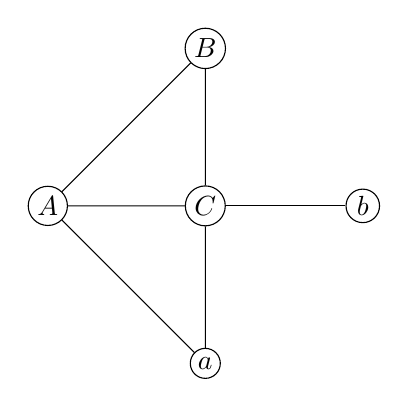
\begin{tikzpicture}[scale=1,every node/.style={draw,circle, inner sep=.05 cm}]
		% \foreach \i in {0,1}{
		% 	\node (\i1) at (\i-1,\i){$A_{\i}$};
		% 	% \node (\i0) at (\i,-1){$h_{\i}$};
		% 	}
		\node (01) at (-1,0){$A$};
		\node (11) at (1,2){$B$};
		\node (02) at (1,0){$C$};
		\node (0-1) at (1,-2){$a$};
		\node (03) at (3,0){$b$};
		\draw (02)--(01)--(11)--(02)--(0-1)--(01);
		\draw (02)--(03);
		% \draw (01)--(11)--(00)--(01);
		\end{tikzpicture}\]
% 	% https://q.uiver.app/#q=WzAsNixbMCwxLCJBIFxcYnVsbGV0Il0sWzEsMSwiQ1xcYnVsbGV0Il0sWzIsMSwiYlxcYnVsbGV0Il0sWzEsMiwiYVxcYnVsbGV0Il0sWzEsMCwiQlxcYnVsbGV0Il0sWzEsMywiRyJdLFswLDEsIiIsMCx7InN0eWxlIjp7ImhlYWQiOnsibmFtZSI6Im5vbmUifX19XSxbMSwyLCIiLDAseyJzdHlsZSI6eyJoZWFkIjp7Im5hbWUiOiJub25lIn19fV0sWzEsMywiIiwwLHsic3R5bGUiOnsiaGVhZCI6eyJuYW1lIjoibm9uZSJ9fX1dLFswLDMsIiIsMix7InN0eWxlIjp7ImhlYWQiOnsibmFtZSI6Im5vbmUifX19XSxbMSw0LCIiLDIseyJzdHlsZSI6eyJoZWFkIjp7Im5hbWUiOiJub25lIn19fV0sWzQsMCwiIiwyLHsic3R5bGUiOnsiaGVhZCI6eyJuYW1lIjoibm9uZSJ9fX1dXQ==
% \[\begin{tikzcd}
% 	& B\bullet \\
% 	{A \bullet} & C\bullet & b\bullet \\
% 	& a\bullet \\
% 	& G
% 	\arrow[no head, from=2-1, to=2-2]
% 	\arrow[no head, from=2-2, to=2-3]
% 	\arrow[no head, from=2-2, to=3-2]
% 	\arrow[no head, from=2-1, to=3-2]
% 	\arrow[no head, from=2-2, to=1-2]
% 	\arrow[no head, from=1-2, to=2-1]
% \end{tikzcd}\]
We label each vertex in $G$ by degree.
\[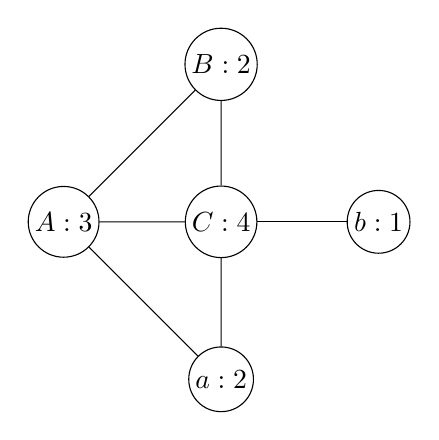
\begin{tikzpicture}[scale=1,every node/.style={draw,circle, inner sep=.05 cm}]
	% \foreach \i in {0,1}{
	% 	\node (\i1) at (\i-1,\i){$A_{\i}$};
	% 	% \node (\i0) at (\i,-1){$h_{\i}$};
	% 	}
	\node (01) at (-1,0){$A:3$};
	\node (11) at (1,2){$B:2$};
	\node (02) at (1,0){$C:4$};
	\node (0-1) at (1,-2){$a:2$};
	\node (03) at (3,0){$b:1$};
	\draw (02)--(01)--(11)--(02)--(0-1)--(01);
	\draw (02)--(03);
	% \draw (01)--(11)--(00)--(01);
	\end{tikzpicture}\]
Our partition of $V$ is $P = \{l_1,l_2,l_3,l_4\}$ where $l_1=\{b\}$, $l_2=\{a,B\}$, $l_3=\{A\}$, and $l_4=\{C\}$. As an example, note $N(A)=\{B,C,a\}$. Therefore, $A$ has two neighbors in $l_2$, namely, $a$ and $B$, and one neighbor in $l_4$, $C$. Thus, $cv(A)=(3,0,2,0,1)$. The reader is encouraged to construct the characterstic vectors for the remaining vertices. To check your work, the results are shown in the table below.
\begin{center}
% \begin{multicols}{2}
	\begin{tabular}{|c|c|c|c|c|c|}
		\hline
		vertices&A&B&C&a&b\\
		\hline
		cv&(3,0,2,0,1)&($2$,0,0,1,1)&($4$,1,2,1,0)&($2$,0,0,1,1)&($2$,0,0,0,1)\\
		\hline
	\end{tabular}\\
% \end{multicols}
\end{center}
\paragraph{}The last step of an iteration is to order the vectors lexicographically. We assign a new label to each vertex based on this ordering. Since 5 is the next integer after our initial 4 classes, first vertex in the order receives a new label of 5. Continue until every vertex has been relabelled. For example, vertex $b$ with characteristic vector $(2,0,0,0,1)$ receives a new label of 5. The result of applying this ordering and relabelling process to the vertices and characteristic vectors of this example is shown in the table and graph below.
\begin{center}
	% \begin{multicols}{2}
		\begin{tabular}{|c|c|c|c|c|c|}
			\hline
			vertices&A&B&C&a&b\\
			\hline
			cv&(3,0,2,0,1)&($2$,0,0,1,1)&($4$,1,2,1,0)&($2$,0,0,1,1)&($2$,0,0,0,1)\\
			\hline
			new label&7&6&8&6&5\\
			\hline
		\end{tabular}
	% \end{multicols}
	\end{center}
	\[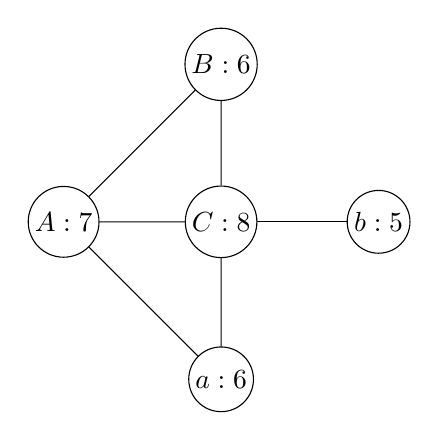
\begin{tikzpicture}[scale=1,every node/.style={draw,circle, inner sep=.05 cm}]
		% \foreach \i in {0,1}{
		% 	\node (\i1) at (\i-1,\i){$A_{\i}$};
		% 	% \node (\i0) at (\i,-1){$h_{\i}$};
		% 	}
		\node (01) at (-1,0){$A:7$};
		\node (11) at (1,2){$B:6$};
		\node (02) at (1,0){$C:8$};
		\node (0-1) at (1,-2){$a:6$};
		\node (03) at (3,0){$b:5$};
		\draw (02)--(01)--(11)--(02)--(0-1)--(01);
		\draw (02)--(03);
		% \draw (01)--(11)--(00)--(01);
		\end{tikzpicture}\]
	% Note that each vertex has a unique label. That is, there are no incomparable vertices, which means we have produced a canonical labeling of $V$.
\end{example}
	\paragraph{} We formalize the steps in the following algorithm.
	\begin{align*}
		&\textbf{WL}\\
	\textbf{Input:}&\;G=\{V,E\}\\
	\textbf{Initialize:}&\text{ Label vertices using degree}\\
	\textbf{Iterate:}&\text{ Produce characteristic vectors, order lexicographically and relabel}\\
	\textbf{Output:}&\text{ Graph }G \text{ with a canonical labelling of the vertex set }
	\end{align*}
	While it is likely clear that comparable vertices (those with different labels) in the output of WL are different, if two vertices $u$ and $v$ end up with the same label, it is not obvious that there exists an automorphism sending $u$ to $v$. However, this non-trivial result is shown in \cite{weisfeiler1968}. Hence, we can be sure that WL results in a canonical labelling for any simple graph.
	
	\begin{remark}
		In \cite{weisfeiler1968}, it is shown that WL will produce a canonical labelling for graphs with loops and/or multiple edges, not just simple graphs.
	\end{remark}The following example applies WL Canonical Labeling until a canonical labelling is produced.
	\begin{example}
        Given the graph $G$ below, we follow WL canonical labelling until the classes stabilize.\\
			\textbf{Input:}% https://q.uiver.app/?q=WzAsNSxbMCwwLCJcXGJ1bGxldCJdLFswLDEsIlxcYnVsbGV0Il0sWzEsMSwiXFxidWxsZXQiXSxbMiwxLCJcXGJ1bGxldCJdLFsxLDAsIlxcYnVsbGV0Il0sWzAsMSwiIiwwLHsic3R5bGUiOnsiaGVhZCI6eyJuYW1lIjoibm9uZSJ9fX1dLFsxLDIsIiIsMCx7InN0eWxlIjp7ImhlYWQiOnsibmFtZSI6Im5vbmUifX19XSxbMiwzLCIiLDAseyJzdHlsZSI6eyJoZWFkIjp7Im5hbWUiOiJub25lIn19fV0sWzEsNCwiIiwwLHsic3R5bGUiOnsiaGVhZCI6eyJuYW1lIjoibm9uZSJ9fX1dXQ==
    \[\begin{tikzcd}
	a\;\bullet & b\;\bullet \\
	c\;\bullet & d\;\bullet & e\;\bullet
	\arrow[no head, from=1-1, to=2-1]
	\arrow[no head, from=2-1, to=2-2]
	\arrow[no head, from=2-2, to=2-3]
	\arrow[no head, from=2-1, to=1-2]
\end{tikzcd}\]
Ordering the vertices of $G$ alphabetically, the adjaceny matrix of $G$ is as follows.
\[A(G)=\bordermatrix{
	&a&b&c&d&e\cr
	a&0&0&1&0&0\cr
	b&0&0&1&0&0\cr
	c&1&1&0&1&0\cr
	d&0&0&1&0&1\cr
	e&0&0&0&1&0
}\]
\textbf{I. Initialize:}
\begin{multicols}{2}
\begin{tabular}{|c|c|}
	\hline
	classes&label\\
	\hline
	\{c\}&3\\
	\{d\}&2\\
	\{a,b,e\}&1\\
	\hline
\end{tabular}\\
\[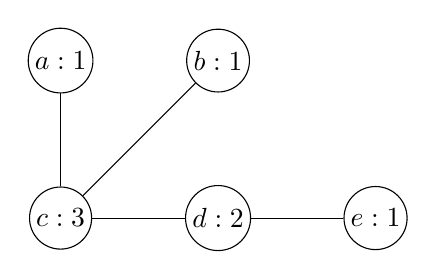
\begin{tikzpicture}[scale=1,every node/.style={draw,circle, inner sep=.05 cm}]
	% \foreach \i in {0,1}{
	% 	\node (\i1) at (\i-1,\i){$A_{\i}$};
	% 	% \node (\i0) at (\i,-1){$h_{\i}$};
	% 	}
	\node (01) at (-1,0){$c:3$};
	\node (11) at (-1,2){$a:1$};
	\node (02) at (1,2){$b:1$};
	\node (0-1) at (1,0){$d:2$};
	\node (03) at (3,0){$e:1$};
	\draw (11)--(01)--(0-1);
	\draw (01)--(02);
	\draw (0-1)--(03);
	% \draw (01)--(11)--(00)--(01);
	\end{tikzpicture}\]
% % https://q.uiver.app/?q=WzAsNSxbMCwwLCIxXFxidWxsZXQiXSxbMCwxLCIzXFxidWxsZXQiXSxbMSwxLCIyXFxidWxsZXQiXSxbMiwxLCIxXFxidWxsZXQiXSxbMSwwLCIxXFxidWxsZXQiXSxbMCwxLCIiLDAseyJzdHlsZSI6eyJoZWFkIjp7Im5hbWUiOiJub25lIn19fV0sWzEsMiwiIiwwLHsic3R5bGUiOnsiaGVhZCI6eyJuYW1lIjoibm9uZSJ9fX1dLFsyLDMsIiIsMCx7InN0eWxlIjp7ImhlYWQiOnsibmFtZSI6Im5vbmUifX19XSxbMSw0LCIiLDAseyJzdHlsZSI6eyJoZWFkIjp7Im5hbWUiOiJub25lIn19fV1d
% \[\begin{tikzcd}
% 	1\bullet & 1\bullet \\
% 	3\bullet & 2\bullet & 1\bullet
% 	\arrow[no head, from=1-1, to=2-1]
% 	\arrow[no head, from=2-1, to=2-2]
% 	\arrow[no head, from=2-2, to=2-3]
% 	\arrow[no head, from=2-1, to=1-2]
% \end{tikzcd}\]
\end{multicols}
\textbf{II. Generate Characteristic Vectors \& Relabel:}\\
\begin{multicols}{2}
\begin{tabular}{|c|c|c|}
	\hline
	classes&cv&relabel\\
	\hline
	\{c\}&(3,2,1,0)&7\\
	\{d\}&(2,1,0,1)&6\\
	\{e\}&(1,0,1,0)&5\\
	\{a,b\}&(1,0,0,1)&4\\
	\hline
\end{tabular}\\
\[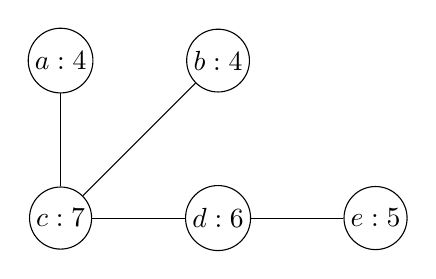
\begin{tikzpicture}[scale=1,every node/.style={draw,circle, inner sep=.05 cm}]
	% \foreach \i in {0,1}{
	% 	\node (\i1) at (\i-1,\i){$A_{\i}$};
	% 	% \node (\i0) at (\i,-1){$h_{\i}$};
	% 	}
	\node (01) at (-1,0){$c:7$};
	\node (11) at (-1,2){$a:4$};
	\node (02) at (1,2){$b:4$};
	\node (0-1) at (1,0){$d:6$};
	\node (03) at (3,0){$e:5$};
	\draw (11)--(01)--(0-1);
	\draw (01)--(02);
	\draw (0-1)--(03);
	% \draw (01)--(11)--(00)--(01);
	\end{tikzpicture}\]
% % https://q.uiver.app/?q=WzAsNSxbMCwwLCIoMSwwLDAsMSlcXGJ1bGxldCJdLFswLDEsIigzLDIsMSwwKVxcYnVsbGV0Il0sWzEsMSwiKDIsMSwwLDEpXFxidWxsZXQiXSxbMiwxLCIoMSwwLDEsMClcXGJ1bGxldCJdLFsxLDAsIigxLDAsMCwxKVxcYnVsbGV0Il0sWzAsMSwiIiwwLHsic3R5bGUiOnsiaGVhZCI6eyJuYW1lIjoibm9uZSJ9fX1dLFsxLDIsIiIsMCx7InN0eWxlIjp7ImhlYWQiOnsibmFtZSI6Im5vbmUifX19XSxbMiwzLCIiLDAseyJzdHlsZSI6eyJoZWFkIjp7Im5hbWUiOiJub25lIn19fV0sWzEsNCwiIiwwLHsic3R5bGUiOnsiaGVhZCI6eyJuYW1lIjoibm9uZSJ9fX1dXQ==
% \[\begin{tikzcd}
% 	{4\;\bullet} & {4\;\bullet} \\
% 	{7\;\bullet} & {6\;\bullet} & {5\;\bullet}
% 	\arrow[no head, from=1-1, to=2-1]
% 	\arrow[no head, from=2-1, to=2-2]
% 	\arrow[no head, from=2-2, to=2-3]
% 	\arrow[no head, from=2-1, to=1-2]
% \end{tikzcd}\]
\end{multicols}\newpage
\textbf{III. Iterate:} \\
Since the classes stay the same, the process terminates here. 
\begin{multicols}{2}
\begin{tabular}{|c|c|}
	\hline
	classes&cv\\
	\hline
	\{c\}&(7,2,0,1,0)\\
	\{d\}&(6,0,1,0,1)\\
	\{e\}&(5,0,0,1,0)\\
	\{a,b\}&(4,0,0,1,0)\\
	\hline
\end{tabular}\\
\[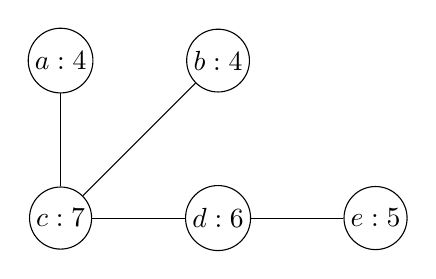
\begin{tikzpicture}[scale=1,every node/.style={draw,circle, inner sep=.05 cm}]
	% \foreach \i in {0,1}{
	% 	\node (\i1) at (\i-1,\i){$A_{\i}$};
	% 	% \node (\i0) at (\i,-1){$h_{\i}$};
	% 	}
	\node (01) at (-1,0){$c:7$};
	\node (11) at (-1,2){$a:4$};
	\node (02) at (1,2){$b:4$};
	\node (0-1) at (1,0){$d:6$};
	\node (03) at (3,0){$e:5$};
	\draw (11)--(01)--(0-1);
	\draw (01)--(02);
	\draw (0-1)--(03);
	% \draw (01)--(11)--(00)--(01);
	\end{tikzpicture}\]
% % https://q.uiver.app/?q=WzAsNSxbMCwwLCIoMSwwLDAsMSlcXGJ1bGxldCJdLFswLDEsIigzLDIsMSwwKVxcYnVsbGV0Il0sWzEsMSwiKDIsMSwwLDEpXFxidWxsZXQiXSxbMiwxLCIoMSwwLDEsMClcXGJ1bGxldCJdLFsxLDAsIigxLDAsMCwxKVxcYnVsbGV0Il0sWzAsMSwiIiwwLHsic3R5bGUiOnsiaGVhZCI6eyJuYW1lIjoibm9uZSJ9fX1dLFsxLDIsIiIsMCx7InN0eWxlIjp7ImhlYWQiOnsibmFtZSI6Im5vbmUifX19XSxbMiwzLCIiLDAseyJzdHlsZSI6eyJoZWFkIjp7Im5hbWUiOiJub25lIn19fV0sWzEsNCwiIiwwLHsic3R5bGUiOnsiaGVhZCI6eyJuYW1lIjoibm9uZSJ9fX1dXQ==
% \[\begin{tikzcd}
% 	{4\;\bullet} & {4\;\bullet} \\
% 	{7\;\bullet} & {6\;\bullet} & {5\;\bullet}
% 	\arrow[no head, from=1-1, to=2-1]
% 	\arrow[no head, from=2-1, to=2-2]
% 	\arrow[no head, from=2-2, to=2-3]
% 	\arrow[no head, from=2-1, to=1-2]
% \end{tikzcd}\]
\end{multicols}
The following is a canonical form of $G$ generated by WL.
\[Canon(G)=\bordermatrix{
	&a&b&e&d&c\cr
	a&0&0&0&0&1\cr
	b&0&0&0&0&1\cr
	e&0&0&0&1&0\cr
	d&0&0&1&0&1\cr
	c&1&1&0&1&0
}\]
% \[Canon(G)=\begin{pmatrix}
% 	0&0&0&0&1\\
% 	0&0&0&0&1\\
% 	0&0&0&1&0\\
% 	0&0&1&0&1\\
% 	1&1&0&1&0
% \end{pmatrix}\]
% Using $Canon(G)$, we generate a graph labelled using the first entry of each characteristic vector. 
% % https://q.uiver.app/?q=WzAsNSxbMCwwLCIxXFxidWxsZXQiXSxbMCwxLCI0XFxidWxsZXQiXSxbMSwxLCIzXFxidWxsZXQiXSxbMiwxLCIyXFxidWxsZXQiXSxbMSwwLCIxXFxidWxsZXQiXSxbMCwxLCIiLDAseyJzdHlsZSI6eyJoZWFkIjp7Im5hbWUiOiJub25lIn19fV0sWzEsMiwiIiwwLHsic3R5bGUiOnsiaGVhZCI6eyJuYW1lIjoibm9uZSJ9fX1dLFsyLDMsIiIsMCx7InN0eWxlIjp7ImhlYWQiOnsibmFtZSI6Im5vbmUifX19XSxbMSw0LCIiLDAseyJzdHlsZSI6eyJoZWFkIjp7Im5hbWUiOiJub25lIn19fV1d
% \[\begin{tikzcd}
% 	4\bullet & 4\bullet \\
% 	7\bullet & 6\bullet & 5\bullet
% 	\arrow[no head, from=1-1, to=2-1]
% 	\arrow[no head, from=2-1, to=2-2]
% 	\arrow[no head, from=2-2, to=2-3]
% 	\arrow[no head, from=2-1, to=1-2]
% \end{tikzcd}\]

	





   
Notice that $a$ and $b$ are in the same class, that is, $a$ and $b$ are incomparable. Since the relevant result from \cite{weisfeiler1968} mentioned above, ensures that this is a canonical form of $G$. Hence, there exist a graph automorphism sending $a$ to $b$. The function, $f:\{a,b,c,d,e\}\rightarrow\{a,b,c,d,e\}$, defined by \[f(u)=\begin{cases}
	b,\;u=a\\
	a,\;u=b\\
	u,\;u\ne a,b
\end{cases}\]is such a function.
% If two vertices $u,v\in V$ are in the same class when the algorithm terminates, then there exists an automorphism sending $u$ to $v$ \cite{weisfeiler1968}. Thus, the partial ordering of $V$ given by such classes is a canonical form by Definition 2.7.
% On the other hand, if each vertex has a unique class when the algorithm terminates, then the partial ordering of $V$ given by the classes leaves no incomparable vertices. In this case, the ordering on $V$ given by the classes is a canonical form as well, satisfying Definition 2.7 trivially. 
    \end{example} 

	\begin{remark}
		Since WL iteratively produces partitions of vertex sets, it is also called \textit{color refinement}. The color of a vertex is its class at any given iteration. 
	\end{remark}
\subsection{A Non-Isomorphism Test}
As mentioned in the previous subsection, we can use a canonization algorithm to produce a graph identification algorithm. However, unless we add extra machinery, canonization is not sufficient for graph identification. In that case, we can only hope to produce an algorithm that can determine two graphs are not isomorphic. In what follows, we present such an algorithm based on WL, the \textit{WL Non-Isomorphism Test}, adopted from \cite{shervashidze2011weisfeiler}. This test differs from WL in two key ways. First, the input of WL Non-Isomorphism Test is two graphs rather than a single graph.  WL is applied to each graph at the same time, where new vertex labels for both graphs come from same alphabet. Second, at initialization, a label string is generated for each graph $G$, denoted $s(G)$, using the initial labels as follows. The $k^{th}$ entry in a label string for a graph $G$ is the number of vertices of $G$ with label $k$. After each iteration, a new label string is generated based on the new labels, then concatenated to the end of the old string. If the graphs have different strings at any step then the algorithm terminates immediately, returning that the two graphs are not isomorphic. 
		\paragraph{}\begin{align*}
			&\textbf{WL Non-Isomorphism Test }\\
		\textbf{Input:}&\text{ Graphs }G=\{V,E\},\;G'=\{V',E'\}\\
		\textbf{Initialize:}&\text{ Label the vertices using degree}\\
		&\text{Generate and compare label strings}\\
		&\text{If strings are not equal, terminate}\\
		\textbf{Iterate:}&\text{ Produce characteristic vectors for all vertices in }G\text{ and }G'\\
		&\text{ Order characteristic vectors, relabel}\\
		&\text{If classes did not change, terminate}\\
		&\text{Generate new label string }\\
		&\text{If strings are not equal, terminate}\\
		\textbf{Output:}&\text{ A graph isomorphism from $G$ to $G'$ does not exist }\\&\text{or NULL}
		\end{align*}
		\begin{example}
			This example applies the WL Non-Isomorphism Test to $H$ and $H'$.
			\begin{multicols}{2}
				$H$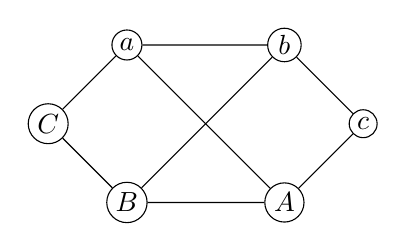
\begin{tikzpicture}[scale=1,every node/.style={draw,circle, inner sep=.05 cm}]
				% \foreach \i in {0,1}{
				% 	\node (\i1) at (\i-1,\i){$A_{\i}$};
				% 	% \node (\i0) at (\i,-1){$h_{\i}$};
				% 	}
				\node (-10) at (-1,0){$C$};
				\node (02) at (0,1){$a$};
				\node (0-2) at (0,-1){$B$};
				\node (32) at (2,1){$b$};
				\node (3-2) at (2,-1){$A$};
				\node (50) at (3,0){$c$};
				\draw (02)--(-10)--(0-2);
				\draw (3-2)--(02)--(32);
				\draw (32)--(0-2)--(3-2);
				\draw (32)--(50)--(3-2);
				% \draw (01)--(11)--(00)--(01);
				\end{tikzpicture}\\
				$H'$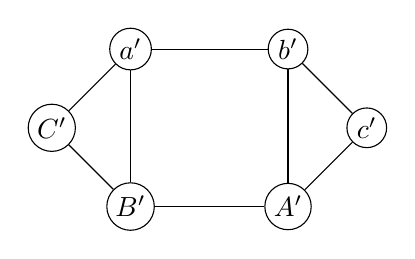
\begin{tikzpicture}[scale=1,every node/.style={draw,circle, inner sep=.05 cm}]
					% \foreach \i in {0,1}{
					% 	\node (\i1) at (\i-1,\i){$A_{\i}$};
					% 	% \node (\i0) at (\i,-1){$h_{\i}$};
					% 	}
					\node (-10) at (-1,0){$C'$};
					\node (02) at (0,1){$a'$};
					\node (0-2) at (0,-1){$B'$};
					\node (32) at (2,1){$b'$};
					\node (3-2) at (2,-1){$A'$};
					\node (50) at (3,0){$c'$};
					\draw (02)--(-10)--(0-2);
					\draw (3-2)--(0-2)--(02)--(32)--(3-2);
					% \draw (0-2)--(3-2);
					\draw (32)--(50)--(3-2);
					% \draw (01)--(11)--(00)--(01);
					\end{tikzpicture}
			\end{multicols}
% 			   % https://q.uiver.app/?q=WzAsMTQsWzIsMCwiXFxidWxsZXQiXSxbMywxLCJcXGJ1bGxldCJdLFsyLDIsIlxcYnVsbGV0Il0sWzEsMiwiXFxidWxsZXQiXSxbMCwxLCJcXGJ1bGxldCJdLFsxLDAsIlxcYnVsbGV0Il0sWzcsMCwiXFxidWxsZXQiXSxbOCwxLCJcXGJ1bGxldCJdLFs3LDIsIlxcYnVsbGV0Il0sWzYsMiwiXFxidWxsZXQiXSxbNSwxLCJcXGJ1bGxldCJdLFs2LDAsIlxcYnVsbGV0Il0sWzEsMywiSCJdLFs3LDMsIkgnIl0sWzAsMSwiIiwwLHsic3R5bGUiOnsiaGVhZCI6eyJuYW1lIjoibm9uZSJ9fX1dLFsxLDIsIiIsMCx7InN0eWxlIjp7ImhlYWQiOnsibmFtZSI6Im5vbmUifX19XSxbMiwzLCIiLDAseyJzdHlsZSI6eyJoZWFkIjp7Im5hbWUiOiJub25lIn19fV0sWzMsNCwiIiwwLHsic3R5bGUiOnsiaGVhZCI6eyJuYW1lIjoibm9uZSJ9fX1dLFs0LDUsIiIsMCx7InN0eWxlIjp7ImhlYWQiOnsibmFtZSI6Im5vbmUifX19XSxbNiw3LCIiLDAseyJzdHlsZSI6eyJoZWFkIjp7Im5hbWUiOiJub25lIn19fV0sWzcsOCwiIiwwLHsic3R5bGUiOnsiaGVhZCI6eyJuYW1lIjoibm9uZSJ9fX1dLFs4LDksIiIsMCx7InN0eWxlIjp7ImhlYWQiOnsibmFtZSI6Im5vbmUifX19XSxbOSwxMCwiIiwwLHsic3R5bGUiOnsiaGVhZCI6eyJuYW1lIjoibm9uZSJ9fX1dLFsxMCwxMSwiIiwwLHsic3R5bGUiOnsiaGVhZCI6eyJuYW1lIjoibm9uZSJ9fX1dLFsxMSw2LCIiLDAseyJzdHlsZSI6eyJoZWFkIjp7Im5hbWUiOiJub25lIn19fV0sWzExLDksIiIsMSx7InN0eWxlIjp7ImhlYWQiOnsibmFtZSI6Im5vbmUifX19XSxbNiw4LCIiLDEseyJzdHlsZSI6eyJoZWFkIjp7Im5hbWUiOiJub25lIn19fV0sWzUsMCwiIiwxLHsic3R5bGUiOnsiaGVhZCI6eyJuYW1lIjoibm9uZSJ9fX1dLFszLDAsIiIsMSx7InN0eWxlIjp7ImhlYWQiOnsibmFtZSI6Im5vbmUifX19XSxbNSwyLCIiLDEseyJzdHlsZSI6eyJoZWFkIjp7Im5hbWUiOiJub25lIn19fV1d
% \[\begin{tikzcd}[ampersand replacement=\&]
% 	\& a\;\bullet \& b\;\bullet \&\&\&\& a'\;\bullet \& b'\;\bullet \\
% 	C\;\bullet \&\&\& c\;\bullet \&\& C'\;\bullet \&\&\& c'\;\bullet \\
% 	\& B\;\;\bullet \& A\;\bullet \&\&\&\& B'\;\bullet \& A'\;\bullet \\
% 	\& H \&\&\&\&\&\& {H'}
% 	\arrow[no head, from=1-3, to=2-4]
% 	\arrow[no head, from=2-4, to=3-3]
% 	\arrow[no head, from=3-3, to=3-2]
% 	\arrow[no head, from=3-2, to=2-1]
% 	\arrow[no head, from=2-1, to=1-2]
% 	\arrow[no head, from=1-8, to=2-9]
% 	\arrow[no head, from=2-9, to=3-8]
% 	\arrow[no head, from=3-8, to=3-7]
% 	\arrow[no head, from=3-7, to=2-6]
% 	\arrow[no head, from=2-6, to=1-7]
% 	\arrow[no head, from=1-7, to=1-8]
% 	\arrow[no head, from=1-7, to=3-7]
% 	\arrow[no head, from=1-8, to=3-8]
% 	\arrow[no head, from=1-2, to=1-3]
% 	\arrow[no head, from=3-2, to=1-3]
% 	\arrow[no head, from=1-2, to=3-3]
% \end{tikzcd}\]
\newpage
\textbf{I. Initialize:} Label the vertices by their degree and construct label strings.
\begin{multicols}{2}
	$H$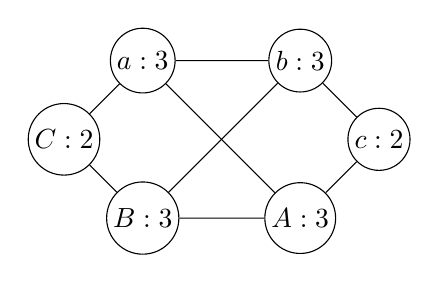
\begin{tikzpicture}[scale=1,every node/.style={draw,circle, inner sep=.05 cm}]
	% \foreach \i in {0,1}{
	% 	\node (\i1) at (\i-1,\i){$A_{\i}$};
	% 	% \node (\i0) at (\i,-1){$h_{\i}$};
	% 	}
	\node (-10) at (-1,0){$C:2$};
	\node (02) at (0,1){$a:3$};
	\node (0-2) at (0,-1){$B:3$};
	\node (32) at (2,1){$b:3$};
	\node (3-2) at (2,-1){$A:3$};
	\node (50) at (3,0){$c:2$};
	\draw (02)--(-10)--(0-2);
	\draw (3-2)--(02)--(32);
	\draw (32)--(0-2)--(3-2);
	\draw (32)--(50)--(3-2);
	% \draw (01)--(11)--(00)--(01);
	\end{tikzpicture}\\
	$H'$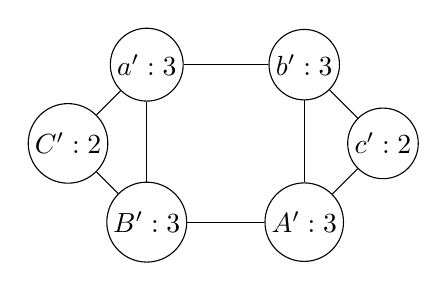
\begin{tikzpicture}[scale=1,every node/.style={draw,circle, inner sep=.05 cm}]
		% \foreach \i in {0,1}{
		% 	\node (\i1) at (\i-1,\i){$A_{\i}$};
		% 	% \node (\i0) at (\i,-1){$h_{\i}$};
		% 	}
		\node (-10) at (-1,0){$C':2$};
		\node (02) at (0,1){$a':3$};
		\node (0-2) at (0,-1){$B':3$};
		\node (32) at (2,1){$b':3$};
		\node (3-2) at (2,-1){$A':3$};
		\node (50) at (3,0){$c':2$};
		\draw (02)--(-10)--(0-2);
		\draw (3-2)--(0-2)--(02)--(32)--(3-2);
		% \draw (0-2)--(3-2);
		\draw (32)--(50)--(3-2);
		% \draw (01)--(11)--(00)--(01);
		\end{tikzpicture}
\end{multicols}
% % https://q.uiver.app/?q=WzAsMTIsWzIsMCwiMyJdLFszLDEsIjIiXSxbMiwyLCIzIl0sWzEsMiwiMyJdLFswLDEsIjIiXSxbMSwwLCIzIl0sWzcsMCwiMyJdLFs4LDEsIjIiXSxbNywyLCIzIl0sWzYsMiwiMyJdLFs1LDEsIjIiXSxbNiwwLCIzIl0sWzAsMSwiIiwwLHsic3R5bGUiOnsiaGVhZCI6eyJuYW1lIjoibm9uZSJ9fX1dLFsxLDIsIiIsMCx7InN0eWxlIjp7ImhlYWQiOnsibmFtZSI6Im5vbmUifX19XSxbMiwzLCIiLDAseyJzdHlsZSI6eyJoZWFkIjp7Im5hbWUiOiJub25lIn19fV0sWzMsNCwiIiwwLHsic3R5bGUiOnsiaGVhZCI6eyJuYW1lIjoibm9uZSJ9fX1dLFs0LDUsIiIsMCx7InN0eWxlIjp7ImhlYWQiOnsibmFtZSI6Im5vbmUifX19XSxbNiw3LCIiLDAseyJzdHlsZSI6eyJoZWFkIjp7Im5hbWUiOiJub25lIn19fV0sWzcsOCwiIiwwLHsic3R5bGUiOnsiaGVhZCI6eyJuYW1lIjoibm9uZSJ9fX1dLFs4LDksIiIsMCx7InN0eWxlIjp7ImhlYWQiOnsibmFtZSI6Im5vbmUifX19XSxbOSwxMCwiIiwwLHsic3R5bGUiOnsiaGVhZCI6eyJuYW1lIjoibm9uZSJ9fX1dLFsxMCwxMSwiIiwwLHsic3R5bGUiOnsiaGVhZCI6eyJuYW1lIjoibm9uZSJ9fX1dLFsxMSw2LCIiLDAseyJzdHlsZSI6eyJoZWFkIjp7Im5hbWUiOiJub25lIn19fV0sWzExLDksIiIsMSx7InN0eWxlIjp7ImhlYWQiOnsibmFtZSI6Im5vbmUifX19XSxbNiw4LCIiLDEseyJzdHlsZSI6eyJoZWFkIjp7Im5hbWUiOiJub25lIn19fV0sWzUsMCwiIiwxLHsic3R5bGUiOnsiaGVhZCI6eyJuYW1lIjoibm9uZSJ9fX1dLFszLDAsIiIsMSx7InN0eWxlIjp7ImhlYWQiOnsibmFtZSI6Im5vbmUifX19XSxbNSwyLCIiLDEseyJzdHlsZSI6eyJoZWFkIjp7Im5hbWUiOiJub25lIn19fV1d
% \[\begin{tikzcd}[ampersand replacement=\&]
% 	\& 3 \& 3 \&\&\&\& 3 \& 3 \\
% 	2 \&\&\& 2 \&\& 2 \&\&\& 2 \\
% 	\& 3 \& 3 \&\&\&\& 3 \& 3
% 	\arrow[no head, from=1-3, to=2-4]
% 	\arrow[no head, from=2-4, to=3-3]
% 	\arrow[no head, from=3-3, to=3-2]
% 	\arrow[no head, from=3-2, to=2-1]
% 	\arrow[no head, from=2-1, to=1-2]
% 	\arrow[no head, from=1-8, to=2-9]
% 	\arrow[no head, from=2-9, to=3-8]
% 	\arrow[no head, from=3-8, to=3-7]
% 	\arrow[no head, from=3-7, to=2-6]
% 	\arrow[no head, from=2-6, to=1-7]
% 	\arrow[no head, from=1-7, to=1-8]
% 	\arrow[no head, from=1-7, to=3-7]
% 	\arrow[no head, from=1-8, to=3-8]
% 	\arrow[no head, from=1-2, to=1-3]
% 	\arrow[no head, from=3-2, to=1-3]
% 	\arrow[no head, from=1-2, to=3-3]
% \end{tikzcd}\]
\begin{multicols}{2}
\begin{tabular}{|c|c|}
	\hline
	classes&label\\
	\hline
	\{a,b,A,B\}&3\\
	\{c,C\}&2\\
	\{\}&1\\
	\hline
\end{tabular}
$s(H) = (024)$ \\

\begin{tabular}{|c|c|}
	\hline
	classes&label\\
	\hline
	\{a',b',A',B'\}&3\\
	\{c',C'\}&2\\
	\{\}&1\\
	\hline
\end{tabular}
$s(H') = (024)$
\end{multicols}
\textbf{II. Generate Characteristic Vectors \& Relabel:}\\
Notice that the labels do not change from the previous step, so the process terminates after relabelling.
\begin{multicols}{2}
\begin{tabular}{|c|c|c|}
	\hline
	classes&cv&label\\
	\hline
	\{a,b,A,B\}&(3,0,1,2)&5\\
	\{c,C\}&(2,0,0,2)&4\\
	\{\}&&\\
	\hline
\end{tabular}

\begin{tabular}{|c|c|c|}
	\hline
	classes&cv&label\\
	\hline
	\{a',b',A',B'\}&(3,0,1,2)&5\\
	\{c',C'\}&(2,0,0,2)&4\\
	\{\}&&\\
	\hline
\end{tabular}
\end{multicols}

% Next, produce characteristic vectors.
% % https://q.uiver.app/?q=WzAsMTIsWzIsMCwiKDMsMCwxLDIpIl0sWzMsMSwiKDIsMCwwLDIpIl0sWzIsMiwiKDMsMCwxLDIpIl0sWzEsMiwiKDMsMCwxLDIpIl0sWzAsMSwiKDIsMCwwLDIpIl0sWzEsMCwiKDMsMCwxLDIpIl0sWzIsMywiKDMsMCwxLDIpIl0sWzMsNCwiKDIsMCwwLDIpIl0sWzIsNSwiKDMsMCwxLDIpIl0sWzEsNSwiKDMsMCwxLDIpIl0sWzAsNCwiKDIsMCwwLDIpIl0sWzEsMywiKDMsMCwxLDIpIl0sWzAsMSwiIiwwLHsic3R5bGUiOnsiaGVhZCI6eyJuYW1lIjoibm9uZSJ9fX1dLFsxLDIsIiIsMCx7InN0eWxlIjp7ImhlYWQiOnsibmFtZSI6Im5vbmUifX19XSxbMiwzLCIiLDAseyJzdHlsZSI6eyJoZWFkIjp7Im5hbWUiOiJub25lIn19fV0sWzMsNCwiIiwwLHsic3R5bGUiOnsiaGVhZCI6eyJuYW1lIjoibm9uZSJ9fX1dLFs0LDUsIiIsMCx7InN0eWxlIjp7ImhlYWQiOnsibmFtZSI6Im5vbmUifX19XSxbNiw3LCIiLDAseyJzdHlsZSI6eyJoZWFkIjp7Im5hbWUiOiJub25lIn19fV0sWzcsOCwiIiwwLHsic3R5bGUiOnsiaGVhZCI6eyJuYW1lIjoibm9uZSJ9fX1dLFs4LDksIiIsMCx7InN0eWxlIjp7ImhlYWQiOnsibmFtZSI6Im5vbmUifX19XSxbOSwxMCwiIiwwLHsic3R5bGUiOnsiaGVhZCI6eyJuYW1lIjoibm9uZSJ9fX1dLFsxMCwxMSwiIiwwLHsic3R5bGUiOnsiaGVhZCI6eyJuYW1lIjoibm9uZSJ9fX1dLFsxMSw2LCIiLDAseyJzdHlsZSI6eyJoZWFkIjp7Im5hbWUiOiJub25lIn19fV0sWzExLDksIiIsMSx7InN0eWxlIjp7ImhlYWQiOnsibmFtZSI6Im5vbmUifX19XSxbNiw4LCIiLDEseyJzdHlsZSI6eyJoZWFkIjp7Im5hbWUiOiJub25lIn19fV0sWzUsMCwiIiwxLHsic3R5bGUiOnsiaGVhZCI6eyJuYW1lIjoibm9uZSJ9fX1dLFszLDAsIiIsMSx7InN0eWxlIjp7ImhlYWQiOnsibmFtZSI6Im5vbmUifX19XSxbNSwyLCIiLDEseyJzdHlsZSI6eyJoZWFkIjp7Im5hbWUiOiJub25lIn19fV1d
% \[\begin{tikzcd}[ampersand replacement=\&]
% 	\& {(3,0,1,2)} \& {(3,0,1,2)} \\
% 	{(2,0,0,2)} \&\&\& {(2,0,0,2)} \\
% 	\& {(3,0,1,2)} \& {(3,0,1,2)} \\
% 	\& {(3,0,1,2)} \& {(3,0,1,2)} \\
% 	{(2,0,0,2)} \&\&\& {(2,0,0,2)} \\
% 	\& {(3,0,1,2)} \& {(3,0,1,2)}
% 	\arrow[no head, from=1-3, to=2-4]
% 	\arrow[no head, from=2-4, to=3-3]
% 	\arrow[no head, from=3-3, to=3-2]
% 	\arrow[no head, from=3-2, to=2-1]
% 	\arrow[no head, from=2-1, to=1-2]
% 	\arrow[no head, from=4-3, to=5-4]
% 	\arrow[no head, from=5-4, to=6-3]
% 	\arrow[no head, from=6-3, to=6-2]
% 	\arrow[no head, from=6-2, to=5-1]
% 	\arrow[no head, from=5-1, to=4-2]
% 	\arrow[no head, from=4-2, to=4-3]
% 	\arrow[no head, from=4-2, to=6-2]
% 	\arrow[no head, from=4-3, to=6-3]
% 	\arrow[no head, from=1-2, to=1-3]
% 	\arrow[no head, from=3-2, to=1-3]
% 	\arrow[no head, from=1-2, to=3-3]
% \end{tikzcd}\]
% Order the vectors and relabel.
% % https://q.uiver.app/?q=WzAsMTIsWzIsMCwiMiJdLFszLDEsIjEiXSxbMiwyLCIyIl0sWzEsMiwiMiJdLFswLDEsIjEiXSxbMSwwLCIyIl0sWzIsMywiMiJdLFszLDQsIjEiXSxbMiw1LCIyIl0sWzEsNSwiMiJdLFswLDQsIjEiXSxbMSwzLCIyIl0sWzAsMSwiIiwwLHsic3R5bGUiOnsiaGVhZCI6eyJuYW1lIjoibm9uZSJ9fX1dLFsxLDIsIiIsMCx7InN0eWxlIjp7ImhlYWQiOnsibmFtZSI6Im5vbmUifX19XSxbMiwzLCIiLDAseyJzdHlsZSI6eyJoZWFkIjp7Im5hbWUiOiJub25lIn19fV0sWzMsNCwiIiwwLHsic3R5bGUiOnsiaGVhZCI6eyJuYW1lIjoibm9uZSJ9fX1dLFs0LDUsIiIsMCx7InN0eWxlIjp7ImhlYWQiOnsibmFtZSI6Im5vbmUifX19XSxbNiw3LCIiLDAseyJzdHlsZSI6eyJoZWFkIjp7Im5hbWUiOiJub25lIn19fV0sWzcsOCwiIiwwLHsic3R5bGUiOnsiaGVhZCI6eyJuYW1lIjoibm9uZSJ9fX1dLFs4LDksIiIsMCx7InN0eWxlIjp7ImhlYWQiOnsibmFtZSI6Im5vbmUifX19XSxbOSwxMCwiIiwwLHsic3R5bGUiOnsiaGVhZCI6eyJuYW1lIjoibm9uZSJ9fX1dLFsxMCwxMSwiIiwwLHsic3R5bGUiOnsiaGVhZCI6eyJuYW1lIjoibm9uZSJ9fX1dLFsxMSw2LCIiLDAseyJzdHlsZSI6eyJoZWFkIjp7Im5hbWUiOiJub25lIn19fV0sWzExLDksIiIsMSx7InN0eWxlIjp7ImhlYWQiOnsibmFtZSI6Im5vbmUifX19XSxbNiw4LCIiLDEseyJzdHlsZSI6eyJoZWFkIjp7Im5hbWUiOiJub25lIn19fV0sWzUsMCwiIiwxLHsic3R5bGUiOnsiaGVhZCI6eyJuYW1lIjoibm9uZSJ9fX1dLFszLDAsIiIsMSx7InN0eWxlIjp7ImhlYWQiOnsibmFtZSI6Im5vbmUifX19XSxbNSwyLCIiLDEseyJzdHlsZSI6eyJoZWFkIjp7Im5hbWUiOiJub25lIn19fV1d
% \[\begin{tikzcd}[ampersand replacement=\&]
% 	\& 2 \& 2 \\
% 	1 \&\&\& 1 \\
% 	\& 2 \& 2 \\
% 	\& 2 \& 2 \\
% 	1 \&\&\& 1 \\
% 	\& 2 \& 2
% 	\arrow[no head, from=1-3, to=2-4]
% 	\arrow[no head, from=2-4, to=3-3]
% 	\arrow[no head, from=3-3, to=3-2]
% 	\arrow[no head, from=3-2, to=2-1]
% 	\arrow[no head, from=2-1, to=1-2]
% 	\arrow[no head, from=4-3, to=5-4]
% 	\arrow[no head, from=5-4, to=6-3]
% 	\arrow[no head, from=6-3, to=6-2]
% 	\arrow[no head, from=6-2, to=5-1]
% 	\arrow[no head, from=5-1, to=4-2]
% 	\arrow[no head, from=4-2, to=4-3]
% 	\arrow[no head, from=4-2, to=6-2]
% 	\arrow[no head, from=4-3, to=6-3]
% 	\arrow[no head, from=1-2, to=1-3]
% 	\arrow[no head, from=3-2, to=1-3]
% 	\arrow[no head, from=1-2, to=3-3]
% \end{tikzcd}\]
% Iterate.
% % https://q.uiver.app/?q=WzAsMTIsWzIsMCwiKDIsMSwyKSJdLFszLDEsIigxLDAsMikiXSxbMiwyLCIoMiwxLDIpIl0sWzEsMiwiKDIsMSwyKSJdLFswLDEsIigxLDAsMikiXSxbMSwwLCIoMiwxLDIpIl0sWzIsMywiKDIsMSwyKSJdLFszLDQsIigxLDAsMikiXSxbMiw1LCIoMiwxLDIpIl0sWzAsNCwiKDEsMCwyKSJdLFsxLDMsIigyLDEsMikiXSxbMSw1LCIoMiwxLDIpIl0sWzAsMSwiIiwwLHsic3R5bGUiOnsiaGVhZCI6eyJuYW1lIjoibm9uZSJ9fX1dLFsxLDIsIiIsMCx7InN0eWxlIjp7ImhlYWQiOnsibmFtZSI6Im5vbmUifX19XSxbMiwzLCIiLDAseyJzdHlsZSI6eyJoZWFkIjp7Im5hbWUiOiJub25lIn19fV0sWzMsNCwiIiwwLHsic3R5bGUiOnsiaGVhZCI6eyJuYW1lIjoibm9uZSJ9fX1dLFs0LDUsIiIsMCx7InN0eWxlIjp7ImhlYWQiOnsibmFtZSI6Im5vbmUifX19XSxbNiw3LCIiLDAseyJzdHlsZSI6eyJoZWFkIjp7Im5hbWUiOiJub25lIn19fV0sWzcsOCwiIiwwLHsic3R5bGUiOnsiaGVhZCI6eyJuYW1lIjoibm9uZSJ9fX1dLFs5LDEwLCIiLDAseyJzdHlsZSI6eyJoZWFkIjp7Im5hbWUiOiJub25lIn19fV0sWzEwLDYsIiIsMCx7InN0eWxlIjp7ImhlYWQiOnsibmFtZSI6Im5vbmUifX19XSxbNiw4LCIiLDEseyJzdHlsZSI6eyJoZWFkIjp7Im5hbWUiOiJub25lIn19fV0sWzUsMCwiIiwxLHsic3R5bGUiOnsiaGVhZCI6eyJuYW1lIjoibm9uZSJ9fX1dLFszLDAsIiIsMSx7InN0eWxlIjp7ImhlYWQiOnsibmFtZSI6Im5vbmUifX19XSxbNSwyLCIiLDEseyJzdHlsZSI6eyJoZWFkIjp7Im5hbWUiOiJub25lIn19fV0sWzgsMTEsIiIsMCx7InN0eWxlIjp7ImhlYWQiOnsibmFtZSI6Im5vbmUifX19XSxbMTEsOSwiIiwwLHsic3R5bGUiOnsiaGVhZCI6eyJuYW1lIjoibm9uZSJ9fX1dLFsxMCwxMSwiIiwxLHsic3R5bGUiOnsiaGVhZCI6eyJuYW1lIjoibm9uZSJ9fX1dXQ==
% \[\begin{tikzcd}[ampersand replacement=\&]
% 	\& {(2,1,2)} \& {(2,1,2)} \\
% 	{(1,0,2)} \&\&\& {(1,0,2)} \\
% 	\& {(2,1,2)} \& {(2,1,2)} \\
% 	\& {(2,1,2)} \& {(2,1,2)} \\
% 	{(1,0,2)} \&\&\& {(1,0,2)} \\
% 	\& {(2,1,2)} \& {(2,1,2)}
% 	\arrow[no head, from=1-3, to=2-4]
% 	\arrow[no head, from=2-4, to=3-3]
% 	\arrow[no head, from=3-3, to=3-2]
% 	\arrow[no head, from=3-2, to=2-1]
% 	\arrow[no head, from=2-1, to=1-2]
% 	\arrow[no head, from=4-3, to=5-4]
% 	\arrow[no head, from=5-4, to=6-3]
% 	\arrow[no head, from=5-1, to=4-2]
% 	\arrow[no head, from=4-2, to=4-3]
% 	\arrow[no head, from=4-3, to=6-3]
% 	\arrow[no head, from=1-2, to=1-3]
% 	\arrow[no head, from=3-2, to=1-3]
% 	\arrow[no head, from=1-2, to=3-3]
% 	\arrow[no head, from=6-3, to=6-2]
% 	\arrow[no head, from=6-2, to=5-1]
% 	\arrow[no head, from=4-2, to=6-2]
% \end{tikzcd}\]
% % https://q.uiver.app/?q=WzAsMTIsWzIsMCwiMiJdLFszLDEsIjEiXSxbMiwyLCIyIl0sWzEsMiwiMiJdLFswLDEsIjEiXSxbMSwwLCIyIl0sWzIsMywiMiJdLFszLDQsIjEiXSxbMiw1LCIyIl0sWzEsNSwiMiJdLFswLDQsIjEiXSxbMSwzLCIyIl0sWzAsMSwiIiwwLHsic3R5bGUiOnsiaGVhZCI6eyJuYW1lIjoibm9uZSJ9fX1dLFsxLDIsIiIsMCx7InN0eWxlIjp7ImhlYWQiOnsibmFtZSI6Im5vbmUifX19XSxbMiwzLCIiLDAseyJzdHlsZSI6eyJoZWFkIjp7Im5hbWUiOiJub25lIn19fV0sWzMsNCwiIiwwLHsic3R5bGUiOnsiaGVhZCI6eyJuYW1lIjoibm9uZSJ9fX1dLFs0LDUsIiIsMCx7InN0eWxlIjp7ImhlYWQiOnsibmFtZSI6Im5vbmUifX19XSxbNiw3LCIiLDAseyJzdHlsZSI6eyJoZWFkIjp7Im5hbWUiOiJub25lIn19fV0sWzcsOCwiIiwwLHsic3R5bGUiOnsiaGVhZCI6eyJuYW1lIjoibm9uZSJ9fX1dLFs4LDksIiIsMCx7InN0eWxlIjp7ImhlYWQiOnsibmFtZSI6Im5vbmUifX19XSxbOSwxMCwiIiwwLHsic3R5bGUiOnsiaGVhZCI6eyJuYW1lIjoibm9uZSJ9fX1dLFsxMCwxMSwiIiwwLHsic3R5bGUiOnsiaGVhZCI6eyJuYW1lIjoibm9uZSJ9fX1dLFsxMSw2LCIiLDAseyJzdHlsZSI6eyJoZWFkIjp7Im5hbWUiOiJub25lIn19fV0sWzExLDksIiIsMSx7InN0eWxlIjp7ImhlYWQiOnsibmFtZSI6Im5vbmUifX19XSxbNiw4LCIiLDEseyJzdHlsZSI6eyJoZWFkIjp7Im5hbWUiOiJub25lIn19fV0sWzUsMCwiIiwxLHsic3R5bGUiOnsiaGVhZCI6eyJuYW1lIjoibm9uZSJ9fX1dLFszLDAsIiIsMSx7InN0eWxlIjp7ImhlYWQiOnsibmFtZSI6Im5vbmUifX19XSxbNSwyLCIiLDEseyJzdHlsZSI6eyJoZWFkIjp7Im5hbWUiOiJub25lIn19fV1d
% \[\begin{tikzcd}[ampersand replacement=\&]
% 	\& 2 \& 2 \\
% 	1 \&\&\& 1 \\
% 	\& 2 \& 2 \\
% 	\& 2 \& 2 \\
% 	1 \&\&\& 1 \\
% 	\& 2 \& 2
% 	\arrow[no head, from=1-3, to=2-4]
% 	\arrow[no head, from=2-4, to=3-3]
% 	\arrow[no head, from=3-3, to=3-2]
% 	\arrow[no head, from=3-2, to=2-1]
% 	\arrow[no head, from=2-1, to=1-2]
% 	\arrow[no head, from=4-3, to=5-4]
% 	\arrow[no head, from=5-4, to=6-3]
% 	\arrow[no head, from=6-3, to=6-2]
% 	\arrow[no head, from=6-2, to=5-1]
% 	\arrow[no head, from=5-1, to=4-2]
% 	\arrow[no head, from=4-2, to=4-3]
% 	\arrow[no head, from=4-2, to=6-2]
% 	\arrow[no head, from=4-3, to=6-3]
% 	\arrow[no head, from=1-2, to=1-3]
% 	\arrow[no head, from=3-2, to=1-3]
% 	\arrow[no head, from=1-2, to=3-3]
% \end{tikzcd}\]
Recall that $H'$ has a 3 cycle while $H$ does not. Thus, $H$ and $H'$ are not isomorphic. Since the algorithm terminates on a step where the two graphs have the same number of classes and the same number of vertices in each class, the WL Non-Isomorphism Test reports nothing. It is unable to determine that $H$ and $H'$ are not isomorphic. 
		\end{example}


\begin{definition}
	An algorithm \textit{distinguishes} two graphs $G$ and $G'$ if the algorithm can determine that $G$ and $G'$ are not isomorphic.
\end{definition} In the previous example, we say that the Naive WL isomorphism Test does not \textit{distinguish} $H$ and $H'$. 

\subsection{Simple Algorithms for Graph Identification based on WL}
For each of the following algorithms, the domain is all simple graphs on $n$ vertices. Two slow but straightforward algorithms are presented.
% The last two require sophisticated machinery, of which this project is only an introduction. Therefore, these two faster algorithms are discussed from a high level. The final section in this chapter is dedicated to comparing the running times of these four algorithms. The first algorithm is brute force. The second is brute force, but with a preprocessing step of WL that often results in a shorter running time. The third is from \cite{babai1983canonical,babai1983computational} based on \cite{luks1982,zemlyachenko1982isomorphism}. The final algorithm is the fastest known, from \cite{babai2016,babai2018}. 
The input for each algorithm is two simple graphs $G_k=(V_k,E_k)$, $k=1,2$.
% \begin{remark}
% 	 The results cited contain instructions for how the graph isomorphism problem could be solved under a certain time constraint. However, especially regarding \cite{babai2016,babai2018}, it is not totally clear how these instructions would be implemented. Although the proofs in each are constructive, none presents an implementation of their instructions. 
% \end{remark}
\subsection{Brute Force}
%  This we choose a pair of graphs, $G_1=(V_1,E_1)$ and $G_2=(V_2,E_2)$ from our domain. We now need a set of instructions that will produce a $+1$ if $G_1\cong G_2$ or $-1$ otherwise. Recall that $G_1\cong G_2$ if and only if there exists a graph isomorphism from $G_1$ to $G_2$. Although not required for solving the GI problem,since every graph isomorphism is a bijective function, a brute-force method that will solve the GI problem is to check every possible bijection between the vertex sets. This set of bijections is the set of permutations on $n$ objects. 
  After initialization, the brute force algorithm outlined below operates as follows. Pick $\sigma\in$ Sym$(V_1)$. Construct $\sigma(G_1)$ based on the following definition.
	\begin{definition}
		For a graph $G=(V,E)$ and $\sigma\in$ Sym$(V)$, define $\sigma(V):=\{\sigma(v):v\in V\} $, $\sigma(E):=\{\{\sigma(u),\sigma(v)\}:\{u,v\}\in E\}$, and $\sigma(G):=(\sigma(V),\sigma(E))$.
	\end{definition}
	Iterate this process until $A(\sigma(G_1))=A(G_2)$ is true or  Sym$(V_1)$ is exhausted.
	
		% In the following example, assume $|V_1|=|V_2|=n$.
		\begin{align*}
			&\textbf{Brute Force Graph Identification Algorithm}\\
		\textbf{Input:}&\;G_1=(V_1,E_1),\;G_2=(V_2,E_2)\\
		\textbf{Initialize:}&\text{ Construct }A(G_1),\;A(G_2)\text{ and generate Sym}(V_1):=\{\sigma_k\}_{k=0}^{|V_1|!}\\
		\textbf{Iterate:}&\text{ On the }k^{th}\text{ iteration, for }\sigma_k\in\text{Sym}(V_1)\text{ compute }A(\sigma_k(G_1))\\
		&\text{ and evaluate }A(\sigma_k(G_1))=A(G_2).\\&\text{If }A(\sigma_k(G_1))=A(G_2)\text{ True, return }+1\\
		\textbf{Output:}&+1\text{ if returned during Iterate; } -1\text{ otherwise}
		\end{align*}
		\begin{remark}
	On graphs with large order, even the initialization step of this algorithm is prohibively time consuming because generating Sym$(V_1)$ takes at least $|V_1|!$ steps. However, the rest of the algorithm is even slower. Slow enough that the time lost in the initialization step is inconsequential in the running time analysis of the algorithm as a whole.
		\end{remark}
		We now evaluate the run time of this algorithm. First, the adjacency matrix for each graph is created and Sym$(V_1)$ is generated. Without loss of generality, suppose $|V_1|=|V_2|=n$. Since the adjacency matrix is symmetric and has zeros on the diagonal, creating the adjacency matrices requires $2{n\choose 2}+2=\mathcal{O}(n^2)$ steps. To generate Sym$(V_1)$, we first label the vertices in $V_1$ using integers $1,2,\dots,n$ then apply an algorithm with an optimal run time of $\mathcal{O}((n+1)!)$ (see \cite{johnson1963generation,heap1963permutations}). Next, in the $k$th iteration, the algorithm checks if $A(\sigma_k(G_1))=A(G_2)$. This step requires ${n\choose 2}=\mathcal{O}(n^2)$ comparisons to ensure each unique vertex pair is checked. Since we must iterate over every possible permutation, we repeat this step $n!$ times.
		%  The bulk of the time will be on the iterations. However, we will get different results depending on how we define a step. One approach is to consider checking $A(\sigma_k(G_1))=A(G_2)$ a single step. Since the time it takes to complete this step will remain approximately constant regardless of the iteration, this is a reasonable choice. In this case, at worst we have $n!$ steps, resulting in a runtime of $\mathcal{O}(n!)$. However, you may recall that checking requires ${n\choose 2}$ operations. This is a nontrivial amount of operations to perform every iteration. We may wish then to define a step to be a floating point operation. In this case, we must look closer at each part of the algorithm, then apply the definition of $\mathcal{O}$ to find the runtime. For the Initialize step, labelling the vertex sets is accomplished in $2n$ steps while labelling the symmetric group takes $n!$. On the Iterate step, there are five tasks:
		% \begin{enumerate}
		% 	\item apply $\sigma_k$ to every entry in $V_1$: $n$ steps;
		% 	\item permute the rows and columns of the new adjacency matrix based on the induced action of $\sigma_k$ on $V$: $n+n=2n$ steps;
		% 	\item check $A(\sigma_k(G_1))=A(G_2)$ by only looking at the upper right triangle: ${n\choose 2}$ steps;
		% 	\item perform $k+1$: 1 step
		% \end{enumerate} 
		As $n$ gets large, the dominating factor with respect to steps is $n!{n\choose 2}$. We can estimate the runtime as follows. 
		\[n!{n\choose 2}=\frac{n!n!}{(n-2)!2}=\frac{n!(n)(n-1)}{2}=\mathcal{O}((n+2)!).\]
		Thus, the worst-case runtime of this algorithm is $\mathcal{O}((n+2)!)$. This should intuitively make sense because there are $n!$ possible permutations and ${n\choose 2}$ entries to check for each permutation, where ${n\choose2}\approx n^2$ for large $n$. See Appendix for a formal proof.

	
Although the Brute Force Graph Identification Algorithm (BF) is an upper bound on the complexity of the GI, this bound is useful only as a tool for understanding the vastness of the problem. An algorithm with a factorial run time is essentially useless. 
\subsection{Brute Force with WL}
\paragraph{} If we combine BF with an algorithm to produce a canonical labelling, we may reduce the number of permutations we need to check, resulting in a reduction in overall running time. This subsection presents a brute force algorithm for graph identification using WL to produce a canonical labelling. We call this algorithm BFWL. 
% BFW proceeds as follows.
% \paragraph{} Given two graphs $G=(V,E)$ and $G'=(V',E')$, apply WL to produce a canonical labelling for $V$ and $V'$, respectively. 
% NOTE: This subsection is an atempt at making an algorithm, but it is not complete. I know that once two graphs are in a canonical form, an isomorphism must send vertices of class $l$ in one graph to vetices of class $l$ in the other graph. I need help with understanding this in the context of the Brute Force algorithm (or perhaps the brute force algorithm needs to change.)
\paragraph{}BFWL is a natural step towards a faster graph identification algorithm. The idea is to use WL to reduce the number of permutations we need to check by brute force. Input the graphs into WL Non-Isomorphism Test, but store the canonical labelling that is produced.  If WL Non-Isomorphism Test reports that the graphs are not isomorphic, terminate. Otherwise, the algorithm begins BF, but with a restricition on the elements of Sym$(V_1)$ to check. We are only interested in the permutations that preserves the class of every vertex. Specifically, we want $\sigma\in$Sym$(V_1)$ such that for all the vertex classes $l$ and for all $v\in V_1$, $v$ is in class $l$ if and only if $\sigma(v)$ is in class $l$. 
\begin{center}
\begin{align*}
	&\textbf{Brute Force with WL Algorithm}\\
\textbf{Input:}&\;G_1=(V_1,E_1),\;G_2=(V_2,E_2)\\
\textbf{Initialize:}&\text{ Run WL Non-Isomorphism Test, but store the canonical labelling}\\
&\text{Construct canon}(G_k),\;k=1,2\text{ using the canonical labelling}\\
% &\text{Check that the canonical classes of }G_1\text{ match }G_2
&\text{Generate }H\le\text{ Sym}(V_1)\text{ such that for all }\sigma\in H,\\&\sigma\text{ respects the classes of the canonical labelling.}\\
\textbf{Iterate:}&\text{ On the }k^{th}\text{ iteration, for }\sigma_k\in H\text{ compute }A(\sigma_k(G_1))\\
&\text{ and evaluate }\sigma_k(canon(G_1))=canon(G_2).\\&\text{If }\sigma_k(canon(G_1))=canon(G_2)\text{ True, return }+1\\
\textbf{Output:}&+1\text{ if returned during Iterate; } -1\text{ otherwise}
\end{align*}
\end{center}

We now evaluate the running time of Brute Force with WL Algorithm (BFWL). Since BFWL only chance at improving on BF is by the success of WL at reducing the amount of permutations to check, we consider several cases, including the extremal cases (worst and best possible) as well as a general case, each based on the number of canonical classes produced by WL. In each case, we suppose that WL results in the same amount of classes and the number of vertices per class for canon$(G_1)$ and canon$(G_2)$, for otherwise each case would terminate immediately after WL, reporting $G_1$ is not isomorphic to $G_2$. 
\paragraph{}For the first case, suppose the output of WL is a single class. If each graph has this same single class, this is the worst possible result. Any vertex may be sent to any other vertex by a permutation while still respecting the canonical classes. The impact is that BFWL must search the entire permutation group, which means the running time will be equivalent to BF. 
\paragraph{}For the second case, suppose the number of canonical classes is equal to the number of vertices, that is, every vertex receives their own class. This is the best possible case because any graph isomorphism between two graphs must preserve WL canonical classes. Therefore, for any vertex $v$ in $G_1$ with canonical class $l$, there exist only one vertex $u$ in $G_2$ that a grah isomorphism from $G_1$ to $G_2$ could send $v$ to. Hence, if the two graphs are not identified as non-isomorphic by WL Non-Isomorphism test, this case ensures there exist exactly one function from $G_1$ to $G_2$ that could be a graph isomorphism. Since this check takes only ${n\choose 2}$ steps (where $n$ is the number of vertices of the input graphs), the running time is equivalent to WL Non-Isomorphism test.
\paragraph{}For a third, more general case, suppose the number of canonical classes is equal to $m$ such that $m|n$ where $n$ is the number of vertices of the input graphs. If we also require that the classes be equal in size, the running time of BFWL becomes\[m\left(\frac{n}{m}\right)!{n\choose2}.\] Depending on the size of $m$, this can be a large or a small speed up over BF. For example, if $n$ is even and $m=2$ where each class has size $n/2$, we have\[2\left(\frac{n}{2}\right)!{n\choose2}=2\frac{(n/2)!n!}{(n-2)!2}=(n/2)!(n)(n-1)=\mathcal{O}((n/2)!n^2).\]
\newpage
% \mysection{Algorithms for Graph Identification}
For each of the following algorithms, the domain is all simple graphs on $n$ vertices. Four algorithms are presented in the order of slowest to fastest. The first two come with explicit steps. The last two require sophisticated machinery, of which this project is only an introduction. Therefore, these two faster algorithms are discussed from a high level. The final section in this chapter is dedicated to comparing the running times of these four algorithms. The first algorithm is brute force. The second is brute force, but with a preprocessing step of WL that often results in a shorter running time. The third is from \cite{babai1983canonical,babai1983computational} based on \cite{luks1982,zemlyachenko1982isomorphism}. The final algorithm is the fastest known, from \cite{babai2016,babai2018}. The input for each algorithm is two simple graphs $G_k=(V_k,E_k)$, $k=1,2$.
\begin{remark}
	 The results cited contain instructions for how the graph isomorphism problem could be solved under a certain time constraint. However, especially regarding \cite{babai2016,babai2018}, it is not totally clear how these instructions would be implemented. Although the proofs in each are constructive, none presents an implementation of their instructions. 
\end{remark}
\subsection{Brute Force}
%  This we choose a pair of graphs, $G_1=(V_1,E_1)$ and $G_2=(V_2,E_2)$ from our domain. We now need a set of instructions that will produce a $+1$ if $G_1\cong G_2$ or $-1$ otherwise. Recall that $G_1\cong G_2$ if and only if there exists a graph isomorphism from $G_1$ to $G_2$. Although not required for solving the GI problem,since every graph isomorphism is a bijective function, a brute-force method that will solve the GI problem is to check every possible bijection between the vertex sets. This set of bijections is the set of permutations on $n$ objects. 
  After initialization, the brute force algorithm outlined below operates as follows. Pick $\sigma\in$ Sym$(V_1)$. Construct $\sigma(G_1)$ based on the following definition.
	\begin{definition}
		For a graph $G=(V,E)$ and $\sigma\in$ Sym$(V)$, define $\sigma(V):=\{\sigma(v):v\in V\} $, $\sigma(E):=\{\{\sigma(u),\sigma(v)\}:\{u,v\}\in E\}$, and $\sigma(G):=(\sigma(V),\sigma(E))$.
	\end{definition}
	Iterate this process until $A(\sigma(G_1))=A(G_2)$ is true or  Sym$(V_1)$ is exhausted.
	
	\begin{example}
		In the following example, assume $|V_1|=|V_2|=n$.
		\begin{align*}
			&\textbf{Brute Force Graph Identification Algorithm}\\
		\textbf{Input:}&\;G_1=(V_1,E_1),\;G_2=(V_2,E_2)\\
		\textbf{Initialize:}&\text{ Construct }A(G_1),\;A(G_2)\text{ and generate Sym}(V_1)\\
		\textbf{Iterate:}&\text{ For }\sigma_k\in\text{Sym}(V_1)\text{ compute }A(\sigma_k(G_1))\text{ and evaluate }A(\sigma_k(G_1))=A(G_2).\\&\text{If }A(\sigma_k(G_1))=A(G_2)\text{ True, return }+1\\
		\textbf{Output:}&+1\text{ if returned during Iterate; } -1\text{ otherwise}
		\end{align*}
		\begin{remark}
	On graphs with large order, even the initialization step of this algorithm is prohibively time consuming because it generates Sym$(V_1)$. However, the rest of the algorithm is even slower. Slow enough that the time lost in the initialization step is inconsequential in the running time analysis of the algorithm as a whole.
		\end{remark}
		We now evaluate the run time of this algorithm. First, the adjacency matrix for each graph is created and Sym$(V_1)$ is generated. Since the adjacency matrix is symmetric and has zeros on the diagonal, creating the adjacency matrices requires $2{n\choose 2}+2=\mathcal{O}(n^2)$ steps. To generate Sym$(V_1)$, we first label the vertices in $V_1$ using integers $1,2,\dots,n$ then apply an algorithm with an optimal run time of $\mathcal{O}((n+1)!)$ (see \cite{johnson1963generation,heap1963permutations}). Next, in the $k$th iteration, the algorithm checks if $A(\sigma_k(G_1))=A(G_2)$. This step requires ${n\choose 2}=\mathcal{O}(n^2)$ comparisons to ensure each unique vertex pair is checked. Since we must iterate over every possible permutation, we repeat this step $n!$ times.
		%  The bulk of the time will be on the iterations. However, we will get different results depending on how we define a step. One approach is to consider checking $A(\sigma_k(G_1))=A(G_2)$ a single step. Since the time it takes to complete this step will remain approximately constant regardless of the iteration, this is a reasonable choice. In this case, at worst we have $n!$ steps, resulting in a runtime of $\mathcal{O}(n!)$. However, you may recall that checking requires ${n\choose 2}$ operations. This is a nontrivial amount of operations to perform every iteration. We may wish then to define a step to be a floating point operation. In this case, we must look closer at each part of the algorithm, then apply the definition of $\mathcal{O}$ to find the runtime. For the Initialize step, labelling the vertex sets is accomplished in $2n$ steps while labelling the symmetric group takes $n!$. On the Iterate step, there are five tasks:
		% \begin{enumerate}
		% 	\item apply $\sigma_k$ to every entry in $V_1$: $n$ steps;
		% 	\item permute the rows and columns of the new adjacency matrix based on the induced action of $\sigma_k$ on $V$: $n+n=2n$ steps;
		% 	\item check $A(\sigma_k(G_1))=A(G_2)$ by only looking at the upper right triangle: ${n\choose 2}$ steps;
		% 	\item perform $k+1$: 1 step
		% \end{enumerate} 
		As $n$ gets large, the dominating factor with respect to steps is $n!{n\choose 2}$. We can estimate the runtime as follows. 
		\[n!{n\choose 2}=\frac{n!n!}{(n-2)!2}=\frac{n!(n)(n-1)}{2}=\mathcal{O}((n+2)!).\]
		Thus, the worst-case runtime of this algorithm is $\mathcal{O}((n+2)!)$. This should intuitively make sense because there are $n!$ possible permutations and ${n\choose 2}$ entries to check for each permutation, where ${n\choose2}\approx n^2$ for large $n$.
	\end{example}
	\begin{theorem}
		Brute Force Graph Identification has runtime $\mathcal{O}((n+2)!)$.
	\end{theorem}
	\begin{proof}
		We write out the steps and the frequency of each step. Observe,
		\[\begin{tabular}{|c|c|c|c|}
			\hline
			& Steps&Frequency&Total\\
			\hline
			Initialize&$(n+1)!+n^2$&1&$n^2+(n+1)!$\\
			\hline
			Iterate&${n\choose 2}$&$n!$&${n\choose2}(n!)$\\
			\hline
			Output&1&1&1\\
			\hline
		\end{tabular}\]
		Summing the entries of the Total column, we have\[f(n)=n^2+(n+1)!+{n\choose2}(n!)+1.\]
		Let $n_0=10$ and suppose $n>n_0$. Observe,
		\begin{align*}
			f(n)&=(n+1)!+{n\choose2}(n!)+1=(n+1)!+\frac{n!n!}{(n-2)!2}+1=(n+1)!+\frac{n!(n)(n-1)}{2}+1\\
			&\le(n+1)!+n!(n)(n-1)\le(n+1)!+(n+2)!\le2((n+1)!).
		\end{align*}
		Hence, $f(n)=\mathcal{O}((n+2)!)$ where $c=2$.
	\end{proof}
Although the Brute Force Graph Identification Algorithm (BF) is an upper bound on the complexity of the GI, this bound is useful only as a tool for understanding the vastness of the problem. An algorithm with a factorial run time is essentially useless. 
\subsection{Brute Force with WL}
The following algorithm is a natural step towards a faster graph identification algorithm. The idea is to use WL to reduce the number of permutations we need to check by brute force. First, canon$(G_k)$, $k=1,2$ are generated using WL. If the amount of classes or the number of vertices per class is not the same for canon$(G_1)$ and canon$(G_2)$, the algorithm terminates, reporting $G_1$ is not isomorphic to $G_2$. Otherwise, the algorithm begins BF, but with a restricition on the elements of Sym$(V_1)$ to check. We are only interested in the permutations that preserves the class of every vertex. Specifically, we want $\sigma\in$Sym$(V_1)$ such that for all the vertex classes $l$ and for all $v\in V_1$, $v$ is in class $l$ if and only if $\sigma(v)$ is in class $l$. 
\begin{center}
\begin{align*}
	&\textbf{Brute Force with WL Algorithm}\\
\textbf{Input:}&\;G_1=(V_1,E_1),\;G_2=(V_2,E_2)\\
\textbf{Initialize:}&\text{ Compute canon}(G_k),\;k=1,2\text{ using WL}\\&\text{Check that the canonical classes of }G_1\text{ match }G_2\\&\text{Generate }H\le\text{ Sym}(V_1)\text{ such that for all }\sigma\in H,\\&\sigma\text{ respects the classes of the canonical labelling.}\\
\textbf{Iterate:}&\text{ For }\sigma_k\in H\text{ compute }A(\sigma_k(G_1))\text{ and evaluate }\sigma_k(canon(G_1))=canon(G_2).\\&\text{If }\sigma_k(canon(G_1))=canon(G_2)\text{ True, return }+1\\
\textbf{Output:}&+1\text{ if returned during Iterate; } -1\text{ otherwise}
\end{align*}
\end{center}

We now evaluate the running time of Brute Force with WL Algorithm (BFWL). Since BFWL only chance at improving on BF is by the success of WL at reducing the amount of permutations to check, we consider several cases, including the worst possible, the best possible and a general case, each based on the number of canonical classes produced by WL. In each case, we suppose that WL results in the same amount of classes and the number of vertices per class for canon$(G_1)$ and canon$(G_2)$, for otherwise each case would terminate immediately after WL, reporting $G_1$ is not isomorphic to $G_2$.
\paragraph{}For the first case, suppose the output of WL is a single class. If each graph has this same single class, this is the worst possible result. Any vertex may be sent to any other vertex by a permutation and respect the the classes. The impact is that BFWL must search the entire permutation group, which means the running time will be equivalent to BF. 
\paragraph{}For the second case, suppose the number of canonical classes is equal to the number of vertices, that is, every vertex receives their own class. This is the best possible result, as we know immediately that the input graphs are isomorphic. 
\newpage
\section{The String Isomorphism Problem}
\subsection{A graph as a string}
Following Luks [1982], a graph can be represented as a binary string using the indicator function for adjacency relations in the graph. Let $\Omega=[1,\dots,n]$. Let $G=\{\Omega,E\}$ be an undirected, simple graph. Let ${\Omega\choose 2}$ denote the set of all unordered pairs in $\Omega$ (Babai 2018). Let $\delta_G:{\Omega\choose 2}\rightarrow\{0,1\}$ be the indicator function for the adjacency relations in $G$, defined by
\[\delta_G(\{x,y\})=\begin{cases}
1,&\{x,y\}\in E(G)\\
0,&\{x,y\}\notin E(G)
\end{cases}.
\]
Then $\delta_G$ is the binary string representation of $G$.
\begin{definition}\label{def:def444}
Sym$(\Omega) $ (denoted $S_\Omega)$ is the group of all bijections $f:\Omega\rightarrow\Omega$.
\end{definition}
From Definition~\ref{def:def333}, we know that two graphs $G$ and $G'$ are isomorphic if there exists a bijection $f:V(G)\rightarrow V(G')$ such that for all $u,v\in V(G)$, $\{u,v\}\in E(G)$ if and only if $\{f(u),f(v)\}\in E(G')$. Since all of the graphs we are discussing are labelled using $[n]$, every isomorphism between two graphs is a function from $S_n$. In order to define the string isomorphism problem, the following definition is important.
\begin{definition}$\;$\\
$S_n^{(2)}=\left\{\sigma\in\text{Sym }\left({\Omega\choose2}\right):\exists f\in S_n\text{ s.t. }\forall \omega=\{u,v\}\in{\Omega\choose2},\;\sigma(\omega)=\{f(u),f(v)\} \right\}.$
\end{definition}
Notice that $S_n^{(2)}\subseteq$ Sym$({\Omega\choose 2})$. There is an added restriction on the bijections in $S_n^{(2)}$ compared to those in Sym$({\Omega\choose 2})$. Every permutation of unordered pairs (i.e. permutation of edges) in $S_n^{(2)}$ can be obtained using a permutation in $S_n$ (i.e. a permutation of the vertices). When $0<n\le 3$, $S_n^{(2)}=$Sym$({\Omega\choose 2})$. When $n>3$, the two groups are no longer equal. Consider the following example.
\begin{example}\label{ex:ex223}
Let \[\sigma=\begin{pmatrix}\{1,2\}&\{1,3\}&\{1,4\}&\{2,3\}&\{2,4\}&\{3,4\}\\
\{1,3\}&\{1,2\}&\{1,4\}&\{2,3\}&\{2,4\}&\{3,4\}
\end{pmatrix}.\] 
Notice that $\sigma\in$ Sym$\left({4\choose 2}\right)$. To see that $\sigma\notin S_4^{(2)}$, we must show that there is no function $f\in S_4$ such that for all $u,v\in [4]$, $\sigma(\{u,v\})=\{f(u),f(v)\}$. Although there are 24 elements in $S_4$, there is only one element in $S_4$ (see $f_1$ below) that results in mapping $\{1,2\}\rightarrow \{1,3\}$ and $\{1,3\}\rightarrow\{1,2\}$. We have

\[f_1=\begin{pmatrix}1&2&3&4\\
1&3&2&4
\end{pmatrix}.\]
Notice that $\sigma (\{3,4\})=\{3,4\}\ne \{2,4\}=\{f_1(3),f_1(4)\}$. Since this is the only possible bijection for $\sigma$ to satisfy the conditions of $S_4^{(2)}$, we know $\sigma\notin S_4^{(2)}$. To make this point more clear, consider the graphs on four vertices below. 
\begin{figure}[H]
\begin{subfigure}{.5\textwidth}
% https://q.uiver.app/?q=WzAsNCxbMCwwLCIxXFxidWxsZXQiXSxbMSwwLCJcXGJ1bGxldCAyIl0sWzEsMSwiXFxidWxsZXQgMyJdLFswLDEsIjRcXGJ1bGxldCJdLFswLDEsIiIsMCx7InN0eWxlIjp7ImhlYWQiOnsibmFtZSI6Im5vbmUifX19XSxbMSwyLCIiLDAseyJzdHlsZSI6eyJoZWFkIjp7Im5hbWUiOiJub25lIn19fV0sWzIsMCwiIiwwLHsic3R5bGUiOnsiaGVhZCI6eyJuYW1lIjoibm9uZSJ9fX1dLFsyLDMsIiIsMCx7InN0eWxlIjp7ImhlYWQiOnsibmFtZSI6Im5vbmUifX19XV0=
\[\begin{tikzcd}
	1\bullet & {\bullet 2} \\
	4\bullet & {\bullet 3}
	\arrow[no head, from=1-1, to=1-2]
	\arrow[no head, from=1-2, to=2-2]
	\arrow[no head, from=2-2, to=1-1]
	\arrow[no head, from=2-2, to=2-1]
\end{tikzcd}\]
\caption{$G$}
\end{subfigure}
\begin{subfigure}{.5\textwidth}
% https://q.uiver.app/?q=WzAsNCxbMCwwLCIxXFxidWxsZXQiXSxbMSwwLCJcXGJ1bGxldCAzIl0sWzEsMSwiXFxidWxsZXQgMiJdLFswLDEsIjRcXGJ1bGxldCJdLFswLDEsIiIsMCx7InN0eWxlIjp7ImhlYWQiOnsibmFtZSI6Im5vbmUifX19XSxbMSwyLCIiLDAseyJzdHlsZSI6eyJoZWFkIjp7Im5hbWUiOiJub25lIn19fV0sWzIsMCwiIiwwLHsic3R5bGUiOnsiaGVhZCI6eyJuYW1lIjoibm9uZSJ9fX1dLFsyLDMsIiIsMCx7InN0eWxlIjp7ImhlYWQiOnsibmFtZSI6Im5vbmUifX19XV0=
\[\begin{tikzcd}
	1\bullet & {\bullet 3} \\
	4\bullet & {\bullet 2}
	\arrow[no head, from=1-1, to=1-2]
	\arrow[no head, from=1-2, to=2-2]
	\arrow[no head, from=2-2, to=1-1]
	\arrow[no head, from=2-2, to=2-1]
\end{tikzcd}\]
\caption{$f_1(V(G))$}
\end{subfigure}
\caption{$G$ and the result of applying $f_1$ to V(G).}
\end{figure}
Notice that $\{2,4\}\in E(f_1(V(G)))$ but $\{2,4\}\notin E(G)$ 
\end{example}




\begin{definition}\label{def:def225}
Let $\delta_1$ and $\delta_2$ be string representations of undirected, simple graphs $G_1$ and $G_2$, respectively. Then $\delta_1$ and $\delta_2$ are $S_n^{(2)}$\textit{-isomorphic}, denoted $\delta_1\cong \delta_2$, if there exists $\sigma\in S_n^{(2)}$ such that $\delta_1\circ\sigma=\delta_2$.
\end{definition}
Given binary strings $\delta_1$ and $\delta_2$, both with length $n$, the \textit{string isomorphism problem} asks: Does there exist $\sigma\in S_n^{(2)}$ such that $\delta_1\circ\sigma=\delta_2$? The following example answers this question for a binary string with length 6.
\begin{example}\label{ex:ex221}
\begin{figure}[H]
\begin{subfigure}{.5\textwidth}
% https://q.uiver.app/?q=WzAsNCxbMCwwLCIxXFxidWxsZXQiXSxbMSwwLCJcXGJ1bGxldCAyIl0sWzEsMSwiXFxidWxsZXQgMyJdLFswLDEsIjRcXGJ1bGxldCJdLFswLDEsIiIsMCx7InN0eWxlIjp7ImhlYWQiOnsibmFtZSI6Im5vbmUifX19XSxbMSwzLCIiLDAseyJzdHlsZSI6eyJoZWFkIjp7Im5hbWUiOiJub25lIn19fV1d
\[\begin{tikzcd}
	1\bullet & {\bullet 2} \\
	4\bullet & {\bullet 3}
	\arrow[no head, from=1-1, to=1-2]
	\arrow[no head, from=1-2, to=2-1]
\end{tikzcd}\]
\caption{$G_1$}
\end{subfigure}
\begin{subfigure}{.5\textwidth}
% https://q.uiver.app/?q=WzAsNCxbMCwwLCIxXFxidWxsZXQiXSxbMSwwLCJcXGJ1bGxldCAyIl0sWzEsMSwiXFxidWxsZXQgMyJdLFswLDEsIjRcXGJ1bGxldCJdLFswLDEsIiIsMCx7InN0eWxlIjp7ImhlYWQiOnsibmFtZSI6Im5vbmUifX19XSxbMCwyLCIiLDIseyJzdHlsZSI6eyJoZWFkIjp7Im5hbWUiOiJub25lIn19fV1d
\[\begin{tikzcd}
	1\bullet & {\bullet 2} \\
	4\bullet & {\bullet 3}
	\arrow[no head, from=1-1, to=1-2]
	\arrow[no head, from=1-1, to=2-2]
\end{tikzcd}\]
\caption{$G_2$}
\end{subfigure}
\caption{Two isomorphic graphs on 4 vertices.}
\end{figure}
Consider graphs $G_1$ and $G_2$ in Figure 3qgis
.2. In this case, we consider $\Omega=[1,2,3,4]$. A bijection that produces an isomorphism between $G_1$ and $G_2$ is $f_2$,
\[f_2=\begin{pmatrix}1&2&3&4\\
2&1&4&3
\end{pmatrix}.\]
If we apply $f_2$ to $V(G_1)$, the resulting graph is $G_3$ (Figure 2.3).
\begin{figure}
% https://q.uiver.app/?q=WzAsNCxbMCwwLCIyXFxidWxsZXQiXSxbMSwwLCJcXGJ1bGxldCAxIl0sWzEsMSwiXFxidWxsZXQgNCJdLFswLDEsIjNcXGJ1bGxldCJdLFswLDEsIiIsMCx7InN0eWxlIjp7ImhlYWQiOnsibmFtZSI6Im5vbmUifX19XSxbMSwzLCIiLDAseyJzdHlsZSI6eyJoZWFkIjp7Im5hbWUiOiJub25lIn19fV1d
\[\begin{tikzcd}
	2\bullet & {\bullet 1} \\
	3\bullet & {\bullet 4}
	\arrow[no head, from=1-1, to=1-2]
	\arrow[no head, from=1-2, to=2-1]
\end{tikzcd}\]
\caption{$G_3$, with vertex set $f_2(V(G_1))$.}
\end{figure}
We now construct the binary string representation of each graph. We have \[\delta_{G_1}=\begin{pmatrix}\{1,2\}&\{1,3\}&\{1,4\}&\{2,3\}&\{2,4\}&\{3,4\}\\
1&0&0&0&1&0
\end{pmatrix}\] and 
\[\delta_{G_2}=\begin{pmatrix}\{1,2\}&\{1,3\}&\{1,4\}&\{2,3\}&\{2,4\}&\{3,4\}\\
1&1&0&0&0&0
\end{pmatrix}.\] We also have
\[\text{Sym }(\Omega)=S_4.\]
To show that $\delta_{G_1}\cong\delta_{G_2}$, we must find $\sigma\in S_4^{(2)}$ such that $\delta_{G_1}\circ \sigma =\delta_{G_2}$. We simply record the effect on $E(G_1)$ of applying $f_2$ to $V(G_1)$. We have
\[\sigma =\begin{pmatrix}\{1,2\}&\{1,3\}&\{1,4\}&\{2,3\}&\{2,4\}&\{3,4\}\\
\{1,2\}&\{2,4\}&\{2,3\}&\{1,4\}&\{1,3\}&\{3,4\}
\end{pmatrix}.\]
Then 
\[\delta_{G_1}\circ \sigma=\begin{pmatrix}\{1,2\}&\{1,3\}&\{1,4\}&\{2,3\}&\{2,4\}&\{3,4\}\\
\{1,2\}&\{2,4\}&\{2,3\}&\{1,4\}&\{1,3\}&\{3,4\}\\
1&1&0&0&0&0
\end{pmatrix}=\delta_{G_2},\]
as desired. Hence, $\delta_{G_1}\cong\delta_{G_2}$.
\end{example}

\begin{lemma}
$S_n^{(2)}$ is a subgroup of Sym$({[n]\choose 2})$. 
\end{lemma}
\begin{proof}
Let $\sigma,\eta\in S_n^{(2)}$. Since $S_n^{(2)}\subseteq$ Sym$\left({[n]\choose 2}\right)$, $\sigma,\eta\in$ Sym$\left({[n]\choose 2}\right)$. Moreover, Sym$\left({[n]\choose 2}\right)$ is a group. Hence, $\sigma\circ\eta\in$ Sym$\left({[n]\choose 2}\right)$. Now, by definition there exists $f_\sigma,\;f_\eta\in S_n$ such that for all $\omega=\{u,v\}\in$ Sym$({[n]\choose 2})$, $\sigma(\{u,v\})=\{f_\sigma(u),f_\sigma(v)\}$ and $\eta(\{u,v\})=\{f_\eta(u),f_\eta(v)\}.$ Since $f_\sigma,f_\eta\in S_n$, $f_\sigma\circ f_\eta\in S_n$. Let $\omega=\{u,v\}\in$ Sym$({[n]\choose 2})$. Consider $\sigma\circ\eta(\{u,v\})$. We have
\[\sigma\circ\eta(\{u,v\})=\sigma(\{f_\eta(u),f_\eta(v)\})=\{f_\sigma\circ f_\eta(u),f_\sigma\circ f_\eta(v)\}.\] 
Hence, $\sigma\circ\eta\in S_n^{(2)}$. Lastly, consider $f_\sigma^{-1}\in S_n$. Let $\sigma^{-1}(\{u,v\})=\{f_\sigma^{-1}(u),f_\sigma^{-1}(v)\}$. Hence, $\sigma^{-1}\in S_n^{(2)}$. Observe,
\[\sigma\circ\sigma^{-1}(\{u,v\})=\sigma(\{f_\sigma^{-1}(u),f_\sigma^{-1}(v)\})=\{f_\sigma\circ f_\sigma^{-1}(u),f_\sigma\circ f_\sigma^{-1}(v)\}=\{u,v\}.\] By a similar argument, $\sigma^{-1}\sigma(\{u,v\})=\{u,v\}$. Hence, $S_n^{(2)}$ is a subgroup of Sym$({[n]\choose 2})$.
\end{proof}
\begin{lemma}
Two graphs are isomorphic if and only if their string representations are $S_n^{(2)}$-isomorphic.
\end{lemma}
\begin{proof}
Let $\delta_{G_1}$ and $\delta_{G_2}$ be binary string representations of undirected graphs $G_1$ and $G_2$, respectively. \\
$\Rightarrow$\\
Suppose $G_1\cong G_2$. By Definition~\ref{def:def333}, there exists bijection $g:V(G_1)\rightarrow V(G_2)$ such that for all $u,v\in V(G_1)$, $\{u,v\}\in E(G_1)$ if and only if $\{g(u),g(v)\}\in E(G_2)$. Notice that $g\in S_n$. Let $\sigma:{[n]\choose 2}\rightarrow {[n]\choose 2}$ where $\sigma(\{u,v\})=\{g(u),g(v)\}$. Then $\sigma\in S_n^{(2)}$. Let $u,v\in [n]$. Consider $\delta_{G_2}\circ\sigma(\{u,v\})$. We have
\[\delta_{G_2}\circ\sigma(\{u,v\})=\delta_{G_2}(\{g(u),g(v)\})=\delta_{G_1}(\{u,v\}).\] The last equality follows because $\{u,v\}\in E(G_1)$ if and only if $\{g(u),g(v)\}\in E(G_2)$. This means  $\delta_{G_1}(\{u,v\})=1$ if and only if $\delta_{G_2}(\{g(u),g(v)\})=1$. Hence, $\delta_{G_2}\cong \delta_{G_1}$.\\
$\Leftarrow$\\
Suppose $\delta_{G_1}\cong \delta_{G_2}$. Note that for any $\sigma\in S_n^{(2)}$, there exist $f_\sigma\in S_n$ such that $\sigma(\{u,v\})=\{f_\sigma(u),f_\sigma(v)\}$ for any $\{u,v\}\in{[n]\choose2}$. Since $\delta_{G_1}\cong\delta_{G_2}$, by Definition~\ref{def:def225}, there exists $\hat\sigma\in S_n^{(2)}$ such that $\delta_{G_1}\circ \hat\sigma=\delta_{G_2}$. We have
\[\delta_{G_2}(\{u,v\})=\delta_{G_1}\circ \hat\sigma(\{u,v\})=\delta_{G_1}(\{f_{\hat\sigma}(u),f_{\hat\sigma}(v)\}).\]
This means that $\delta_{G_2}(\{u,v\})=1$ if and only if $\delta_{G_1}(\{f_{\hat\sigma(u)},f_{\hat\sigma(v)}\})=1$. In other words, $\{u,v\}\in E(G_2)$ if and only if $\{f_{\hat\sigma(u)},f_{\hat\sigma(v)}\}\in E(G_1)$. Hence, $G_1\cong G_2$. 
\end{proof}



\newpage
\section{Introduction to Luks' Algorithm}
\subsection{Definitions}
The following defintions come directly from \cite{luks1982}
\begin{definition}
    A subset $G$ of $\Sym(A)$ is said to \textit{stabilize} $B\subseteq A$ if for all $\sigma\in G$, $\sigma(B)=B$. In such a case, we call the set $G_B=\{\sigma\in G:\sigma(B)=B\}$ the \textit{stabilizer} of $B$ in $G$. 
\end{definition}
\begin{definition}
    If $G\subseteq\Sym(A)$ acts on $B\subseteq A$ and there exist $b\in B$ such that $B=\{\sigma(b):\sigma\in G\}$, we say $G$ acts \textit{transitively} on $B$.
\end{definition}
\begin{definition}
    If $G\subseteq\Sym(A)$ acts transitively on $A$, $B\subset A$, $B\ne\emptyset, A$, and for all $\sigma,\tau\in G$, $\sigma(B)=\tau(B)$ or $\sigma(B)\cap\tau(B)=\emptyset$, then we say $B$ is a $G$-\textit{block}.
\end{definition}
\begin{definition}
    If $B$ is a $G$-block, we call $\{\sigma(B):\sigma\in G\}$ a $G$-\textit{block system in} $A$.
\end{definition}
\begin{remark}
    Given a $G$-block system, $G$ acts transitvely on the blocks of the system.
\end{remark}
\begin{definition}
    If there are no $G$-blocks in a $G$-block system in $A$ of size $>1$, we say $G$ acts \textit{primitvely} on $A$
\end{definition}
\begin{definition}
    A $G$-block system is \textit{minimal} if $G$ acts primitvely on the blocks.
\end{definition}
\begin{remark}
    It is the number of blocks that is minimal.
\end{remark}
\begin{proposition}
    If for a finite set $A$, $G\le\Sym(A)$ acts transitively on $A$ and $B$ is a $G$-block on $A$ containing the element $a$ in $A$, then $G_B$ defined by $G_{B}=\{\sigma\in G:\sigma(B)=B\}$ is a subgroup of $G$ containing the stabilizer of $a$ in $G$, $G_a=\{\sigma\in G:\sigma(a)=a\}$.\cite[117]{dummit2004abstract}
\end{proposition}
\begin{proof}
Let $\sigma,\tau\in G_B$. Observe,
\begin{align*}
    (\sigma\tau^{-1})(B)&=\sigma(\tau^{-1}(B))=\sigma(\tau^{-1}(\tau(B)))\\
    &=\sigma((\tau^{-1}\tau)(B))=\sigma(B)=B.
\end{align*}
Thus, $G_B\le G$. Let $\gamma\in G_a$. Since $B$ is a $G$-block on $A$, $\gamma(B)=B$ or $\gamma(B)\cap B=\emptyset$. Since $\gamma(a)=a$ and $a\in B$, we know $\gamma(B)=B$. Hence, $G_a\le G_B$.
\end{proof}
\begin{proposition}
    For any finite set $A$ where $G\le\Sym(A)$ acts transitively on $A$, $G$ is primitive on $A$ if and only if $G_a$ is a maximal subgroup of $G$.\cite[117]{dummit2004abstract}  
\end{proposition}
\begin{proof}
    From Proposition 4.1, we know that $G_a$
\end{proof}
\begin{lemma}Let $P$ be a transitive $p$-subgroup of Sym$(A)$ with $|A|>1$. Then any minimal $P$-block system consists of exactly $p$ block. Furthermore, the subgroup $P'$ which stabilizes all of the blocks has index $p$ in $P$ (Luks 1982). 
\end{lemma}
\begin{proof}
    Let $B$ be the set of blocks in a minimal $P$-block system. The action of $P$ on $A$ induces an action on $B$. Then there exist homomorphism $\phi:P\rightarrow\Sym(B)$, where $\ker\phi=P'$. By the First Isomorphism Theorem, \[P/P'\cong\im(\phi)\le\Sym(B).\]
    Note any permutation group is primitive if and only if it is transtivie and its point stabililzer is a maximal subgroup. Moreover, all maximal subgroups of a finite p-group have index $p$ and are normal. Thus, any primitive $p$-subgroup of $\Sym(B)$ has order $p$ and acts regularly on $B$. Hence, $|B|=|P/P'|=$ the number of blocks $=p$.(Professor Derek Holt on Stack Exchange https://math.stackexchange.com/questions/2912055/question-about-lemma-on-primitive-groups )
% We show $P/P'$ is a primitive $p$-group acting on the blocks. For a contradiction, suppose $P/P'$ is not primitive. Then 
\end{proof}
% The following theorem is the main result of \cite{luks1982}. 
\begin{definition}
    Given a set of generators for a group $G$ of permutations of a colored set $A$, the \textit{Color Automorphism Problem} for $G$ involves finding generators for the subgroup of $G$ which stabilizes the color classes.
\end{definition}

\begin{definition}
NEED stabilize, transitive, G-block, primitive
\end{definition}

\newpage
\section{Appendix}
\subsection{Running time}
\begin{theorem}
	Brute Force Graph Identification has runtime $\mathcal{O}((n+2)!)$.
\end{theorem}
\begin{proof}
	We write out the steps and the frequency of each step. Observe,
	\[\begin{tabular}{|c|c|c|c|}
		\hline
		& Steps&Frequency&Total\\
		\hline
		Initialize&$(n+1)!+n^2$&1&$n^2+(n+1)!$\\
		\hline
		Iterate&${n\choose 2}$&$n!$&${n\choose2}(n!)$\\
		\hline
		Output&1&1&1\\
		\hline
	\end{tabular}\]
	Summing the entries of the Total column, we have\[f(n)=n^2+(n+1)!+{n\choose2}(n!)+1.\]
	Let $n_0=10$ and suppose $n>n_0$. Observe,
	\begin{align*}
		f(n)&=(n+1)!+{n\choose2}(n!)+1=(n+1)!+\frac{n!n!}{(n-2)!2}+1=(n+1)!+\frac{n!(n)(n-1)}{2}+1\\
		&\le(n+1)!+n!(n)(n-1)\le(n+1)!+(n+2)!\le2((n+1)!).
	\end{align*}
	Hence, $f(n)=\mathcal{O}((n+2)!)$ where $c=2$.
\end{proof}
\subsection{Babai's Algorithm}
The following is an overview of \cite{babai2016,babai2018}. Babai's goal is to use a "Divide-and-Conquer" recursive method, pioneered in \cite{luks1982}. 
\begin{definition}
	Let $\mathcal{A}$ be an algorithm with an input of size $n$ and $q(n)$ be the number of smaller instances $n$ is reduced to. Ignoring the additive cost of assembling all information from smaller instances,
	\[f(\mathcal{A},n)\le q(n)f(\mathcal{A},0.9n).\] 
\end{definition}
Here is a high level view taken from \cite{babai2018,babai2016} on how his algorithm divides the GI into smaller instances (see Appendix for most definitions):
\begin{enumerate}
	\item Reduce GI to the more general String Isomorphism Problem (SI) (see Section III)
	\item Solve SI in quasipolynomial time via:
	\subitem{a.} Follow \cite{luks1982} algorithm until hitting a bottlenock
	\subitem{b.} At a bottleneck, an "ideal domain" $\Gamma$ is revealed. 
	\subsubitem{i.}Use a group theoretic algorithm called "Local Certificates" to construct a canonical structure on the domain.
	\subsubitem{ii.} Use combinatroial partitioning algorithms to reducee the size of $\Gamma$.
	\subsubitem{iii.} Use individualization (i.e., Weisfeiler-Lehman) to individualize each element of $\Gamma$, which reduces the size of the input string.
\end{enumerate}
\newpage
%\include{ch2}
%\newpage 
%\include{ch3}
%\newpage
% For each chapter, use a new include statement:
% include{ch2}
% \newpage


%\addcontentsline{toc}{section}{References}  % Tile of your bibliography
\bibliographystyle{agufull08}   % include your bibliography style file. This is the style file for the American Geophysical Union.
\bibliography{main}                       % add the bibliography

\end{document} 